%% $RCSfile: proj_report_outline.tex,v $
%% $Revision: 1.3 $
%% $Date: 2016/06/10 03:41:54 $
%% $Author: kevin $

\documentclass[11pt
              , a4paper
              , twoside
              , openright
              ]{report}


\usepackage{float} % lets you have non-floating floats

\usepackage{url} % for typesetting urls

%
%  We don't want figures to float so we define
%
\newfloat{fig}{thp}{lof}[chapter]
\floatname{fig}{Figure}

%% These are standard LaTeX definitions for the document
%%      
%% Personal package
\usepackage[inline]{enumitem}
\usepackage{graphicx,amsmath,amssymb,url}
\usepackage[ruled,vlined]{algorithm2e}

\makeatother

\newcommand{\cse}{C}
\newcommand{\gra}{\mathcal{G}}
\newcommand{\tree}{\mathcal{T}}
\newcommand{\rin}{\mathcal{I}}%should we skip the subscript r (for atomic services required inputs are just the inputs)?
\newcommand{\rout}{\mathcal{O}}%should we skip the subscript r (for atomic services required outputs are just the outputs)?
\newcommand{\prin}{\mathcal{PI}}%should we call them available inputs (rather than provided inputs)?


%% We don't want figures to float so we define
\newfloat{fig}{thp}{lof}[chapter]
\floatname{fig}{Figure}
                      
\title{Comprehensive Quality-Aware Semantic Web Service Composition}
\author{Chen Wang}

%% This file can be used for creating a wide range of reports
%%  across various Schools
%%
%% Set up some things, mostly for the front page, for your specific document
%
% Current options are:
% [ecs|msor]              Which school you are in.
%
% [bschonscomp|mcompsci]  Which degree you are doing
%                          You can also specify any other degree by name
%                          (see below)
% [font|image]            Use a font or an image for the VUW logo
%                          The font option will only work on ECS systems
%
\usepackage[font,ecs,mcompsci]{vuwproject}

% You should specifiy your supervisor here with
     \supervisors{Dr. Hui Ma, Dr. Aaron Chen}
% use \supervisors if there is more than one supervisor

% Unless you've used the bschonscomp or mcompsci
%  options above use
   \otherdegree{PhD}
% here to specify degree

% Comment this out if you want the date printed.
%\date{}

\begin{document}

% Make the page numbering roman, until after the contents, etc.
\frontmatter

%%%%%%%%%%%%%%%%%%%%%%%%%%%%%%%%%%%%%%%%%%%%%%%%%%%%%%%

%%%%%%%%%%%%%%%%%%%%%%%%%%%%%%%%%%%%%%%%%%%%%%%%%%%%%%%

\begin{abstract}

......
\end{abstract}

%%%%%%%%%%%%%%%%%%%%%%%%%%%%%%%%%%%%%%%%%%%%%%%%%%%%%%%

\maketitle

%\include{acknowledge}

\tableofcontents

% we want a list of the figures we defined
\listof{fig}{Figures}

%%%%%%%%%%%%%%%%%%%%%%%%%%%%%%%%%%%%%%%%%%%%%%%%%%%%%%%

\mainmatter

%%%%%%%%%%%%%%%%%%%%%%%%%%%%%%%%%%%%%%%%%%%%%%%%%%%%%%%

% individual chapters included here
\chapter{Introduction}\label{C:intro}

\section{Problem Statement}
\emph{Service-oriented computing} (SOC) is a novel computing paradigm that employs services as fundamental elements to achieve the agile development of cost-efficient and integrable enterprise applications in heterogeneous environments \cite{papazoglou2003service, papazoglou2006p}. One of the primary purposes of SOC is to overcome conflicts due to diverse platforms and programming languages to make integrable and seamless communication among those existing or newly built independent services. \emph{Service Oriented Architecture} (SOA)  could abstractly realise service-oriented paradigm of computing. This accomplishment has been contributing to reuse of software components, from the concept of functions to units and from units to services during the evolution of development in SOA \cite{booth2004web, overdick2007resource}. One of the most typical implementation of SOA is \emph{web service}, which designated as ``modular, self-describing, self-contained applications that are available on the Internet" \cite{curbera2001web}. Several standards play a significant role in registering, enquiring and grounding web services across the web, such as UDDI \cite{curbera2002unraveling}, WSDL \cite{lausen2007semantic} and SOAP \cite{fensel2011semantic}. \emph{Web service composition} aims to loosely couple a set of web services to provide a value-added composite service that accommodates complex functional and non-functional requirements of service users. 

Two most notable challenges for web service composition are ensuring interoperability of services and achieving Quality of Service (QoS) optimisation \cite{fensel2011semantic}. \emph{Interoperability} of web services presents challenge in syntactic and semantic dimensions. The syntactic dimension is covered by the XML-based technologies \cite{yu2008deploying}, such as the previously discussed $WSDL$ and $SOAP$. In this dimension, most of service compositions are merely based on the matching of input-output parameters. The semantic dimension enables a better collaboration through ontology-based semantics \cite{o2005review}, in which many standards have been established. E.g., OWL-S \cite{martin2004owl}, Web Service Modeling Ontology (WSMO) \cite{lausen2005w3c}, SAWSDL \cite{kopecky2007sawsdl}, Semantic Web Services Ontology (SWSO) \cite{petrie2016web}. This dimension bring around some other underlying functionality of services that could effect the execution of web services and their composition (i.e., precondition and postcondition). On the whole, these two challenges give birth to \emph{Semantic web services composition} and \emph{QoS-aware service composition}. \emph{Semantic web services composition} is distinguished from the traditional service composition (i.e., only syntactic dimension is presented in web services). For semantic web service composition,  the resources of which are described semantically to enable a better interoperability for composing services. Another challenge is related to QoS optimisation. E.g., a search for minimum cost and maximum reliability. This problem gives birth to \emph{QoS-aware service composition} that aims to find composition solutions with optimised QoS. 

Further more, the environment of service composition is changing in the real world, rather than \emph{static}. E.g, QoS values of services being composed of are fluctuating over time, or service chosen at the planning stage may not available to be invoked at the runtime. Most of importance is \emph{static web service composition} supports the environment change badly because of outdated composition solutions. Therefore, \emph{Dynamic web service composition} become a very demanding research field with a growing interest for providing solutions that adapt to the changing environment. Additionally, in context of semantic web service composition, semantics of web services can make the problem of dynamic web service composition more complicated for the changing ontology.


Different approaches have been proposed to solve those composition problems discussed above and they can be classified into two main categories: \emph{semi-automated web service composition} and \emph{fully automated web service composition}. The first composition problem requires human beings to manually create abstract workflows. Generally, researchers assume the pre-defined abstract workflow is given and provided by the users. The optimisation problem in this approach turns to selecting the concrete services with the best possible quality to each slot of the given workflow. Due to a tremendous growth in industries and enterprise applications, the number of web services has increased dramatically and unprecedentedly. The process of conducting abstract workflows  manually is fraught with difficulties. Therefore, fully automation of the composition process was introduced in web service composition for less human intervention, less time consumption, and high productivity. The advantages of fully automated approach is that an abstract workflow is not not provided, but it is established while service are being selected. 


Generating composition plans automatically in discovering and selecting suitable web services is a NP-hard problem \cite{moghaddam2014service}, which means the composition solution is not likely to be found with reasonable computation times in a large searching space. \emph{Artificial Intelligence (AI) planning-based approaches}, \emph{Evolutionary Computation (EC) techniques} and hybrid techniques  are introduced to handle this problem. AI planning problem is utilised to solve automated web service composition problems as a plan making process, from initial states to a set of actions to desired goal states-composite web services, where services are considered as actions triggered by one state (i.e., inputs) and resulted in another state (i.e., outputs). In the second approach, heuristics have to be employed to generate near-optimal solutions, where a variety of EC techniques have been used in this context. E.g., Genetic Algorithms (GA), Genetic Programming (GP) and Particle Swarm Optimisation (PSO). EC-based techniques have been effectively proposed to solve \emph{QoS-aware web service composition} problems with different designed data structures for representation. That is, different solution representation utilised in different EC-based method have been investigated in QoS-aware web service composition problems, since they could significantly impact on the performance while performing fully automated service composition. In the third approach, a hybrid of AI planning-based approaches and EC-based approaches are proposed to fulfil the correctness in constructing workflows with users' constraints, while the quality of composition solutions (e.g., QoS) are also optimised according to users' requirement.

The overall goal of this thesis is to propose a comprehensive-quality aware automated web service composition. This comprehensive quality aims to jointly optimise semantic matchmaking quality and QoS. Meanwhile, this new approach also tackles several service composition problems, such as semantic web service composition, multi-objective optimisation, dynamic web service composition.

\section{Motivations}
The motivations of automated semantic web service composition lies in the requirements from three key aspects that simultaneously account for. 
\begin{enumerate*}
 \item \emph{Quality of service composition}.
%previous studies have suggested many approaches to optimise QoS, which refers to the non-functional quality of service composition. However, the importance of the functional quality (i.e, semantic matchmaking quality) are not recognised in these works.
 \item \emph{Single-objective and Muti-objective optimisation}.
 \item \emph{Service composition based on preconditions and effects}.
 \item \emph{dynamic semantic service composition}.
\end{enumerate*}
Herein these requirements are explicitly discussed below. 

\subsubsection{Hybridisation of Quality of Semantic Matchmaking and Quality of Service}
Often, many different service compositions can meet a user request but differ significantly in terms of QoS and semantic matchmaking quality. For example, in the classical travel planning context, some component service must be employed to obtain a travel map. Suppose that two services can be considered for this purpose. One service $S$ can provide a street map at a price of 6.72. The other service $S'$ can provide a tourist map at a price of 16.87. Because in our context a tourist map is more desirable than a street map, $S'$ clearly enjoys better semantic matchmaking quality than $S$ but will have negative impact on the QoS of the service composition (i.e., the price is much higher). One can easily imagine that similar challenges frequently occur when looking for service compositions. Hence, a good balance between QoS and semantic matchmaking quality is called for.

Existing works on service composition focus mainly on addressing only one quality aspect discussed above. For the semantic matchmaking quality, it is mainly addressed in the discovery of an atomic service. I.e., one-to-one matching of user requirements to a single service. The service composition \cite{bansal2016generalized,boustil2014semantic,mier2015integrated} utilised semantic descriptions of web services (e.g., description logic) to ensure the interoperability of web services, but the goal of the composition is often to minimise the number of services or the size of a graph representation for a web service composition. These approaches do not guarantee an optimised QoS of service compositions. On the other hand, huge efforts have been devoted to studying QoS-aware web service composition, and some approaches to QoS-aware web service composition do consider the semantic matchmaking while composing solutions, but they do not recognise the importance of semantic matchmaking quality. For these reasons, there is a need to device an automated approach for jointly optimising the two quality aspects.


\subsubsection{Multi-Objective Composition Optimisation}
Web service composition problems fall into two groups, depending on an optimisation for a single objective or multiple objectives. In single-objective service compositions, a single composition solution is always returned by the composition task, when the preferences of each quality component within the single objective (e.g., a weighted sum of different quality criteria) is known by users. However, users do not always have clear preferences when many quality criteria are presented. Therefore, multi-objective is a natural features of requirements from users to provide a set of trade-off solutions for the conflicting quality criteria. E.g., Premium users do not care cost as much as price-sensitive users do, so they may prefer a composition solution with lowest execution time,  rather than one with a relatively lower execution time without exceeding a budget. Therefore, a multi-objective  fully automated service composition approach is very demanding for providing a set of solutions.

Existing research on the automated web service composition mainly concentrates on single objective problems for QoS-aware web service compositions. I.e., there is only one solution promoted by a unified QoS ranking score to all the users. However, in multi-objective context, service composition problems  \cite{liu2005dynamic,wada2012e3,yin2014hybrid} are only approached by semi-automated methods, where the workflow structure is assumed to be pre-existing, despite these approaches handle the conflicting QoS attributes independently. From above discussion, these is a lack of fully automated approaches to multi-objective web service composition problems. Moreover, the insufficiency of handling only non-functional attributes (i.e., QoS) has given rise to adding semantic matchmaking quality into consideration.

\subsubsection{Automated Web Service Composition Based on Preconditions and Effects}
Apart from considering the satisfactory inputs and production of outputs, some conditional constraints also determine the execution of services.  These conditional constraints lead to multiple possible paths for execution when services are composed together. E.g., In the scenario of an online book shopping system adapted from \cite{wang2014automated}, services are composed to provide an operation for book shopping.  Users expect purchasing outcome (e.g. receipt) returned If book and customer details (e.g. title, author, customer id) are given. In this case, the users may have specific constraints. If the customer has enough money to pay for the book in full amount, then they would like to do so. Otherwise, the customer would like to pay by instalments. Therefore, the constraints are on their current account balance needs to be handled during the execution of the service composition.

Most of the approaches to automated web service composition are approached through services represented by only inputs and outputs, which are simply utilised to complete service composition. However, the underlying functional knowledge of services (i.e., prerequisites for execution, and result in some changes, often know as precondition and effects) is not included \cite{paliwal2012semantics}. Despite many promising approaches \cite{DBLP:journals/soca/BoustilMS14} been explored to achieve compositions that consider precondition and effects using AI planning, the efficiency is the main drawback of these approaches. EC techniques are considered to be more flexible and more efficient, but they have not been widely explored for automated web service composition based on precondition and effects.

\subsubsection{Dynamic Semantic Web Service Composition}
In a  dynamic environment, QoS of the atomic services in service repository is a moving target. Static service composition solution is no longer enough, and requisite measures must be taken if the original composition solution may change in QoS or not be executable if any service involved goes offline. Therefore, dynamic Web service composition is proposed to effectively and efficiently monitor and update composition solutions when they are outdated \cite{li2014fault}. 


The major techniques endeavoured to update outdated or incorrect compositions allow for dynamic adaptation of the solutions based on implementing variability constructs at the language level. This approach is difficult to manage, and error-prone.  Based on which, variability model \cite{alferez2014dynamic} is proposed to support the adaption. However, most of the EC-based approaches to web service composition have been studied in static scenarios, rather than dynamic ones. Although a lack of research in this field, they have been showing its confidence of its behaviour for handling dynamic web service composition for two reasons: a proper amount of population stored could be used for retrieving an alternative composition solution in the case of failure. Also, The stored population could be further evolved while taking changes of QoS into account. This self-heal process supports the adaption of a dynamic environment. Presented those benefits, it is advisable to study the effectiveness of EC approaches in a dynamic composition context.






%The intricacy of Web service composition lies in the number of distinct facets it must simultaneously account for. As the \textbf{first facet}, services must be combined so that their operation inputs and outputs are properly linked, i.e. the output produced by a given service is usable as input by the next services in the composition, eventually leading up to the desired overall output. As the \textbf{second facet}, services must be arranged appropriately in the composition according to the desired outcome (e.g. in sequence, in parallel). Particular attention must be paid to conditional constraints, when the composition is required to have multiple execution options -- branches -- according to a given condition \cite{wang2014automated,sohrabi2009web,karakoc2009composing}. As the \textbf{third facet}, the composition must achieve the best possible overall Quality of Service (QoS) with regards to attributes such as the time required to execute the composite services, the financial cost of utilising the service modules, and the reliability of those modules. As the \textbf{fourth facet}, the environment of the composition must be recognised as dynamic, with QoS values that fluctuate and services that become unavailable/available over time. These facets are discussed in more detail below:




 
 %\item \textbf{Composition constructs:} In addition to considering the functionality of services within the composition, it is necessary to arrange them appropriately. This ensures, for example, that services that depend on each other are sequentially connected, while services that are independent from each other are allowed to be executed in parallel. Another fundamental construct is a conditional constraint, which determines when the execution of a composition should branch into one of multiple possible paths, depending on runtime values. For example, consider the scenario of an online book shopping system, adapted from \cite{wang2014automated}. In this scenario, the objective is to employ existing Web services to accomplish a basic book shopping operation. Preferably, the services to be used, the order in which they are to be invoked, and how they interact with each other should be determined automatically. Therefore, the book and customer details (e.g. title, author, customer information) and the expected purchase outcome (e.g. receipt) act as the composition task inputs and outputs, and the shopping-related services as the atomic composition components. In certain cases, however, the customer may have specific constraints. For example, the customer's preferred method of payment is likely to depend on their current account balance: if the customer has enough money to pay for the book in full, then they would like to do so, otherwise the customer would like to pay by installments. In this case, the composition task has one set of inputs (book and customer details), and a condition (balance) that may lead to two different sets of outputs depending on whether it is met (either a receipt for paying in full or the initial installment bill). In this type of composition, the runtime value of the type in the condition is used to ultimately decide which set of outputs should be produced. Different techniques have been explored to achieve compositions that consider conditional constraints, including the use of AI planning with rules encoding user constraints \cite{DBLP:journals/soca/BoustilMS14} and the representation of the composition as a constraint satisfaction problem to be processed with a solver engine \cite{karakoc2009composing}. This territory has not been widely explored by applying Evolutionary Computation (EC) techniques; yet, due to their flexibility and efficiency, it would be interesting to focus on the investigation of ways in which to extend them to apply these constraints.
 
 




%Traditionally, AI planning and EC have been employed separately to solve the problem of Web service composition. On the one hand, AI planning techniques are outstanding at ensuring the creation of composition solutions that have appropriate connections between the outputs and inputs of the composing services, and also at ensuring the creation of branches according to the constraints provided. On the other hand, EC techniques are ideal for encountering solutions with a good overall quality amongst a very large array of possibilities. Given the strengths of each set of techniques, it would be advantageous to combine these two composition strategies into a single approach that offers both sets of capabilities, and thus considers more service composition facets simultaneously. In this hybrid approach, users would be able to specify the conditions of when branching should occur, the order in which these conditions should be observed, and the outputs each execution branch should produce; the technique would then return a suitable solution. Despite being a promising approach, this area has currently not been investigated in depth.

\vspace{5cm}

\section{Research Goals}
The overall goal of this thesis is to develop new and effective approaches to comprehensive quality-aware automated semantic web service composition. More specifically, the focus will be on developing approaches that could explicitly support a proposed comprehensive quality for jointly optimising QoS and semantic matchmaking quality, developing multi-objective approach for optimising the quality criteria that involved in the decision making of composition solutions selection, developing approaches for semantic web service composition, particularly, considering precondition and effects, and developing hybrid composition techniques to dynamic service composition for handling changes of composition environment. This research aim to develop a hybridisation of AI planning and EC-based composition techniques for effectively handling the serveral service composition problems discussed above. The research goal described above can be achieved by completing the following set of objectives:


\begin{enumerate}
  \item Create an automated approach to comprehensive quality-aware automated web service composition that simultaneously optimises both QoS and semantic matchmaking quality. Particularly, we extend existing works on QoS-aware service composition by considering jointly optimising the both quality aspects, which is proposed as a comprehensive quality model. On the other hand, representations of the composition solutions are the key aspect of the approaches, and they must satisfactorily cope with the comprehensive quality. Therefore, we will investigate the following sub-objectives to handle this objective.
  
  
  \begin{enumerate}
    \item \emph{To propose a comprehensive quality model that addresses QoS and semantic matchmaking quality simultaneously with a desirable balance on both sides.}\\

    \item \emph{Propose a direct/indirect solution representation for the planning and EC-based web service composition technique.}\\
    A tree or graph representation is well-suited to represent Web service composition solutions with conditional constraints, since such structures are naturally capable of representing the links between the composing services and multiple execution paths. These structures may be referred to as \emph{direct representations} of solutions, since the genotype and the phenotype of each solution are the same, meaning that solutions are represented directly as they should be interpreted. Proposing a representation based on these structures involves some trade-offs that must be carefully considered, such as the existence of EC techniques that support that structure and the computational cost they incur.
    \item  \emph{Propose an indirect solution representation for the planning and EC-based Web service composition technique.}\\
    Despite the intuitiveness of direct representations, it has been argued in the problem domain of scheduling that indirect representations, where the final result must be decoded from a population candidate, have been shown to have better search performance than their direct counterparts \cite{hart2005evolutionary,craenen2001handle}. Due to this evidence, an indirect candidate representation should be proposed and compared to the direct representation. This indirect representation could be based on the Web service composition Particle Swarm Optimisation (PSO) approach proposed in \cite{da2014graph}.
    \item \label{obj:hybrid} \emph{Propose a hybrid solution representation for the planning and EC-based Web service composition technique.}\\
    In case there is a trade-off between the execution time and the quality of the solutions produced by the direct and indirect representations developed in Objectives \ref{obj:direct} and \ref{obj:indirect}, a hybrid representation should be proposed to combine the strengths of these two approaches. This representation could comprise the structure used in the direct representation with the addition of weights from the indirect representation. Comparisons should be performed to determine whether the hybrid solution presents any performance or quality gains.
  \end{enumerate}
 
 \item \label{obj:mo} Develop a many-objective (MO) approach to optimising the quality of candidate compositions with multiple execution paths, abiding by SLA constraints. Two factors must be taken into account when optimising Web service compositions with multiple execution paths: firstly, each Quality of Service (QoS) attribute must be optimised independently, since they may be conflicting with each other; secondly, each path of the composition must also be independently considered, since the QoS values for each path may vary significantly. The development of this approach can be divided into the following two sub-objectives:
 
   \begin{enumerate}
    \item \label{obj:simple-mo} \emph{Propose an unconstrained MO approach for independently optimising the execution paths of a Web service composition solution with conditional constraints.}\\
    The challenge in optimising compositions with multiple execution paths, while at the same time considering several independent quality measures, is the number of dimensions that must be considered simultaneously. On the one hand, encoding each individual quality measure of each execution path as an independent value provides the a very expressive representation of the problem; on the other hand, MO optimisation with a large number of dimensions may result in a solution set that contains many unremarkable solutions. Thus, the proposed approach must handle this issue.
    \item \label{obj:sla-mo} \emph{Extend this MO approach to also consider SLA constraints.}\\
    Once the fundamental MO optimisation approach has been proposed, it should be extended to observe SLA constraints. Note that these constraints must be enforced for each execution path individually, to ensure that all runtime options have been optimised according to the quality parameters of the composition requestor.
   \end{enumerate}
 
 \item \label{obj:semantic} Develop an EC technique for performing semantic Web service selection in the context of a planning-based composition technique. As discussed in Objective \ref{obj:rep}, the composition technique investigated in this thesis combines elements of AI planning and of EC approaches to achieve compositions that are correct, have conditional constraints, and can be optimised according to their QoS attributes. In planning-based approaches to service composition, however, the semantic selection process of candidate atomic services is inefficient, since there are many possible service matches to consider at each planning step. In fact, it may be unfeasible to consider all possible service matches in an exhaustive manner when handling larger service repositories, which invites the use of non-exhaustive approaches such as EC techniques to accomplish this task. Thus, this objective entails the use of an optimisation technique to discover semantically matching services to be included in a composition candidate. Note that this objective aims to investigate the use of an optimisation technique nested within the service selection step of the planning/EC approach.
 
 \item \label{obj:dyna} Modify the planning/EC composition technique to work in a dynamic environment. In a static scenario the planning-EC technique is executed once for a given composition task, returning a composite result under the assumption that the quality levels and the availability of the atomic services included in that result will remain constant. In a more realistic dynamic scenario, however, the quality of the services in the repository may fluctuate and occasionally services may become unavailable. To account for these setbacks, solutions must be corrected and updated in response to changes in the environment. In order to do this, the planning-EC technique is to be modified to retain a population of candidates as alternatives in case of failure, and further generations are to be evolved as the QoS values of services in the repository change, thus leveraging the natural features of Evolutionary Computation. These improvements are to be performed in two steps:
 
 \begin{enumerate}
 \item \label{obj:dyna-qos} \emph{Extend planning/EC technique to re-optimise candidates as the quality values of services changes.}\\
 Usually, EC approaches dedicated to Web service composition create a population of candidates, optimise this population, and identify the best solution candidate, discarding the others in the process. In a dynamic scenario, disposing of the remaining candidates would be wasteful, since some of these alternative solutions may become promising as quality values change. Instead of destroying the population, the extended technique should maintain it for future re-optimisation. A key challenge in this approach is striking a balance between population diversity and effective optimisation.
 \item \label{obj:dyna-fail} \emph{Create a strategy for handling service failure using other candidates in the population.}\\
 In addition to quality changes, the atomic services used in a composition may occasionally fail/become unavailable. An alternative execution plan must be used to prevent the composite service from being impacted, and the proposed solution is to select as efficiently as possible an unaffected candidate from the population as the replacement.
 \end{enumerate}
 
\end{enumerate}

%\section{Published Papers}

%During the initial stage of this research, some investigation was carried out on the suitability of different candidate representations for EC-based Web service composition. This culminated in the publication of the following papers:

%\begin{itemize}
% \item Alexandre Sawczuk Da Silva, Hui Ma and Mengjie Zhang. "A GP Approach to QoS-Aware Web Service Composition and Selection". \emph{Proceedings of the 10th International Conference on Simulated Evolution and Learning (SEAL 2014). Lecture Notes in Computer Science}. Vol. 8886. Dunedin, New Zealand. December 15-18, 2014. pp. 180-191.
% \item Alexandre Sawczuk da Silva, Hui Ma and Mengjie Zhang. "A GP Approach to QoS-Aware Web Service Composition including Conditional Constraints". \emph{Proceedings of 2015 IEEE Congress on Evolutionary Computation (CEC 2015)}. Sendai, Japan. 25-28 May, 2015 (To Appear)
% \item Alexandre Sawczuk da Silva, Hui Ma and Mengjie Zhang. "GraphEvol: A Graph Evolution Technique for Web Service Composition". \emph{Proceedings of the 26th International Conference on Database and Expert System Applications (DEXA 2015)}. Valencia, Spain. 1-4 September, 2015 (Accepted)
%\end{itemize}


\section{Organisation of Proposal}
The remainder of the proposal is organised as follows: Chapter \ref{C:review} provides a fundamental definition of the Web service composition problem and performs a literature review covering a range of works in this field; Chapter \ref{C:preliminary} discusses the preliminary work carried out to explore the hybridisation of AI planning techniques and EC-based techniques for Web service composition, one of the key ideas proposed in this project; Chapter \ref{C:plan} presents a plan detailing this project's intended contributions, a project timeline, and a thesis outline.

\chapter{Literature Review}\label{C:review}

In this chapter, we first introduce the background of web service composition in Section \ref{overview}.  Followed that Section \ref{} discuss the single-objective service composition for both EC and non-EC based approaches. Section  \ref{} reviews existing works in muti-objective approaches and many-objective approaches.  Dynamic web service composition is covered in Section \ref{}. Section \ref{}  discussed most AI planning-based approaches to semantic service composition. Lastly, Section \ref{} summarises some critical points discussed in this chapter as well as some inadequacies or limitations in the literature review.

\section{Web Service}\label{service}
Web services are self-describing modules offering functionalities over the internet. The functionalities of web services are often specified by their functional attributes, which satisfy users' functional requirements and provide mechanisms to allow users to search desired service. Web services are classified into two groups based on their functionalities:  \emph{information-providing services} and \emph{world-altering services} \cite{mcilraith2001semantic}. The first type of services expect some data returned by giving inputs or nothing. For example, a service for air velocity transducer reads the wind speed and return the velocity at the time. This service does not require any inputs. On the other side, a service for city weather requires given city name to return the weather information for that specific city. Information-providing services do not produce any side effect to the world. The functionalities of these services are only inputs and outputs. The second type of services not only provide data information but also alters the status of the world by producing side effects. For example, a PayPal service will cause a deduction in the balance of users' bank account. \emph{In this proposal, we mainly focus the first type of services for first three objective. Later on, an extensive study is optimally carried on the second type of services}

In realistic scenarios, the non-functional are also important. For example, users may not prefer a service with higher cost with the same functionality provided by another one. As demonstrated above, the functional attributes determine what service really does, while the non-functional attributes often refers to some quality criteria, which is considered for raking services \cite{agarwal2009making}. We first explain web services using a formal model from \cite{agarwal2010d5} below, where both the functional and non-functional attributes are captured uniformly. Further, A Labelled Transition System \cite{agarwal2009making} is addressed with its abstract and updated model for demonstrating the behaviours of web services in Subsection \ref{functional}, which emphasizes on side of the functional attributes. After demonstrating these models, we will discuss about the nonfunctional properties of web services in Subsection \ref{nonfunctional}.

\textbf{A Formal Model of Web Service}. Given a finite set $\wp$ of property types of web services and a finite set $\vartheta$ of values sets. Each property type is associated with a value set. We view a Web service as a finite set $Q$ of property instances with each property instance $q \in Q$ being of a property type$t(q) \in \wp$ that is associated with a value $v_q \in \vartheta_{t(q)}$. See Fig. \ref{fig:ws}

\begin{figure}
\centerline{
\fbox{
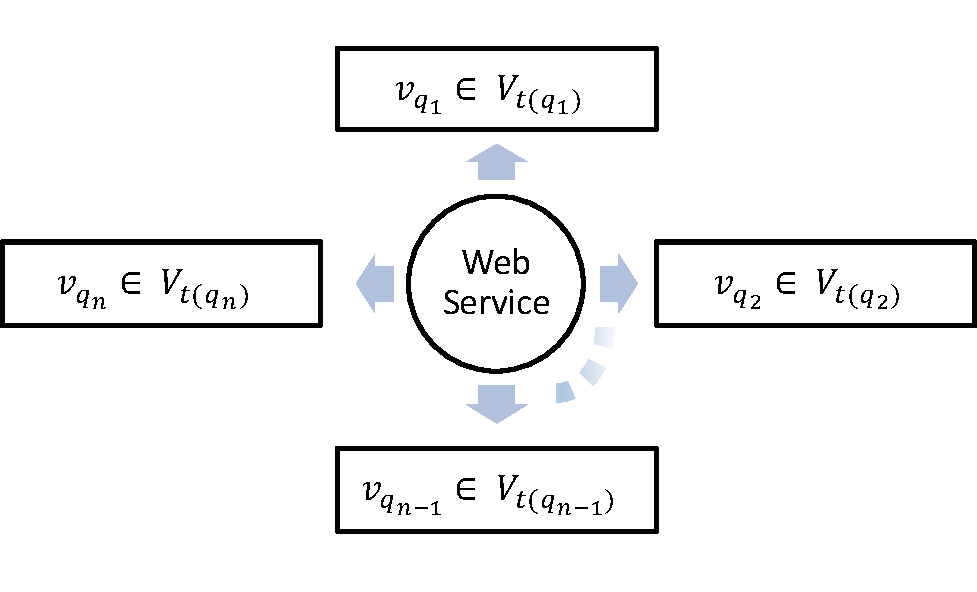
\includegraphics[width=8cm]{ws.pdf}
}}
\caption{Property-Based Web Service Formal Model \cite{agarwal2010d5}.}
\label{fig:ws}
\end{figure}

\subsection{Functional Properties of Web services}\label{functional}

\textbf{A Functionality Model}. This mode is represeted as a Labelled Transition System (LTS): $L = (S,T,\rightarrow)$ comprises a set $S$ of states, a set $T$ of transition labels and a labeled transition relation $\rightarrow \subseteq S \times T \times S$. This transition system is established to present the actual behaviour of web services, which consists of a series of states. See Fig. \ref{fig:lts}.

\begin{figure}
\centerline{
\fbox{
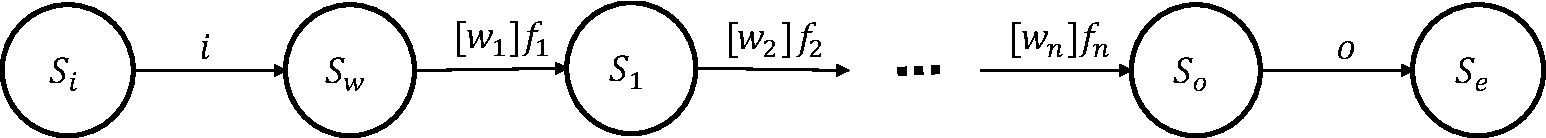
\includegraphics[width=14cm]{LTS.pdf}
}}
\caption{ The functionality of a Web Service \cite{agarwal2010d5}.}
\label{fig:lts}
\end{figure}

\begin{itemize}
\item $S_i$ start state includes knowledge available to web service before the web service is invoked by inputs; 
\item $S_w$ state includes the inputs additional to the knowledge in 1; 
\item A series of state $S_1$ to $S_n$ proceed with corresponding actions $f_n$ that only occurred if each related condition $[w_i]$ is approved to be true. 
\item $S_o$ state contains all the outputs and all the changes performed in the knowledge base. 
\item $S_e$ is the end state, which is equivalent to $S_o$, since the knowledge base is not changed.
\end{itemize}

\textbf{An Abstract Functionality Model}. The first functionality model presented above is not completely demonstrated for the internal actions, as the services provider does not want reveal all the internal functions, and it is not feasible to list a global set of property name. Therefore, an abstract functionality of a web service is modelled by eliminating all the intermediate properties. In the abstract model of a web service, the functional properties of the web service could be identified as inputs $i$, pre-state $S_i$, outputs $o$ and post-state $S_o$. These four properties are mapped to a set of input $I$, preconditions $\phi$, a set of outputs $O$ and postcondition $\varphi$ respectively in third updated functionality model demonstrated below.

\textbf{A Updated functionality Model}. In the updated model, a set of inputs $I$ is required by a service and a set of output $O$ is returend after the successful execution. Apart from that, the precondition $\phi$ must be hold in the knowledge base before service is invoked by passing the input $I$. To enable the interoperability of the functional properties, ontology reasoner is employed to reason about the properties of web services. To distinguish the changes between before and after service execution, these changes are modeled as property instances. For example, inputs and outputs assigned as variable names and further referenced in preconditions and postconditions, which can be distinguished as different instances from the knowledge base. In particular, preconditions is assigned to the description of requirements of inputs using logic formula. Herein the description of the formula considers the following cases that are demonstrated using Planning Domain Description Language (PDDL \cite{fox2003pddl2}):
\begin{itemize}
\item Conditions on the type of inputs, e.g., the payment of an online shopping website is made by Visa or Cash: $\phi:(Format(payment)=Visa \cup Format(payment)=Cash)$.
\item Relationships among inputs, e.g.,  authoried users are required for an online shopping: $\phi:(Authoried ? Useraccount)$.
\item Conditions on the value of inputs, e.g., saving account balance has more than 100 dollars: $\phi: (\geq (amounts, saving account), 100)$
\end{itemize}
These preconditions must be hold in the state consistently while inputs are being passed to services. Similarly, the postcondition is restricted to the description of constraints on returned outputs, relationships between inputs and outputs, and changes caused by the service in the knowledge bases.

\subsection{Nonfunctional Properties of Web services}\label{nonfunctional}
Apart from the functional properties of web services discussed above, the non-functional properties of web services play an important part in composing services. For example, customers prefer lowest execution cost with highest response time and reliability. According to \cite{zeng2003quality}, four most often considered QoS parameters are as follows:
\begin{itemize}
\item \textit{Response time} ($T$) measures the expected delay in seconds between the moment when a request is sent and the moment when the results are received.
\item \textit{Cost} ($C$) is the amount of money that a service requester has to pay for executing the web service
\item \textit{Reliability} ($R$) is the probability that a request is correctly responded within the maximum expected time frame.
\item \textit{Availability} ($A$) is the probability that a web service is accessible.
\end{itemize}

\subsection{Web Service Discovery}\label{servicediscovery}
To generate service compositions, web service must provide mechanisms for discovery required services. Therefore, service discovery must be one fundamental technique to be considered in all service composition approaches. \cite{agarwal2009d5} discussed three mechanisms of semantic web service discovery: classification-based approach, functionality-based approach and hybrid approach. Those service discovery techniques are futher demonstrated below.

The first service discovery technique makes use of the classes provided by service semantic annotation in WSMO-Lite language. Therefore, service requesters can use class names to express a goal offering a straightforward discovery from a set of classes. However, classes without clear meaning definition could lead to the issue of incomprehensibility of web service discovery. For example, serveral classes may declared in either different terms for the describing the same content or same terms for describing different content.

The second service discovery technique  does not take classes into account, but consider functional properties of web service to include pre-conditions and post-conditions. In particular, a desired functionality description is defined. A discovery algorithm must be developed to handle a matching for different input, output, precondition and postcondition with associated concepts and relations in the provided domain knowledge base. The key idea of the matchmaking is to check whether services accept all the desired inputs provided bu users and whether the desired outputs is delivered by services. In addition, the matchmaking algorithm also checks for the satisfiability of implications that actual precondition and actual postcondition must imply the desired precondition and desired postcondition respectively. The strength of the second is that it potentially meet the demands of all the comprehensible discovery, while the weakness is a lack of efficiency and scalability. 

The third service discovery technique is based on a hybridisation of classification and functionality-based discovery. Classification hierarchy is proposed to achieve automatic semantic reasoning in hierarchical functionality. For example, a functionality class is associated with super classes and sub classes for more general functionality class and more specific functionality class respectively. Howvever, to make a consistency of classification hierarchy, the inputs, outputs, precondition and postcondition of a functionality class must satisfy the conditions that contains all the inputs, outputs, precondition and postcondition of all the classes it is subsumed by. The advantage of this approach is to achieve better performance combining strengths of the previous two pure classifications based and functionality based approaches. While the classification hierarchy needs to be kept consistent when a new web service is published or updated.​

The first and third approach is considered either less effective or demands to build up a consistent ontology for classes and their functional attributes. That is not the focuse of our research.  \emph{In the proposal, we use the second service discovery technique for meeting the comprehensible discovery. That is, different types of ontology reasoning are utilised to approach the matchmaking as a fundamental part of service composition algorithm.}



\section{Web Service Composition}\label{overview}

Since one atomic web service could not satisfy or fully satisfy users' complex requirements, web service composition is approached by composing web services together with more sophisticated functionalities to meet the demand. Due to fully human intervention in manual service composition, so it is very time-consuming and less productive. Therefore, many approaches have been developed to achieve semi-automated or fully automated service composition. The semi-automated service composition is inspired by the business process that required prior knowledge to build up the abstract workflow. This workflow can be decomposed into several functional services slots for proper services being fitted. These steps are further discussed in Subsection \ref{lifecycle}. On the other hand, when we are composing services, both semi-automated and fully automated web service composition holds the challenge in the interoperability of services discussed previously. In particular, several problems are simultaneously taken into account. That is I/O matchmaking (i.e., the mechanisms of services for ensuring the interoperability ), discovery relevant services to the optimising the quality of service composition, e.g., overall QoS. Consequently, the following concerns are required to consider in generating composition solution. 


\subsection{Web Service Composition Lifecycle}\label{lifecycle}
Typical steps in a workflow-based automated Web service composition solution are shown in Fig. \ref{fig:lifecycle}. The detail of the service lifecycle is discussed as follows:

\begin{figure}
\centerline{
\fbox{
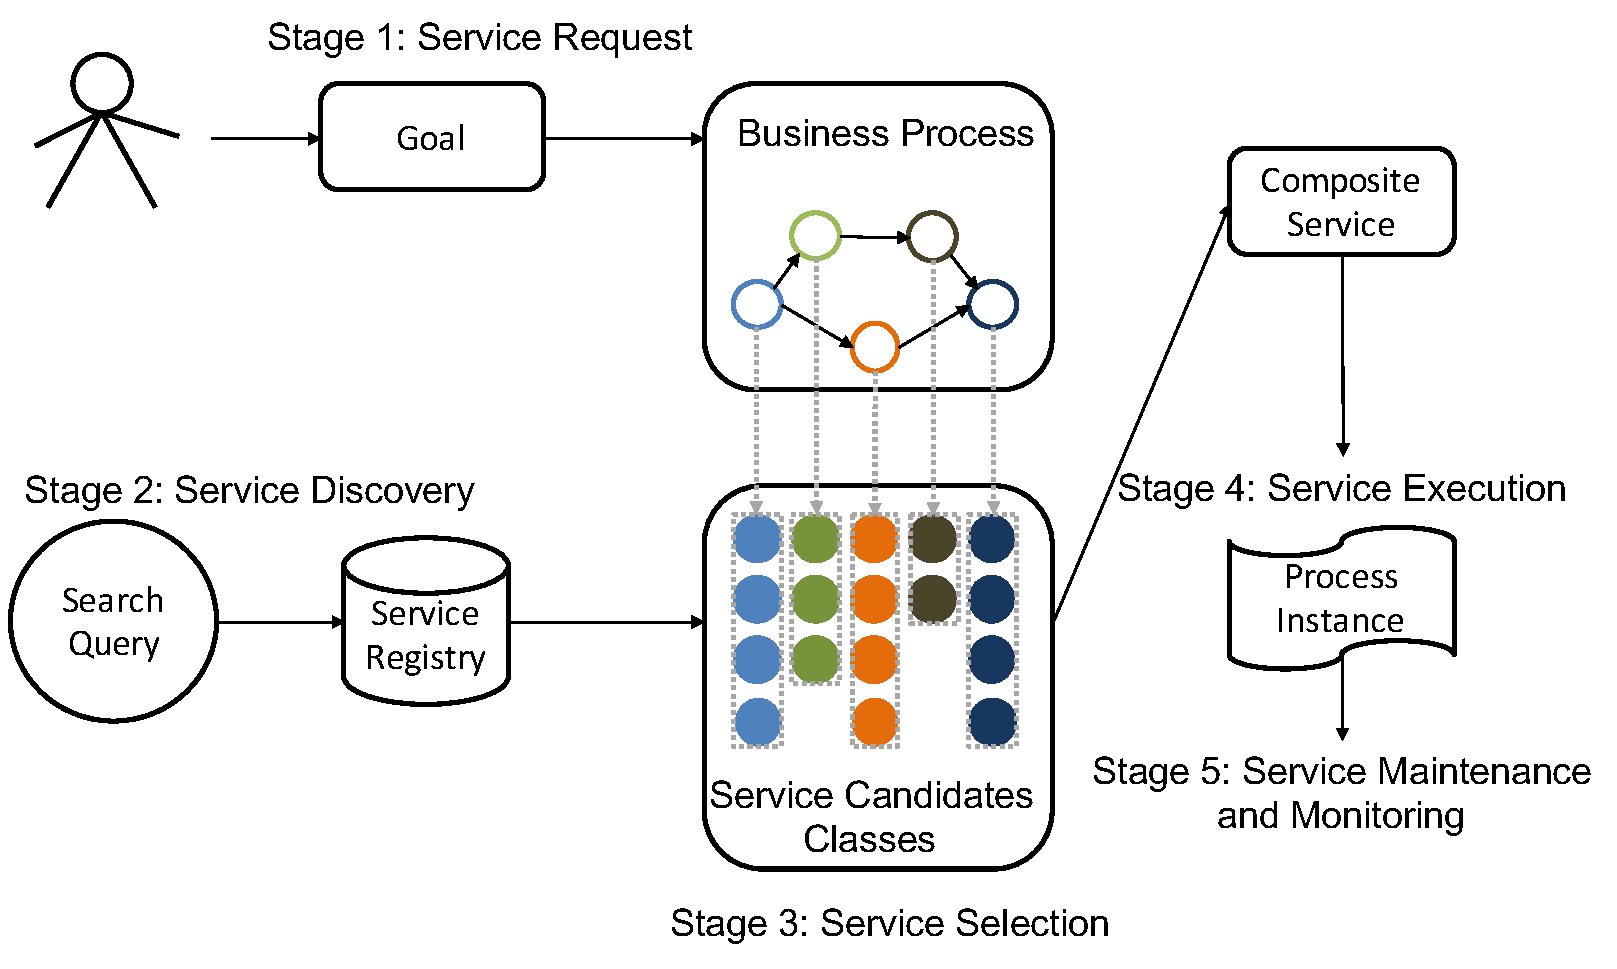
\includegraphics[width=14cm]{compositionLifecycle.pdf}
}}
\caption{ Web service composition lifecycle \cite{moghaddam2014service}.}
\label{fig:lifecycle}
\end{figure}

\begin{enumerate}
 \item \textit{Goal specification:} The first step in service composition is to collect users' requirements for composition goal that comprises of the functional (i.e., correct data flow ) and non-functional side (i.e., QoS). This step is achieved by building up an abstract workflow including a series of tasks with clearly defined functionality. Those tasks could be completed by selecting proper concrete services to reach desired QoS. 
 \item \textit{Service discovery:} Once the goal is clearly specified, concrete web services are to be selected for each task regarding its functional requirement. Often, more than one concrete web service is likely to be found to match the one task. However,  those matched web services are always different in QoS.  Therefore, web services are classified by the functionality of each task, i.e., inputs and outputs.
 \item \textit{Service selection:} At this stage, many techniques have been studied to select web services to best match each task for the satisfying functional requirement of each task and overall business process. Therefore, a plan of service composition is created ahead of execution.

 \item \textit{Service execution:} the process instance is monitored for any changes or services failures during service execution. In this stage, some actions are to be taken for adapting the changes.
\end{enumerate}
The web service lifecycle discussed above is a typical \emph{semi-automated approach}. There is a distinction between semi-automated and fully automated approaches. On the one hand, during the goal specification stage of semi-automated approach, the abstract work is already provided.  On the other hand, an abstract workflow is not provided at the stage of goal specification for \emph{fully automated service composition}. Often, fully automated service composition rely on some algorithms (e.g., Graphplan algorithm \cite{blum1997fast}) to achieve service composition, during which service workflow is gradually built up along with the service discovery and service selection at the same time. In this proposal, I concentrate on developing methods for fully automated service composition since it has been shown the flexibility. Also, herein service discovery and service selection are considered as interrelated tasks that are interleaved with the composition algorithm.

\subsection{Functional Properties of Web Service Composition}
Substantial work \cite{bansal2016generalized,lecue2009optimizing, lecue2007making, lecue2006formal, rao2005semantic} on semantic web service composition utilises Description logic (DL) reasoning between input and output parameters of web services for matchmaking. OWL and OWL-S are the most common semantic specifications used currently \cite{petrie2016web}, and they enable automatic selection, composition, and interoperation of Web services to implement complicated composition tasks \cite{martin2004owl}. However, some matchmaking types (discussed below) may penalise the matchmaking quality and are less prefered by users. Therefore, exploring a effective mechanism for measuring the quality of semantic matchmaking in serivce composition is a very demanding research area.

Given two concepts $a, b$ in ontology $\mathcal{O}$, four commonly used \emph{Matchmaking types} are often used to describe the level of a match between outputs and inputs \cite{paolucci2002semantic}: 
\begin{itemize}
\item the \emph{matchmaking} returns $exact$ if $a$ and $b$ are equivalent ($a \equiv b$), 
\item the \emph{matchmaking} returns $plugin$ if $a$ is a sub-concept of $b$ ($a \sqsubseteq b$),
\item the \emph{matchmaking} returns $subsume$ if $a$ is a super-concept of $b$ ($a \sqsupseteq b$), 
\item the \emph{matchmaking} returns $fail$ if none of previous matchmaking types is returned. 
\end{itemize}

Often, the similarity of two instances of two knowledge representations encoded in the same ontology is also utilised to measure the quality of matchmaking regarding the four matchmaking types discussed above. The work \cite{lecue2007making} additionally consider $interaction$ matchmaking type ($a \sqcap b$), i.e., if the intersection of $a$ and $b$ is satisfiable. In their work, a causal link link \begin{math} sl_{i,j} \stackrel{.}{=} \langle S_i, Sim_{T}(Out\_s_i,In\_s_j),S_j  \rangle \end{math} is created between two functional property instances for a input and a output. In particular, both $exact$ match and $plugin$ match are presented as robust causal links, while both $subsume$ match and $intersection$ match are presented as valid casual links. However, valid casual links are not specific enough to be utilised as the input of another web service. Thus the output requires Extra Description Equation \ref{equation2} to enable proper service composition. As a result, Subsume and Intersection matching type is transferred to be Exact and PlugIn respectively to formulate a robust link. 

\begin{equation}
In\_s_x \setminus Out\_s_y \stackrel{.}{=} \underset {\preceq d}{min} \{ B|B\sqcap  Out\_s_y \equiv In\_s_x  \} , since \  Out\_s_y \sqsupseteq In\_s_x
 \label{equation2}
\end{equation}



\emph{In this paper we are only interested in robust compositions where only $exact$ and $plugin$ matches are considered, see \cite{lecue2009optimizing}. As argued in \cite{lecue2009optimizing} $plugin$ matches are less preferable than $exact$ matches due to the overheads associated with data processing. We suggest to consider the semantic similarity of concepts when comparing different $plugin$ matches.}

\emph{Robust causal link} \cite{lecue2008optimizing} is a link between two matched services $S$ and $S'$, noted as $S \rightarrow S'$, if an output $a$ ($a \in {O_S}$) of $S$ serves as the input $b$ ($b \in {O_{S'}}$) of $S'$ satisfying either $a \equiv b$ or $a \sqsubseteq b$.  For concepts $a, b$ in $\mathcal{O}$ the \emph{semantic similarity} $sim(a, b)$ is calculated based on the edge counting method in a taxonomy like WorldNet or Ontology \cite{shet2012new}. This method has the advantages of simple calculation and good performance \cite{shet2012new}. Therefore, the \emph{matchmaking type} and \emph{semantic similarity} of a robust causal link can be defined as follow:

\begin{align}
\label{eq_link}
type_{link} = 
\begin{cases}
	1 & \text{ if $a\equiv b$ ($exact$ match)}\\
	p & \text{ if $a \sqsubseteq b$ ($plugin$ match)}
\end{cases}
,&&
sim_{link} = sim(a,b) = \frac{2N_c}{N_{a}+N_{b}}
\end{align}

\noindent with a suitable parameter $p, 0<p< 1$, and with $N_a$, $N_b$ and $N_c$, which measure the distances from concept $a$, concept $b$, and the closest common ancestor $c$ of $a$ and $b$ to the top concept of the ontology $\mathcal{O}$, respectively. However, if more than one pair of matched output and input exist from service $S$ to service $S'$, $type_e$ and $sim_e$ will take on their average values.

The \emph{semantic matchmaking quality} of the service composition can be obtained by aggregating over all robust causal links as follow:
\begin{align}
MT {=} \prod_{j=1}^{m} type_ {link_{j}}
,&&
SIM {=} \frac{1}{m}\sum_{j=1}^m sim_ {link_{j}}  
\end{align}


\subsection{Nonfunctional Properties of Web Service Composition}
The aggregation value of QoS attributes for web services composition varies with respect to different constructs, which reflects how services associated with each other in a service composition \cite{zeng2003quality}.

We use formal expressions as in \cite{ma2012formal} to represent service compositions. We use the constructors $\bullet$, $\parallel$, $+$ and $\ast$ to denote sequential composition, parallel composition, choice, and iteration, respectively. The set of \emph{composite service expressions} is the smallest collection $\mathcal{SC}$ that contains all atomic services and that is closed under sequential composition, parallel composition, choice, and iteration. That is, whenever $\cse_0,\cse_1,\ldots,\cse_d$ are in $\mathcal{SC}$ then $\bullet(\cse_1,\ldots,\cse_d)$, $\parallel(\cse_1,\ldots,\cse_d)$, $+(\cse_1,\ldots,\cse_d)$, and $\ast \cse_0$ are in $\mathcal{SC}$, too. Let $\cse$ be a composite service expression. If $\cse$ denotes an atomic service $S$ then its QoS is given by $QoS_S$.  Otherwise the QoS for $\cse$ can be obtained inductively as summarized in Table~\ref{tbl:QoS_Aggre}. Herein, $p_1,\ldots,p_d$ with $\sum\limits^d_{k=1}p_k=1$ denote the probabilities of the different options of the choice $+$, while $\ell$ denotes the average number of iterations.

\begin{table}[htb]
\centering
\caption{QoS calculation for a composite service expression $\cse$}
\begin{tabular}{l|l|l|l|l}
\hline
 $\cse=$       &$r_\cse=$                              &$a_\cse=$                              &$c_\cse=$                            &$t_\cse=$ \\ \hline
 $\bullet(\cse_1,\ldots,\cse_d)$      &$\prod\limits^d_{k=1}r_{\cse_k}$    &$\prod\limits^d_{k=1}a_{\cse_k}$    &$\sum\limits^d_{k=1}c_{\cse_k}$   &$\sum\limits^d_{k=1}t_{\cse_k}$  \\ \hline
 $\parallel(\cse_1,\ldots,\cse_d)$  &$\prod\limits^d_{k=1}r_{\cse_k}$    &$\prod\limits^d_{k=1}a_{\cse_k}$    &$\sum\limits^d_{k=1}c_{\cse_k}$   &$MAX \{ t_{\cse_k} | k \in \{ 1,...,d \} \}$\\ \hline
 $+(\cse_1,\ldots,\cse_d)$     &$\prod\limits^d_{k=1}p_k\cdot r_{\cse_k}$    &$\prod\limits^d_{k=1}p_k\cdot a_{\cse_k}$    &$\sum\limits^d_{k=1}p_k\cdot c_{\cse_k}$   &$\sum\limits^d_{k=1}p_k\cdot t_{\cse_k}$  \\ \hline
 $\ast \cse_0$         &${r_{\cse_0}}^\ell$  &${a_{\cse_0}}^\ell$  &$\ell\cdot c_{\cse_0}$ &$\ell\cdot t_{\cse_0}$ \\ \hline
\end{tabular}
\label{tbl:QoS_Aggre}
\end{table}




%Besides identifying the atomic Web services most suitable to fulfilling key composition tasks, the selection process often takes additional user constraints into account. A survey of the literature in the area shows that two types of contraints are commonly taken into account. The first group comprises the creation of service compositions that are optimised according to the Quality of Service (QoS) constraints on its constituent atomic services, where QoS attributes may be thought of as features that indicate the quality of a given Web service, such as the time it requires to return a response and its financial cost of execution \cite{da2014graph}. The majority of works in this area use maximising and minimising functions for the different QoS attributes, meaning that they attempt to obtain solutions with the best possible qualities without any thresholds \cite{wang2013improved,parejo2008qos,yoo2008web,garcia2008qos,zhang2010qos,wang2012survey,moghaddam2014service,kattepur2013qos,DBLP:journals/soca/LiZDSGL13}. However, there also exist approaches focused on what may be referred to as a Service Level Agreement (SLA)-aware optimisation, which is solutions must meet certain predetermined QoS thresholds in order to be considered valid (e.g. the financial cost of each service used in a composition must not exceed 50 dollars) \cite{yoo2008web,yin2014hybrid,chen2014partial,berg2013revenue}.

%The second group comprises the creation of service compositions that have multiple execution branches, indicating user preferences at runtime \cite{wang2014automated,boustil2010web,karakoc2009composing,marconi2006specifying,bertoli2009control}. For example, the output of a service \textit{A} determines which service to execute next; if the output is greater than a certain threshold, then service \textit{B} should be executed; otherwise, service \textit{C} should be executed instead. These preferences are expressed logically as conditions, and affect the workflow used to establish the connections between services rather than the individual services themselves. These two types of user constraints are discussed in more detail in subsequent Sections in this chapter.

%\subsection{Web Service Composition in Practice}

%The research material published on Web service composition is highly theoretical and frequently employs layers of abstractions and simplifications intended to make the problem at hand manageable. However, it is also important to investigate how these ideas fit into practice, which is the objective of this Subsection. As mentioned earlier, while significant amounts of work are being performed in the field of automated Web service composition, these approaches ultimately remain on the theoretical level due to difficulties that have not yet been fully addressed. On the one hand, a study \cite{lu2007web} has shown that the composition of services is fraught with issues. A central problem is that there are discrepancies between the concepts used by different services: the schemas used differ from each other, even if the services handle exactly the same domain. Another problem is the existence of services that produce too much data, low-quality data, or that incur too much latency. These characteristics may slow down the execution of the composition and even require human intervention, defeating automation efforts.

%On the other hand, an automated framework for Web service compositions which can be applied to real services has already been proposed \cite{marconi2007automatedweb}.
%The functionality of this framework was demonstrated by creating a composition that uses the Amazon Virtual Cart service, the Amazon
%Book Search service and a bank's Point of Sale Web service. The authors of the framework point out that it is very challenging to find service documentation that is comprehensive enough, and that functionality details had to be identified from natural language explanations intended
%for developers who are working manually. Additionally, the specification of control flow requirements must be performed manually using a logic programming language. Despite these difficulties, the evaluation of this framework shows that a composition can be found within seconds when using it as opposed to an estimated 20 hours of manual development, showing that research on Web service composition provides some immediate benefits.

%These two works provide opposing views on the viability of automated Web service composition, however a more recent approach \cite{mobedpour2013user} presents the interesting middle ground of user-centered design. This systems combines manual and automated techniques, providing a browsing tool that allows users to explore the repository and gain some understanding of the offered QoS value ranges of services before having to write any QoS requirements, as users may often be unaware of what a reasonable QoS value would be for a given dataset. Users are also supported through the selection process by utilising a UI that diminishes their cognitive overload, and helps them express their requirements using a standardised language. In addition to these tools, this approach also proposes a clustering algorithm that groups service candidates according to their range of QoS values, with the objective of providing selection options when users have fuzzy (i.e. soft) requirements. The strength of this approach is that it does not undervalue human intervention in the composition process, instead providing tools that empower system users. As Web service composition always requires some degree of user involvement, at the very least when setting composition requirements, this type of approach may prove to become an increasingly popular composition solution.

%\section{Single-Objective QoS-Aware Composition Approaches}\label{SingleObjective}

%This section discusses composition approaches that optimise solutions according to their overall QoS. These approaches can be divided into biologically inspired methods, which use Evolutionary Computation to reach their goal, ang general optimisation approaches that do not turn to evolutionary techniques. These two groups are quite distinct, but they have the commonality of using an objective function as the guide with which to measure the quality of the candidate solutions.

%\subsection{Biologically-Inspired Approaches}

%Biologically-inspired Web service composition approaches rely on evolutionary computation algorithms, which implement their search strategies by drawing inspiration from nature, namely the behaviour of social animals such as bees, fish, and ants. An important distinction between these different bio-inspired approaches is in their representations of the composition problem. These varying representations are discussed throughout this Subsection, and visually summarised in figure \ref{fig:representations}. \textbf{Genetic Algorithms (GA)} are a popular choice for tackling combinatorial optimisation problems, and thus have been widely applied to the problem of Web service composition \cite{wang2012survey}. The encoding scheme for a composition is commonly done as a vector of integers, where each integer corresponds to a candidate Web service, even though some authors have attempted to use matrix representations that also include semantic information about services. A population of candidates is evolved for several generations using generic operators, typically crossover and mutation: in crossover, equivalent sections of the vectors in two distinct candidates are swapped; in mutation, a section of one candidate's crossover is modified at random in order to introduce some genetic diversity. An observed problem with the GA technique is that it tends to prematurely converge to solutions, thus preventing the exploration of further possibilities. \textbf{Particle Swarm Optimisation (PSO)} bears similarities with GA, also relying a on vector representation for candidates. However, instead of employing genetic operators to carry out the search process, PSO uses the concept of position updates to move candidate particles across the search space. As PSO may also present the problem of not fully optimising solutions (i.e. converging prematurely), hybrid approaches have been attempted to improve its efficiency and optimisation power \cite{wang2012survey}. A key limitation of both GA and PSO is in the underlying vector representation used by candidates, since it makes it very challenging to encode workflow information and thus perform any type of fully automated Web service composition.

%\begin{figure}
%\centerline{
%\fbox{
%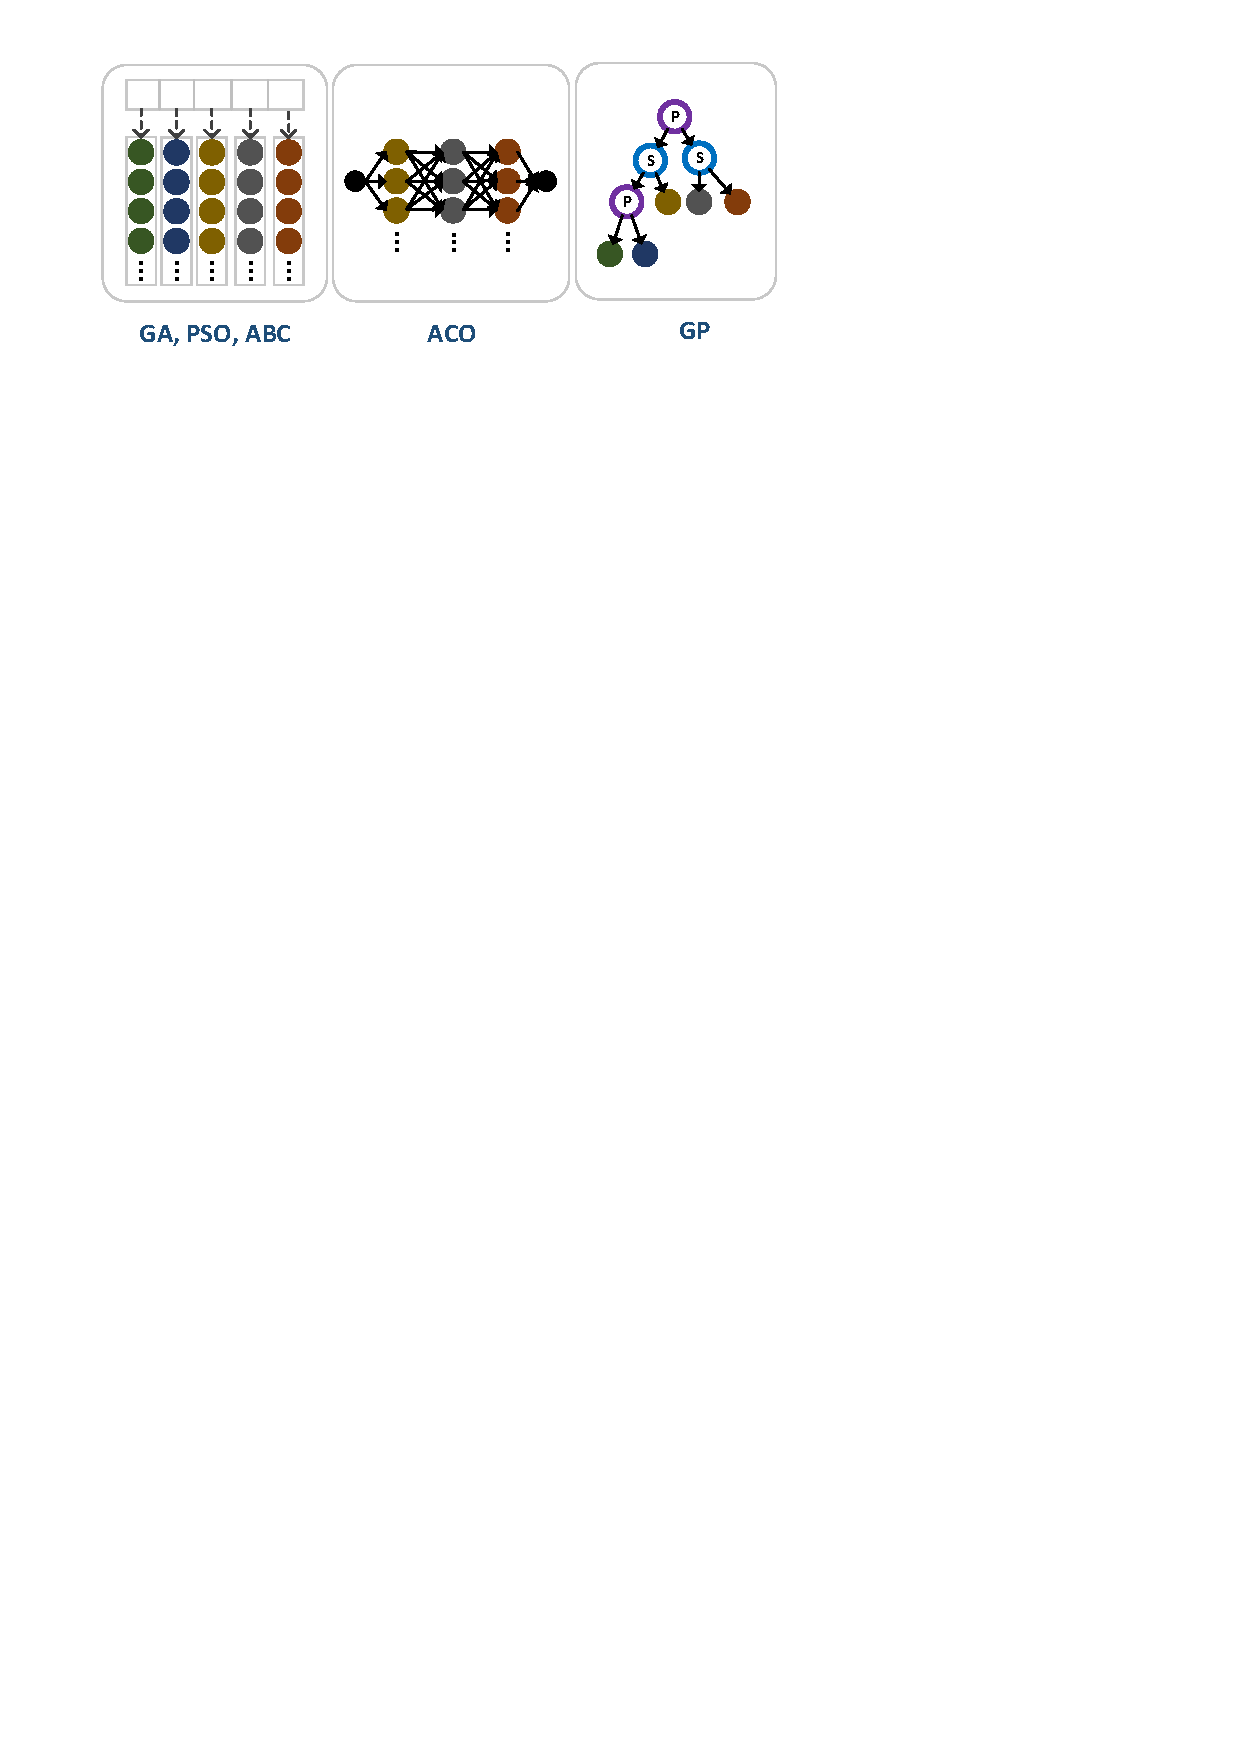
\includegraphics[width=14cm]{representations.pdf}
%}}
%\caption{The different problem representations employed by biologically-inspired Web service composition approaches.}
%\label{fig:representations}
%\end{figure}

%\textbf{Ant Colony Optimisation (ACO)} has also been proposed as a solution to QoS-aware Web service composition \cite{zhang2010qos}. ACO is particularly suitable to a directed acyclic graph (DAG) representation, in other words, the workflow composition representation commonly used in the field. In ACO, the Web service workflow is built to be traversed by a group of ants (agents). At each fork in the graph, the ants choose which path to follow based on probabilities that take into account the strength of the pheromones left by other ants, and also a heuristic function for that particular graph. The pheromones left by the ants are updated after all ants have toured through the graph once, with paths of higher fitness resulting in a larger pheromone increment for the edges of those paths. Meanwhile, the pheromone level of all edges gradually decreases (i.e. evaporates) after each tour of the ants. The graph representation in this technique follows the abstract workflow idea, with a pool of concrete Web services associated to each abstract Web service. Each pool of candidates is a layer that is fully connected to the layers of any following abstract services, so that an optimal path can be chosen from the edges laid out. For each concrete Web service, the heuristic factor is calculated based on its QoS values, and the fitness function also measures QoS attributes. As with GA and PSO, this representation also amounts to the idea of semi-automated Web service composition, even though in this case the encoding of workflow information leading to a fully-automated approach would seem to be trivial.

%The works in \cite{zhang2010qos} and \cite{wang2013improved} apply the \textbf{Artificial Bee Colony (ABC)} algorithm to Web service composition. The ABC algorithm simulates the behaviour of bees search for food sources. The position of food corresponds to candidate solutions in the search space, encoded as a service vector, and there are three types of bees dedicated to searching: \textit{Employed bees} exploit the neighbourhood of a single food source already found; \textit{Onlooker bees} exploit the neighbourhood of different food sources depending on the dance behaviour displayed by employed bees; \textit{Scout bees} are the bees sent to random food sources after the neighbourhood they were previously exploiting does not present any food sources that are better than the original. The roles of the bees change according to the colony's needs, which is a feature unique to this algorithm. One of the issues with this approach, as pointed out by the authors, is the search space it explores. The problem with the typical search space for Web service composition is that it is organised based on the proximity of the components included into the composition. For example, given two adjacent solutions $a$ and $b$ in the search space, $a$ will only have one service that is different from all the services included in $b$. Despite being neighbours, however, the fitness values of $a$ and $b$ may be radically different, and as the optimisation occurs according to a fitness function, this means that the search space is not entirely continuous. These works modify the traditional ABC algorithm to take this problem into account, filtering the neighbourhood of each solution during the search and excluding radically different neighbours from consideration.

%\textbf{Genetic Programming (GP)} is, from this project's perspective, possibly the most interesting technique for the problem of Web service composition. That is because GP, unlike the previously discussed techniques, is capable of supporting fully automated Web service composition. In GP approaches \cite{aversano2006genetic,rodriguez2010composition}, workflow constructs are typically represented as the GP tree's non-terminal tree nodes while atomic Web service are represented as the terminal nodes. In this context, workflow constructs represent the output-input connections between two services. For example, if two services are sequentially connected, so that output of service \textit{A} is used as the input of service \textit{B}, this would be represented by a sequence workflow construct having \textit{A} as the left child and \textit{B} as the right one. The initial population may be created randomly, in which case the initial compositions represented in that generation are very unlikely to be executable due to their mismatched inputs and outputs, or it may be created using an algorithm that restricts the tree structure configurations allowed in the tree to feasible solutions only. A fitness function is employed for the QoS optimisation of candidates, and the genetic operators employed for this evolutionary process are crossover, where two subtrees from two individuals are randomly selected and swapped, and mutation, where a subtree for an individual is replaced with a randomly generated substitute. One of the difficulties of tackling the problem of Web service composition using GP is that it does not intrinsically support the use of constraints \cite{craenen2001handle}, meaning that even if all candidates in a population meet the feasibility constraints, there is no guarantee that subsequent generations will maintain conformance to them. The approaches discussed above handle this problem in one of two ways: by \textit{indirect constraint handling}, where feasibility constraints are incorporated into the fitness function so that the optimal function value reflects the satisfaction of all constraints, or by \textit{direct constraint handling}, where the basic GP algorithm is adapted at the initialisation and genetic operation stages to ensure that the feasibility constraints are met. Indeed, the tree representation of an underlying workflow composition may pose difficulties whenever constraint verification is necessary.

%\subsubsection{Graph Variations of GP}

%Genetic programming using candidates constructed as graphs (instead of trees) would be ideal for the problem of Web service composition, since dependencies between services could be intuitively encoded. Even though variations of GP with graph candidates do exist, they have not been employed in this domain, therefore the focus of this section is on the techniques and not on the composition problem. Galvan-Lopez \cite{galvan2008efficient} proposes a general-purpose EC technique that is modification of the usual GP tree reprentation, allowing the creation of graphs. The key extension proposed here is the addition of pointer functions to certain non-terminal nodes, meaning that they can have connections to nodes in independent subtrees. Program inputs are provided as terminal nodes (similarly to the output-as-root representation discussed earlier), but instead of having a single output location at the root node, they may have other output locations as well, inserted as necessary amongst the non-terminal nodes of the tree. Since the overall tree structure is maintained, it becomes possible to perform the crossover and mutation operations similarly to their implementation in the case of a simple tree. The main difference is that any pointers present in the original tree may not be modified when these operations are applied. In order to ensure that the number of outputs in a tree remains correct throughout these genetic operations, each node in a tree is classified beforehand to establish which ones may be selected for the crossover operation. This representation makes it easier to evolve graphs, however it does not support strongly-typed GP, which is of interest to our research. In addition, each tree is still required to have a single root, meaning that there are connections between the different output nodes. In our problem domain, this is a hindrance because the output nodes must be completely independent from each other.

%Miller and Thomson \cite{miller2000cartesian} present Cartesian Genetic Programming (CGP), a popular technique for evolving graph structures. The simplicity of SGP lies in the fact that it can represent the genotype of candidates as a string of fixed length, meaning that crossover and mutation operations are trivial to implement provided that they obey some simple constraints. The core idea of CGP is to create a two-dimensional array of programmable nodes of a predefined size. Each node has a predefined number of outputs, and the overall array has a predefined number of inputs and outputs. Then, as this structure is evolved, the functions inside of each node can be reprogrammed, and so can the inputs those nodes require. From that point onward, the structure can be optimised according to the algorithm's fitness function. One important observation is that CGP may have unexpressed genes, meaning that not all the nodes in the two-dimensional array are necessarily components of the final answer. One limitation of this approach is that CGP does not easily handle strongly-typed GP, thus restricting the range of problems it can be applied to. Another problem is that it requires predefined numbers of nodes and node inputs/outputs, making it difficult to represent compositions with varying numbers of services and service inputs/outputs.

%Mabu, Hirasawa and Hu \cite{mabu2007graph} introduce a technique for the evolution of graph-based candidates, called Genetic Network Programming (GNP). GNP has a fixed number of nodes within its structure, categorised either as processing nodes (responsible for processing data) or as judgment nodes (perform conditional branching decisions), and works by evolving the connections between these fixed nodes. Connections are represented in a linear gene structure, and the number of outgoing connections from a node is dependent on the type of that node: processing nodes have a single outgoing connection, while judging nodes have more than one (depending on the number of branches desired). Because of the linear representation of connections between nodes, the genetic operators employed for the evolutionary process are quite simple. The mutation operator randomly chooses the destination of a node's outgoing connection; the crossover operator swaps two nodes with the same label from two different solutions, taking their outgoing edges with them. Li, Yang and Hirasawa \cite{li2014evolving} extend the basic GNP idea by using the Artificial Bee Colony (ABC) approach to evolve candidates. While these approaches present the advantage of simple genetic operations, the number of nodes and outgoing edges per node must be fixed throughout the evolutionary process, meaning that it suffers from the same limitations discussed above.

%Poli \cite{poli1996parallel} presents an EC algorithm where solutions are represented directly as graphs. This graph is mapped to a grid, where each row represents a layer of the graph, and columns can be used freely to accommodate the nodes in a layer. By using this representation, it is possible to perform relatively simple mutation and crossover operations to a graph without compromising its syntactic correctness. For the crossover operation, a crossover point (node) is selected in each candidate, and all the ancestors of that node are identified. These two subgraphs of ancestors are then swapped, a process that may overwrite nodes from the other graph but that maintains any original edges. Whenever this swap causes parts of the subgraphs to be placed outside of the grid, these nodes are "wrapped around" their respective rows, meaning that they are moved to the other extreme of the row. For the mutation operator, an existing subgraph is selected and replaced with a newly created one, using the same general mechanism as the crossover. Once again, while this approach makes the implementation of genetic operations simple, it does not allow for correctness constraints (i.e. input-ouput connections) to be maintained. Additionally, this representation assumes that the duplication of nodes is acceptable, which may pose some problems in the domain of Web service composition.

%Kantschik and Banzhaf \cite{kantschik2002linear} propose linear-graph GP, a structure that allows programs with multiple execution paths to be optmimised using evolutionary computing. This approach is an extension of the simple linear program representation where each element of a vector contains one program instruction. In this representation, a program graph contains several nodes, and each of these nodes contains a portion of a linear program that may be executed according to preceding branching conditions. Within each of these nodes, there exists also a branching node that is responsible for determining which outgoing edge to follow (i.e. which execution path to choose after executing the current node). The branching functions contained in each of these nodes may read the values of variables manipulated in the linear program portion that is located in the same graph node. The mutation operator in this approach may alter an individual entry within a linear program vector, the branching function within a branching node, or the number of outgoing edges of a given graph node; the crossover operator may exchange individual entries within linear vectors of two candidates, or exchange a group of contiguous graph nodes between two graphs. Despite allowing branching constructs, this approach is not useful to our research because non-sequential relationships between different Web services cannot be encoded into linear representations.

%The works in \cite{globus1999automatic,brown2004graph,nicolaou2009novo} present a graph-based genetic algorithm that is used to evolve representations of molecules. Atoms are represented as nodes, and their bonds as edges. Two types of genetic operations are supported: mutation, which can be the appending or removing of a node and its connecting bonds,
%and crossover, where edges are removed from each candidate until each graph is divided into two disconnected subgraphs that are then reconnected to create new child candidates. The reason why these genetic operators can be used without compromising the strucuture of the molecule is that the only restriction when creating a new connection is the valence of a given atom (i.e. the number of bonds it can make), but bonds do not need to be directed edges and cyclic structures are allowed. In the Web service composition domain, however, the need for additional restrictions means that these genetic operators are no longer suitable.

%\subsection{Other Optimised Composition Approaches}

%Other methods exist for producing optimised Web service composition results in addition to biologically inspired approaches, and a subset of them is presented in this section. \textbf{Tabu search} \cite{glover1989tabu} is a combinatorial optimisation strategy for identifying an optimised solution amongst a group of candidates, typically in problems where exhaustive search is prohibitively expensive. In Tabu search, an objective function (either linear or nonlinear) is used to measure the goodness of solutions, encouraging solutions with the least penalty (i.e. optimal solutions). Then, a range of moves that lead from one candidate solution to another is defined. For a particular candidate solution,
%there is a set of moves that can be applied to it, and this is known as the neighbourhood function. One of the biggest advantages of Tabu search is that, unlike the
%hill climbing technique, it can avoid being stuck at local optima when searching. The technique keeps track of a set of tabu moves, which are moves that violate a given
%collection of tabu conditions. The objective of having a tabu set is to prevent the search from reaching solutions whose best next move has already been visited (i.e. prevent cyclic search moves). Due to its relative simplicity and its flexibility of implementation, tabu search has a wide range of practical applications for combinatorial
%optimisation problems. For example, a technique that combines Tabu search and a hybrid Genetic Algorithm (GA) implementation has been proposed recently \cite{parejo2008qos}. For the Tabu search component of the technique, a move is defined as a change in one of the concrete services used as the solution, and the Tabu set is a fixed-size set of the latest
%\textit{n} solutions visited. For the hybrid GA, the same basic idea of the traditional GA is applied (set candidate sizes, two-point crossover, mutation that randomly chooses another concrete service), however a local improver is also employed. This improvement process randomly explores a percentage of a solution's neighbourhood. A drawback of using Tabu search for Web service composition is that the structure used for the representation of candidates is typically linear \cite{parejo2008qos,bahadori2009optimal}, which restricts the problem model to address semi-automated compositions only.

%\textbf{Integer Linear Programming (ILP)} has also been applied to composing Web services \cite{yoo2008web}. ILP is flexible in the way it represents problems, therefore a fully automated Web service composition approach that also takes non-functional attributes into account when constructing the best solution can be solved using it. An objective function is defined for the achieving the optimal QoS values, and several other functions are used to restrict the functionality of the solutions (i.e. restrict the search space). For linear programming, we first determine the "corners" of the restricted search space (i.e. where two constraint lines meet), and then apply the objective function to each of these solutions. One of these "corner" solutions is the optimal one, provided that all boundary functions are linear, so the best objective function score indicates the final solution. While ILP applied to Web service compositions is guaranteed to find an optimal solution, it has been shown to be very inefficient in comparison to EC-based approach as the complexity of the problem increases \cite{aversano2006genetic}. Another problem with the ILP approach is that it is likely to pose difficulties when used for creating compositions with multiple execution paths, as branching constraints would have to be represented using a linear function.

%\textbf{Structural Equation Modelling (SEM)}, a statistical analysis method for forecasting values according to current measurements, has been used in a service selection strategy that considers the future trends of the QoS values of the candidate services \cite{DBLP:journals/soca/LiZDSGL13} as opposed to relying on static QoS snapshots. By being able to predict the QoS trends of services, it is possible to create a composition that is optimal at execution time. One key advantage of SEM is that it is capable of accommodating changes in the user preferences (weights) associated with each QoS attribute, and can use the errors in QoS measurement histories to create a forecast model. The proposed approach was tested using different composition algorithms (e.g. ILP) enhanced with SEM, with a dataset that simulates the changes of QoS parameters over time. Results show that the prediction model for QoS values is initially quite inaccurate, but the accuracy increases for both algorithms as days go by and a history of values is built. While this method is very effective at predicting QoS values to aid in the optimisation of solutions, it cannot be used alone to compose Web services. Thus, SEM is not considered further in this work.

%Finally, \textbf{Algebraic Expressions (AE)} have been employed to the problem of Web service composition \cite{ferrara2004web, kattepur2013qos}. A formal representation of a Web service composition is used in this approach, relying on algebraic constructs to describe the behaviour of atomic Web services and to constraint the characteristics of a correct composition solution. One of the main advantages of AE is that this technique is expressive enough to emulate the behaviour of Web service composition languages such as BPEL4WS, thus it is possible to design and verify composition solutions entirely through AE. A more flexible composition option, explored in \cite{ferrara2004web}, involves constructing a mapping between algebraic expression and BPEL, to allow for an automated translation between these two representations. The work in \cite{kattepur2013qos} goes further, proposing a composition algorithm that also performs QoS optimisation based on algebraic expressions. Despite promising, the disadvantage of this technique is that it requires the composition task to be described in formal terms that are challenges to system users without the necessary background.

\section{Multi-objective, and Many-objective Composition Approaches}\label{MultiObjective}

%\begin{equation}
%fitness_i = w_1A_i + w_2R_i + w_3(1 - T_i) + w_4(1 - C_i)
%\end{equation}

%\centerline{where $\sum_{i=1}^{4} w_i = 1$}
%\vspace{0.7cm}
%----------------------chen starts---------------------------------------------------
Maximising or minimising a single objective function is a most commonly used way to handle optimising problems in automated web service composition.  That is a Simple Additive Weighting (SAW) \cite{hwang1981lecture} technique, which presents a utility function for all the individual quality criteria as a whole. This technique optimises and ranks each web service composition using a single value for each solution. However,  the limitation of this technique lies in not handing the conflicting quality criteria.  Those conflicting quality criteria are always presented trade-offs. To overcome this limitation, a set of objectives corresponding to different independent quality criteria are optimised independently. Consequently,  a set of promising solutions that present many quality criteria trade-offs are returned.


\subsection{Multi-objective approaches}\label{MultiObjective}

Many multi-objective techniques \cite{liu2005dynamic,zhang2010qos,yu2013efficient,yin2014hybrid,xiang2014qos,chen2014partial} have been investigated to extensively study QoS-aware web service composition problems.  A set of optimised solutions is ranked based on a set of independent objectives, i.e., different QoS attributes. In particular, solutions are compared according to their relationship for domination. Especially, figuring out solutions are clearly dominating the others. For example, given two service composition solutions that are compared based on execution cost $c$ and execution time $t$, solution one, $wsc_1(c=10,t=1)$ and solution two,  $wsc_2(c=13,t=1)$. In our context, $wsc_1$ dominate $wsc_2$ as $wsc_1$ has the same execution time and a lower execution cost. If given $wsc_3(c=10,t=2)$, $wsc_2$ is a \textit{non-dominant} solution in the relation to $wsc_3$ because of its longer execution time and cheaper execution cost. Therefore,  If those non-dominant solutions are globally produced among both the dominant and non-dominant solutions, i.e., they do not dominate themselves. These solutions are called a \textit{Pareto front}, which provide a set of non-dominant solutions for users to choose.


\subsubsection{Multi-objective techniques with GA} Many approaches to multi-objective Web service employs GA \cite{liu2005dynamic}, but other EC algorithms are also considered. For GA, \cite{liu2005dynamic} employs a service composition model, called  MCOOP (i.e., muti-constraint and multi-objective optimal path) as web service composition solution for only a sequence service composition considered in the paper. In this model, different paths are selected from a service composition graph that includes $N$ service group. In each group,  services present same functionality with different QoS.  Apart from that, GPDSS is proposed to generate the outputs of Pareto optimal composition paths. In particular, two points crossover and mutation are applied to speed up the astringency of this algorithm. The work \cite{wada2012e3} investigates a semi-automated approach to SLA-aware web service composition problem.  Each linear representation proposed here presents three service composition solutions designed for three group users' categories.  The individuals are randomly initialised, evaluated and optimised with objectives from all the possible combinations of throughput, latency, cost and user category.  In this work, two multi-objective genetic algorithms: E-MOGA and Extreme-E are developed. E-MOGA is proposed to search a set of solutions that equally distributed in the searching space by the means of fitness function, where the production of domination value,  Manhattan distance to the worst point and sparsity (i.e, Manhattan distance to the closest neighbour individual)  is assigned to the feasible individual as fitness value, and SLA violation /domination value is assigned to the infeasible solutions. On the other hand, Extrem-E provide extreme solutions by employing fitness functional, where weights use a term 1/exp(p-1), where $p$ is the number of objectives and is assigned to the $p^{th}$ objective.

\subsubsection{Multi-objective techniques with PSO} The work \cite{yin2014hybrid} combines genetic operators and particle swarm optimisation algorithm together to tackle the multi-objective SLA-aware web service composition problems. The method proposed in the paper  is considered to be more effective in  considering different scare of cases.  It is called as HMDPSO, i.e., hybrid multi-objective discrete particle swarm optimisation. In particular, the updates of particle's velocity and position are achieved by the crossover operator, where both velocity and position of new individual are updated in accordance with positions of \textit{pbest}, \textit{gbest}, and current velocity. On the other hand, mutation strategy is introduced to increase the diversity of particle and is performed on the \textit{gbest} particle if the proposed swarm diversity indicator is below some value. For the evaluation,  the fitness values of individuals are assigned in the same way as the E-MOGA method in \cite{wada2012e3}.

\subsubsection{Multi-objective techniques with ACO} Generally, ACO simulates foraging behaviours of a group of ants for optimising the traversed foraging path, where the strength of pheromones is taken account for. The work \cite{zhang2010qos} turns the service composition problem into path selection problem for the given abstract workflow with different service candidate set.  It employs a different strategy of "divide and conquer`` for decomposing a given workflow. That is,  two or more abstract execution paths are decomposed from the workflow and have no overlapped abstract services. This decomposing strategy results in a much smaller length of the execution paths compared to those in the works \cite{yu2007efficient}.  Also, a new ACO algorithm is proposed to handle the multi-objective QoS-aware service composition problem. In particular,  the phenomenon is presented as a k-tuple for $k$ objectives, rather than a single value. Apart from that, a different phenomenon updating rule is proposed by considering an employment of a proposed utility function as a global criteron. The paper \cite{wang2014novel} introduces nonfunctional attributes of web services to include trust degree according to the execution log. Also, a novel adaptive ant colony optimisation algorithm is proposed to overcome the slow convergence presented from the traditional ant colony optimisation algorithmd. In particular, the pheromone strength coefficient is adjusted dynamically to control both the updating and evaporation of pheromone. The experiment results are analysed in an alternative way. That is, the total Pareto solutions are combined from different compared ACO algorithms, then the accurate rate of each algorithm is calculated based on the compared Pareto solutions identified in the total Pareto solutions. The results also show more Pareto solutions found compared to the traditional ACO methods. However, the experiment is only conducted for the evaluation of a small case study, where only a simple abstract workflow is studied.

\subsection{Many-objective approaches}\label{ManyObjective}

Herein, more than three objectives in Multi-objective problems (MOPs) are often considered as many-objective problems. Ishibuchi et al. \cite{ishibuchi2008evolutionary} present an analysis of the multi-objective algorithm for handling optimisation problems with more than 3 objectives. However, they address that the searching ability is deteriorating while the number of objectives is increasing, since the non-dominated solution is very large, which make it harder to move solutions towards the Pareto Front.

The work \cite{de2010many} employs NSGA-II to deal with five different quality criteria (i.e., runtime, price, reputation, availability and reliability) for semi-automated web service composition problem.  To examine the techniques to decrease the deterioration, two preference relations proposed by \cite{bentley1997finding} are applied to NSGA-II: Maximum Ranking (MR) and Average Ranking methods (AR). In particular, MR is the best of all the ranking scores from all the objectives, and AR is a sum of all the ranking scores from all the objectives. Therefore, three algorithms (NSGA-II, NSGA-II with MR and NSGA-II with AR) are evaluated for studying the five different performance metrics ( i.e., hypervolume \cite{zitzler1999evolutionary}, Generational Distance \cite{van2000measuring}, Spread and Coverage \cite{zitzler2000comparison}, and pseudo Pareto front (i.e, a combination of all non-dominated solutions)),  where An empirical evaluation is performed on. The experiment shows NSGA-II with AR outperforms others in both GD and Spread (i.e., more balanced solutions). However,  a certain region of  Pareto Front is generated by NSGA-II,  rather than a wider distribution for the solutions. NSGA-II with MR performs intermediately compared to the other two algorithms. On the whole,  this work, for the first time, takes two preference relations into account for solving many-objective service composition problem, and contribute to finding better solutions with many performance metrics.




%----------------------chen ends---------------------------------------------------


%Despite being frequently used in Web service optimisation problems, the SAW technique presents a fundamental limitation: it does not handle the independent and often conflicting nature of the different QoS attributes very well. For example, consider the trade-off between a composition's financial cost and its execution time. Services that have been implemented to respond after very short execution times are likely to be financially more expensive and vice-versa, a trade-off that is not well represented by the SAW model. To overcome this limitation, researchers have developed techniques that allow each QoS attribute to be optimised with an independent function, creating a set of candidate solutions that show the various quality trade-off amongst promising solution candidates.


%HMDPSO, a hybrid multi-objective discrete particle swarm optimisation (PSO) algorithm \cite{yin2014hybrid}, is another interesting example of MO applied to Web service composition. The type of composition proposed in this work is SLA-aware, meaning that for the same composition solution there are different user levels with distinct SLA (quality) needs. Each particle is represented as an array that contains concrete candidates, and is divided into multiple parts, each part representing a solution for a different user level. While the paper does not explicitly explain why solutions for multiple user levels are combined in a single particle, it is thought that this is done to reduce the computational expenses associated with MO algorithms. The multi-objective PSO algorithm proposed in this paper updates the positions of particles through the use of crossover operators, and also employs a mutation strategy to prevent stagnation in local optima. The fitness function is responsible for verifying the dominance of a solution over others, and a domination rank is calculated for each solution, with a value of 1 indicating that a solution is non-dominated and a higher values recording the number of dominating others for a given solution. Experiments were conducted to compare the performance of the HMDPSO to that NSGA-II (a GA-based MO algorithm) for the same composition tasks, and results show that HMDPSO with local search is superior to NSGA-II for all objectives and all SLA levels. This is thought to be the case in part because of the more granular fitness function employed by HMDPSO, which differentiates the domination rank of each candidate.

%A problem related to multi-objective optimisation is that of selecting the \textbf{Top-K} best solutions to a composition problem. According to publications in this area \cite{zhang2013selecting}, full reliance on multi-objective techniques may not be useful in practice because there are too many possible solutions in the resulting Pareto front, and also because it is difficult for requesters to translate their QoS preferences into weights. Due to this problem, techniques to restrict the number of individuals in the solution set must be applied. Besides using a top-K approach, a ranking of QoS attributes can also be compiled by users to describe the QoS values that are the most important to them \cite{zhang2013selecting}. This ranking is used to compute a preference-aware skyline, where a service is only part of the solution set if it is not dominated by another service on a specific number of preferences (this number does not necessarily need to correspond to the full number of QoS attributes considered). The work in \cite{deng2014top} is an example of applying a Top-K approach to fully automated composition in large-scale service sets. According to the authors, the main advantage of providing \textit{K} composition solutions instead of only one is that multiple options are available in case of network failures or similar problems. The issue of large-scale service sets is dealt with by employing a multi-threaded solution that is capable of computing candidates in parallel. Before identifying the Top-K solutions, two preprocessing steps are executed: in the first step, candidate Web services are indexed according to the concepts produced by their outputs (following semantic relationships); in the second step, services that are not useful for the composition task are discarded from consideration using a filtering algorithm. Then, the solutions are identified by employing a MapReduce framework in conjunction with graph planning techniques to compare all potential candidates.

%The performance of multi-objective algorithms tends to degrade when optimising solutions according to more than three quality criteria \cite{de2010many}, and thus alternative techniques must be investigated to handle such scenarios. These are known as \textbf{many-objective techniques}. The work discussed in \cite{de2010many} is based on NSGA-II, an algorithm that allows for the independent optimisation of different quality attributes, and it compares this algorithm to two other techniques: \textit{Maximum Ranking (MR)}, where each solution is ranked for each objective according to its value, from highest to lowest, and the solution's highest ranked objective is used as its overall rank; and \textit{Average Ranking (AR)}, where the ranking values for each objective are computed and added, and each candidate is then ranked according to this aggregated value. The experiments conducted using these techniques show that NSGA-II has the worst performance overall for larger composition tasks when considering measurements such as generational distance (i.e. the distance of solutions from the known pareto set), hypervolume (i.e. the are covered by the solutions in the Pareto set), and spread (i.e. the distribution of the solutions within the Pareto front) \cite{bader2010hypervolume,joshi2015improving}.





\vspace{4cm}

%\section{AI Planning-based Composition Approaches}\label{planning}

%AI planning approaches to Web service composition ensure feasibility by building a composition solution step by step. This solution is represented as a graph, a may either be built to enforce a set of user constraints, or it may be used to find an optimal solution in terms of QoS. A number of works in this area \cite{feng2013dynamic,wang2013genetic,xia2013web,wang2014automated} have been based on a fast planning algorithm named Graphplan \cite{blum1997fast}. In this algorithm, a solution is constructed gradually, at each time adding a new atomic service to the composition. A service may only be added to the solution if all of its conditions are met, that is, all of its inputs are fulfilled. Finally, the execution of Graphplan is stopped once an atomic service has been added that leads to meeting the overall composition objectives (i.e. the composition now produces all of the required outputs). Figure \ref{fig:graphplan} shows a basic example run of Graphplan applied to Web service composition. In step 1, a start node is added to the graph structure. This node produces the overall input values provided by the composition requestor, $ZipCode$ and $Date$. In step 2, the service $LocationByZip$ is connected, since its input of $ZipCode$ can be fulfilled by the existing structure. However, the algorithm continues to execute, since the overall output has only been partially fulfilled (i.e. only $City$ can be produced). Finally, in step 3, the service $Weather$ is connected, since its inputs are fulfilled by both the start nodes and the $LocationByZip$ service. As the overall output has been fulfilled, the graph's end node is also connected to the structure.

%\begin{figure}
%\centerline{
%\fbox{
%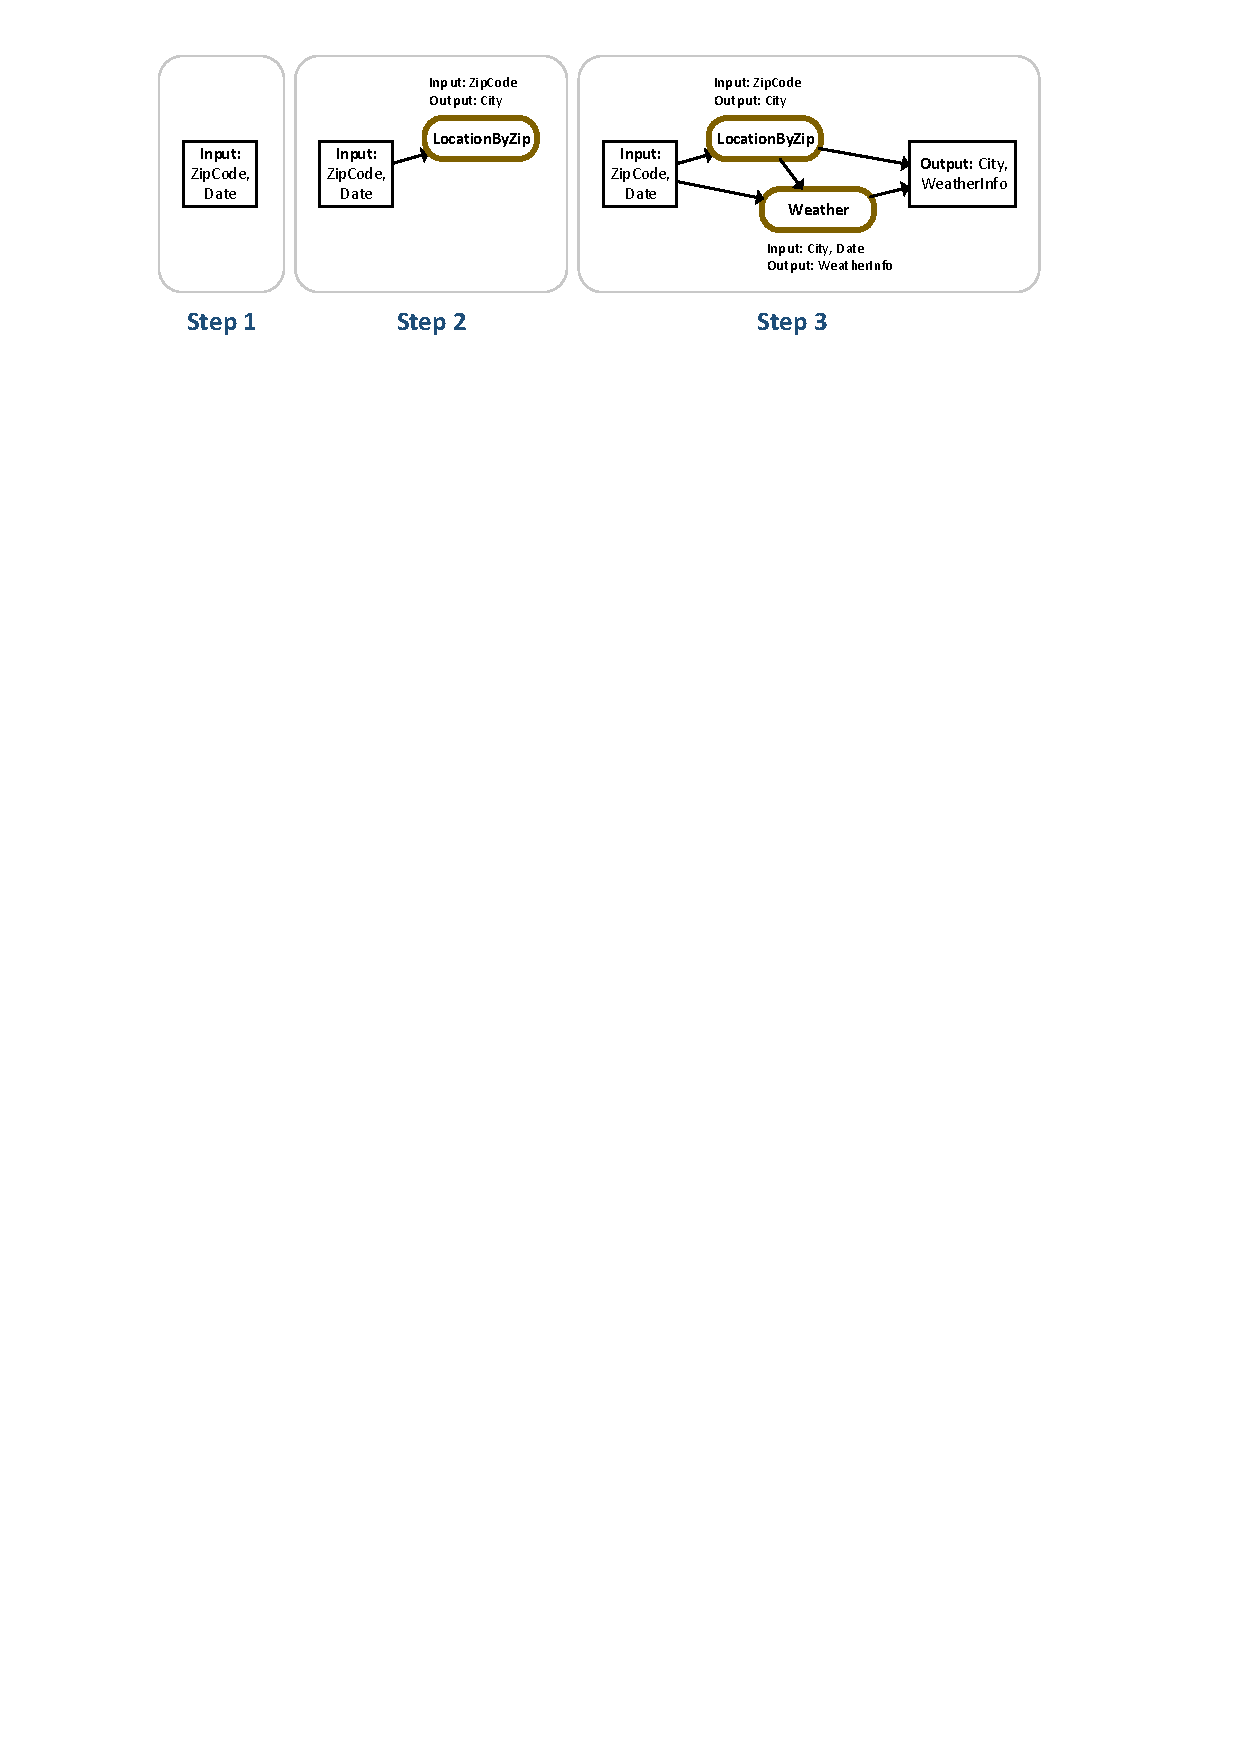
\includegraphics[width=14cm]{graphplan.pdf}
%}}
%\caption{Basic example of Web service composition using the Graphplan algorithm.}
%\label{fig:graphplan}
%\end{figure}

%In \cite{chen2014qos}, authors combine a planning algorithm and a graph search algorithm to achieve both QoS optimisation and feasibility in Web service compositions. The generic Graphplan algorithm first builds a representation of the search space as a planning graph, then finds a solution within this graph by traversing it backwards. This standard planning approach is modified to use Dijkstra's algorithm \cite{skiena1990dijkstra} when performing the backwards traversal, thus finding an optimised solution. The planning graph is extended to include labels associated with each proposition (i.e. each intermediate action between two vertices), where each label contains a layer number and associated execution costs. Dijkstra's algorithm is used to calculate the upcoming costs of each node in the graph. Then, a backtracking algorithm uses this information to determine the optimal solution.

%The work in \cite{deng2013efficient} proposes a planning-graph approach to creating a Web service composition technique that is capable of identifying the top K solutions with regards to overall QoS values. According to authors, AI planning is highly suitable to the domain of service composition, however many planning approaches are not efficiently executed. A notable exception to this trend is the planning-graph method, where the search space is greatly reduced through an initial search, thus allowing the remainder of the algorithm to focus on the relevant areas of the search space. In this work, the planning-graph approach is employed in a three-part algorithm. In the first part, a forward search is executed from the input node aiming to find the output node, gradually filtering the services that could be used in the composition. In the second part, the optimal local QoS of each service in the remaining graph is calculated using functions that take into consideration the QoS of the services that could possibly feed its input, also executed from the input node towards the output. Finally, a backward search algorithm is executed to generate the top K solutions according to local values calculated in the previous step (a threshold is provided when running this algorithm to prune out the substandard composition options).

%An automated Web service composition approach that uses a filtering algorithm to reduce the number of services considered for the composition, organising the remaining services as a graph according to the ways in which their inputs and outputs match, is proposed in \cite{huang2009effective}. Once the graph has been determined, a modified dynamic programming approach is applied to it in order to calculate the composition with the optimal QoS. Dynamic programming is a method that breaks problems into smaller subproblems that are then solved, ultimately leading to the solution of the parent problem. In this case, the optimal QoS of each atomic service in the graph is calculated, taking into account its input dependencies. At the end of this process, the overall optimal QoS values are known and the subgraph containing the solution can be extracted by searching the graph backwards. Experiments with the WSC2009 dataset show that the algorithm has good execution times for various dataset sizes, demonstrating its scalability. This work was extended in \cite{jiang2010qsynth}, with the presentation of a composition tool called QSynth, and the performance of formal comparisons with other state-of-the-art approaches, also producing superior results.

%A number of other works in the area employ formal AI planning techniques and frameworks to create compositions \cite{bertoli2009control}. The work in \cite{sohrabi2009web} presents an approach to include user preferences into the process of Web service composition. This is accomplished by relying on a framework written in Golog, a language created for agent programming. Golog is used to specify the particular attributes of generic workflows that represent commonly requested composition procedures (an example of a generic workflow would be one that is dedicated to booking inter-city transportation). The syntax of a logic-based language used to specify user preferences is described, allowing for branching according to conditions, and for expressing preferences over alternative services. Despite supporting branching, only one set of final outputs is allowed, meaning that the branches must be merged before reaching the end node of the composition workflow.

%An approach for modelling the data flow between Web services through the use of \textit{domain objects} is presented in \cite{kazhamiakin2013data}. For example, the travel domain contains objects such as flight ticket, hotel reservation, etc. The key idea is to use these objects to connect the composition needs to the services that can address them. In order to do so, authors annotate how each Web service operation relates to a given domain object. By creating this abstraction layer of objects, it is possible to reduce the composition's dependency on implementation details for correct execution. Now services can be thought of as having an object port proxy that leads to specific service ports. Compositions can then be achieved by identifying the necessary domain objects for the required task. The paper goes on to show how this technique can be integrated into existing service composition techniques, in this case AI-planning based, through the creation of a formal framework. This framework was implemented and run with a virtual travel agency scenario. According to the authors, the implementation of such framework was not trivial, however it successfully demonstrates that service implementations can be modified without impacting the overall composition.

%A Web service composition approach that allows users to specify constraints on the data flow of the solutions (i.e. which routes a message is allowed to take and which manipulations it can undergo) is presented in \cite{marconi2006specifying}. For example, consider a Web service composition that is supposed to book a holiday for a customer using a flights, accommodation, and a map service. If it is possible to book a suitable flight but it is not possible to book a hotel, the customer should not accept the offer. This is the type of requirement addressed by this approach using a data flow modelling language. This is a visual language that supports the definition of inputs/outputs, forking messages, merging messages, operations on messages, etc. By connecting these elements we obtain \textit{data nets} whose satisfiability can be clearly verified. The composition of Web services is performed using a planning framework that is capable of interpreting and respecting the constraints of a data net. At the time this paper was written, this approach had not yet been implemented or tested.

%\subsection{Hybrid Approaches}

%Hybrid approaches combine elements of AI planning and optimisation techniques for solving the composition problem with functionally correct, optimised solutions \cite{cotta2007memetic,pop2011tabu,xiang2011qos,chifu2012optimizing}. These hybrid approaches are quite similar to each other, relying on a directed acyclic graph as the base representation for a candidate solution, and then applying the optimisation techniques to this structure. However, despite incorporating the use of planning techniques, they do not include any discussion on the issue of producing solutions that satisfy conditional constraints or preferences. Another commonality between these works is that they require the use of SAWSDL-annotated datasets for testing, but these are not widely available to the research community. Therefore, authors developed their own datasets, and utilised each dataset's optimal task solution as the benchmark with which to evaluate the success of their implementation. More specifically, authors calculated the percentage of runs that culminated in the identification of the global optimum  as the recommended solution.

%In \cite{pop2010immune}, an approach that combines AI planning and an immune-inspired algorithm is used to perform fully automated QoS-aware Web service composition, also considering
%semantic properties. One significant contribution of this work is the proposal of an Enhanced Planning Graph (EPG), which extends the traditional planning graph structure
%by incorporating semantic information such as ontology concepts. Given this data structure, the composition algorithm selects the best solution configuration from a set of candidates. A fitness function considering QoS values and semantic quality is used to judge the best solution, and a clonal selection approach is employed to perform the optimisation. Candidates cells (solutions) are cloned, matured (mutated by replacing services with others from the same cluster in the EPG) and the cell most suited to combating the invading organism (i.e. the best solution) is discovered.

%The work in \cite{pop2011hybrid} proposes the employment of the Firefly meta-heuristic technique for performing QoS-aware Web service composition, in conjunction with an AI planning strategy that uses an EPG as the basis for solutions. The firefly meta-heuristic is based on the behaviour of mating fireflies, which emit a flashing light to attract potential mates. Each artificial firefly investigates the search space, with each position representing a composition solution. The brightness of the firefly is represented by the fitness of the current solution (location) associated with it. Fireflies are attracted to others according to their brightness, which varies with distance. Finally, fireflies move towards the individuals they are attracted to, meaning that small modifications occur in the current solution. The fitness function takes into account the QoS attributes of the composition.

%\section{Semantic Selection Approaches}\label{semantic}
%One important issue when creating compositions is that of selecting services that are compatible to each other. The simplest way of achieving this is by ensuring that the conceptual output and input types of any two services we wish to connect are perfectly matched, as illustrated by the Graphplan algorithm example in Section \ref{planning}. This involves accessing each service's WSDL, which is a formal description of a Web service's interface \cite{curbera2002unraveling}, and determining whether the two services offer compatible operations. However, in a more realistic scenario it may be very difficult to identify two services with such a precise fit. Because of this, an area of focus in the field of composition is that of semantic Web service selection. The fundamental idea of this approach is to annotate each service with additional semantic information so that the matching of services can be accomplished at a conceptual level. A well-known semantic standard for Web services is OWL-S (Web Ontology Language for Services) \cite{martin2007bringing} standard. OWL-S provides a formal specification of the workings of a service, allows for the association of conceptual classes with each Web service, and supports the use of ontologies that record the relationships between members of these different classes, thus establishing a common vocabulary for inter-service interactions. These features are conducive to automating the handling of Web services, and facilitating the discovery of those that are relevant for a specific task. Another more recent standard for semantic Web service annotation is SAWSDL (Semantic Annotations for WSDL) \cite{kopecky2007sawsdl}, a language that builds on WSDL by embedding pointers in the WSDL description that refer to semantic concepts. These pointers are called annotations, and are linked to concepts in a higher-level ontology layer.

%A number of different selection techniques that use semantic descriptions have been proposed recently \cite{soydan2004daml,wang2006qos,garcia2008qos,lin2008web,karakoc2009composing,boustil2010web,saboohi2011world,li2013towards,zhang2013genetic}. The work in \cite{DBLP:journals/soca/BoustilMS14}, for example, presents a selection strategy that considers more than just WSDL-level descriptions for Web services. In this approach, objects with additional information that is useful to the selection process are associated with each service. These objects have an independent ontology that describes how they interrelate (e.g. a service for making medical appointments has associated objects such as doctor, patient, hospital/clinic, etc), and at composition time the compatibility of these objects is verified. To accomplish this, a framework with service providers, ontology providers, information agents and a composer is proposed. This framework takes selection constraints set by the user into account.

%An automated semantic composition method is proposed in \cite{shin2007automated}. In this method, services are classified according to a functionality tag consisting of an \{action, object\} pair (e.g. a service for calculating the distance between two cities has the tag \{Calculate, Distance\}). A service relation graph is created to illustrate the dependencies between concepts, and it is divided in three parts: a graph showing relationships between actions, another graph showing relationships between objects (input/output relationships), and a mapping between items in these graphs. The relationships between these items are determined using domain ontology trees, with the assumption that these trees have already been provided. Given these dependencies, an algorithm is used to find a composition path. The path is found through the action graph and service connections are made based on the object graph, not only the object names. This approach was shown to require substantially less time to execute for larger datasets than previously proposed methods.

%The work in \cite{guo2010four} proposes a semantic Web service selection method that performs matching based on four distinct levels. At the \textit{Application Domain Matching} level the domain that best matches the user request is identified through the use of category ontologies, and a list of potential service description candidates is retrieved. This is performed by calculating a similarity degree between the user request and the semantic information associated with each domain. Subsequently, at the \textit{Service Description Matching} level, vectors are created for each potential service candidate description based on a given domain ontology, and another vector is created to represent the user requirements. A Vector Space Model is created, employing cosine similarity and TF-IDF to select the best service description. At the \textit{Service Function Matching} level, information from service providers is compared to the service description using a similarity measure, and a set of all services whose functionality fulfils the requirements is returned. Finally, at the \textit{QoS Matching} level, a matching array of quality values showing how closely a Web service matches the user's requirements is calculated, and the optimal candidate is returned.

%A framework for performing semantic Web service composition that also allows for user constraints to be specified is proposed in \cite{gamha2008framework}. Initially, services are grouped into distributed "service communities" according to their OWL-S semantic descriptions, where each community has services that cater for similar domains and consequently present similar functionalities. Then, users formulate their composition needs, including the necessary constraints, using terms from the semantic service community descriptions. Effectively, they create an abstract workflow for semi-automated composition by using the community descriptions and specifying their own preferences for the services to be selected. These constraints may be restrictions in input value ranges, in the output value ranges, or other service parameters. A language called KIF was chosen to express the constraints according to the corresponding OWL-S service descriptions. Interestingly, this approach can also handle world-altering services and non-deterministic functionality because it makes use of statecharts to model the behaviour of services.

%\section{Dynamic Web Service Composition}\label{dynamic}
%The approaches discussed thus far can be classified as static Web service composition, since they maintain a closed world assumption, that is, they assume that that the quality and the state of the services in the composition remains constant over time. However, in reality the state of the services available in a repository changes as time goes by, causing fluctuations in quality and even occasional failures. The area of dynamic Web service composition removes the closed world assumption, exploring solutions that can cope with quality fluctuations and service failures \cite{alferez2013facing,berg2013revenue,DBLP:journals/soca/WenTLCLH14}. The work in \cite{khakhkhar2012dynamic} proposes an algorithm that quickly creates a solution to satisfy a runtime service request, modelling the service composition problem as a graph in which a path is to be found. Forward and backward chaining approaches based on input/output matches are used for path exploration, relying on heuristics to encourage the exploration of the most promising paths and to reduce the number of services considered. In the approach proposed by this paper, both forward chaining and backward chaining are employed simultaneously, with the intention of having their paths meet in the middle. By doing so, the number of branches to be considered is greatly reduced. Experiments showed that the bidirectional search requires the exploration of a consistently smaller number of services when compared to the exclusively forward and exclusively backward approaches.

%A multi-objective Web service selection approach that optimises solutions according to two functions, a static one that calculates the overall quality of service (QoS) of a solution, and a dynamic one which calculates the \textit{trust degree} of a solution at a given time, is presented in \cite{wang2014novel}. The trust degree is defined as the number of successful executions of a service over its total number of executions, a piece of information that can be obtained by analysing execution logs. The optimisation algorithm used in this approach is an adaptive form of ant colony optimisation (ACO), where pheromones are adjusted according to the trust degree (calculated anew at every iteration) and the QoS is used by each ant as the heuristic for choosing the next node to visit. Each node in the graph explored by the ants represents an abstract service, with multiple concrete service candidates which can provide that functionality. The algorithm works by generating a set of of solutions and then identifying its Pareto subset by comparing all solutions. The Pareto subset is used in the next iteration, for updating the path pheromones. A case study is presented, comparing the performance of adaptive ACO to that of of the standard ACO algorithm, with results showing that adaptive ACO has a higher accuracy percentage than the standard ACO.

%The notion of transactions can be associated with service compositions, where different transactional properties guarantee certain runtime behaviours in a dynamic environment. The work in \cite{el2010tqos} proposes a semi-automated Web service composition approach that not only takes the functionality and quality of the services into account, but also their transactional properties. In this work, transaction properties are defined as the behaviour of Web services when interacting with one another. Knowing the behaviour of Web services is important for estimating how reliable their execution is and which ones might require recovery strategies at runtime. A service is considered \textit{retriable} if it can terminate successfully after multiple invocations, \textit{compensatable} if there is another service that can semantically undo its effects, and \textit{pivot} if its effects cannot be undone once it is executed but if it fails there are no effects. The system takes an abstract workflow and a set of user preferences as its inputs, where the user preferences contain QoS weights and risk levels corresponding to the transitional requirements for the composition. Then, a planner engine assigns one concrete Web service to each abstract slot of the provided workflow. Whenever a service is assigned to a part of the workflow, its transactional properties influence any subsequent services, thus the risk must be recalculated along with the overall QoS. Experiments were run for various risk scenarios, and computation time was found to remain under 2 seconds even for the largest dataset (comprising 3602 atomic Web services), at the same time meeting user preferences.

%An approach to QoS-aware Web service composition that is focused on \textit{rebinding}, that is, deciding which concrete services to bind to each abstract task at runtime in order to take the current state of the environment into consideration, is presented in \cite{parejo2014qos}. This approach considers global QoS constraints (e.g. the overall composition price must be lower than 5), local QoS constraints (e.g. the individual price for a service must be no higher than 1), and service dependency constraints (e.g. as many services as possible should be used from the same provider). Two techniques are employed during the composition process: GRASP, which is used to construct initial solutions, and Path Relinking, which is used to perform improvement on these solutions. \textit{GRASP} (Greedy Randomized Adaptive Search Procedure) iteratively builds a \textit{valid} solution vector, adding one candidate to fulfil each solution slot at a time and ensuring that this candidate respects the pre-established user constraints. The order of candidate addition matters, so it is performed randomly each time. Once a valid solution has been built, GRASP identifies a list of replacement candidates for each task slot, including the most promising candidates while also respecting the constraints observed by the valid solution. \textit{Path Relinking} explores the neighbouring solutions of the initial valid solution, seeking to further improve it. To do so, it slowly modifies solutions by changing services from one task slot at a time. The objective function used in this paper encourages the improvement of QoS values at the same time it enforces the relevant user constraints.

%\section{Summary and Limitations}\label{summary}
%This chapter presented an overview of the recent research conducted on different aspects of the automated Web service composition problem. The first area explored was that of \textbf{single-objective composition}, which aims to create composite solutions with the best possible overall Quality of Service (QoS) by conducting optimisations according to an objective function. Different approaches have been attempted for this, including both traditional approaches such as Integer Linear Programming (ILP) and Evolutionary Computation (EC) approaches such as Genetic Programming (GP), though in certain cases traditional approaches may not scale well as the composition problems grow in complexity. One key limitation of single-objective composition approaches is that they neglect the issue of branching, that is, they do not allow the creation of solutions with multiple alternative outputs that may be produced depending on a condition. To overcome this problem, a new candidate representation that also encodes this form of conditional branching needs to be proposed.

%Another area discussed is that of \textbf{multi-objective, top-K, and many-objective composition}, where each QoS attribute is optimised separately, and a set of solutions presenting trade-offs between these different quality attributes is generated. Multi-objective approaches work best for optimisation problems that involve two or three independent dimensions, while many-objective approaches are capable of handling more than three of them; top-K aims to produce a predetermined number of solution options based on a ranking strategy. The optimisation of multiple independent objectives is complex and provides many possibilities for further exploration. One interesting problem is that of many-objective optimisation for SLA-aware Web service composition, which refers to the constrained optimisation of several independent objectives to reflect the minimum quality requirements of the composition requestor. Accomplishing this is particularly challenging when creating solutions with multiple output possibilities.

%A number of \textbf{AI planning-based composition} approaches are also presented in this chapter. Their fundamental idea is to build solutions step by step, adding one atomic service to the composition at a time and subsequently checking whether the overall desired output has now been produced. These approaches are conducive to ensuring that the generated solutions are feasible and also included conditional branches into the solution's workflow whenever necessary. Despite these advantages, it is difficult to globally optimise the quality of a solution produced through planning, since its components are not modified or improved once they have been selected. A promising strategy to overcome this problem would be to combine planning algorithms with a population-based approach for optimisation, though this avenue has not yet been significantly explored by researchers.

%The \textbf{semantic Web service selection} approaches examined in this chapter propose a more realistic way of selecting the atomic components of a composition. Instead of expecting the return values and parameter types of service operations to match perfectly, the closest possible output-input matches are calculated using semantic distance measurements. The limitation of most works in this area is that they restrict their selection technique to semi-automated composition, where it is assumed that a framework with abstract service slots that are to be filled by concrete atomic services has already been provided. In the case of composition approaches based on AI planning techniques, where the workflow is built as services are connected to the solution, more flexible semantic selection methods are necessary. This motivates further research in this area.

%Finally, this chapter focuses on the issue of \textbf{dynamic Web service composition}. In this type of composition a closed world is abandoned, meaning that the state of services is expected to change throughout time. This brings two main problems: firstly, when the quality of the services in a repository changes, a solution that was once optimised according to the previous quality measures may suddenly transform into a low-standard alternative; secondly, certain services may become unavailable, meaning that solutions which incorporate them are henceforth unusable. The dynamic composition approaches discussed in this chapter use a variety of self-healing and recovery techniques to adjust solutions according to these changes, however they do not rely on EC techniques for doing so. These techniques can quickly re-optimise the QoS of existing solutions and provide composition backups (i.e. other candidates in the population) in case of failure, thus making EC an interesting dynamic alternative.

%\chapter{Preliminary Work}\label{C:preliminary}

This chapter exhibits the two initial works for comprehensive quality-aware semantic Web service composition approach, which combines a hybridization of various techniques for optimising the quality of semantic matchmaking and quality of service. In particular,  One direct representation and another indirect representation are proposed in two premilitary works using a PSO-based approach and a GP-based approach respectively. Apart from that, composition solutions are represented in a DAG or a tree-like representation,  respectively, in the two approaches. These two works are discussed in the following sections.

\section{Problem Formalisation}\label{problemDes}

We consider a \emph{semantic Web service} (\emph{service}, for short) as a tuple $S =(I_{S}, O_{S}, $ $QoS_S)$ where $I_{S}$ is a set of service inputs that are consumed by $S$, $O_{S}$ is a set of service outputs that are produced by $S$, and $QoS_{S}=\{t_S, c_S, r_S, a_S\}$ is a set of non-functional attributes of $S$. The inputs in $I_{S}$ and outputs in $O_{S}$ are parameters modelled through concepts in a domain-specific ontology $\mathcal{O}$. The attributes $t_S, c_S, r_S, a_S$ refer to the response time, cost, reliability, and availability of service $S$, respectively. These four QoS attributes are most commonly used \cite{zeng2003quality}.

A \emph{service repository} $\mathcal{SR}$ is a finite collection of services supported by a common ontology $\mathcal{O}$. A \emph{service request} (also called \emph{composition task}) over $\mathcal{SR}$ is a tuple $T=(I_{T}, O_{T})$ where $I_{T}$ is a set of task inputs, and $O_{T}$ is a set of task outputs. The inputs in $I_{T}$ and outputs in $O_{T}$ are parameters described by concepts in the ontology $\mathcal{O}$.

%A service composition is commonly represented as a \emph{directed acyclic graph} (DAG). Its nodes correspond to the services in the composition. 
\emph{Matchmaking types} are often used to describe the level of a match between outputs and inputs \cite{paolucci2002semantic}: For concepts $a, b$ in $\mathcal{O}$ the \emph{matchmaking} returns $exact$ if $a$ and $b$ are equivalent ($a \equiv b$), $plugin$ if $a$ is a sub-concept of $b$ ($a \sqsubseteq b$), $subsume$ if $a$ is a super-concept of $b$ ($a \sqsupseteq b$), and $fail$ if none of previous matchmaking types is returned. In this paper we are only interested in robust compositions where only $exact$ and $plugin$ matches are considered, see \cite{lecue2009optimizing}. As argued in \cite{lecue2009optimizing} $plugin$ matches are less preferable than $exact$ matches due to the overheads associated with data processing. We suggest to consider the semantic similarity of concepts when comparing different $plugin$ matches.

\emph{Robust causal link} \cite{lecue2008optimizing} is a link between two matched services $S$ and $S'$, noted as $S \rightarrow S'$, if an output $a$ ($a \in {O_S}$) of $S$ serves as the input $b$ ($b \in {O_{S'}}$) of $S'$ satisfying either $a \equiv b$ or $a \sqsubseteq b$.  For concepts $a, b$ in $\mathcal{O}$ the \emph{semantic similarity} $sim(a, b)$ is calculated based on the edge counting method in a taxonomy like WorldNet or Ontology \cite{shet2012new}. This method has the advantages of simple calculation and good performance \cite{shet2012new}. Therefore, the \emph{matchmaking type} and \emph{semantic similarity} of a robust causal link can be defined as follow:
\begin{align}
\label{eq_link}
type_{link} = 
\begin{cases}
	1 & \text{ if $a\equiv b$ ($exact$ match)}\\
	p & \text{ if $a \sqsubseteq b$ ($plugin$ match)}
\end{cases}
,&&
sim_{link} = sim(a,b) = \frac{2N_c}{N_{a}+N_{b}}
\end{align}

\noindent with a suitable parameter $p, 0<p< 1$, and with $N_a$, $N_b$ and $N_c$, which measure the distances from concept $a$, concept $b$, and the closest common ancestor $c$ of $a$ and $b$ to the top concept of the ontology $\mathcal{O}$, respectively. However, if more than one pair of matched output and input exist from service $S$ to service $S'$, $type_{link}$ and $sim_{link}$ will take on their average values.

The \emph{semantic matchmaking quality} of the service composition can be obtained by aggregating over all robust causal links as follow:
\begin{align}
MT {=} \prod_{j=1}^{m} type_ {link_{j}}
,&&
SIM {=} \frac{1}{m}\sum_{j=1}^m sim_ {link_{j}}  
\end{align}

We consider two special atomic services $Start = (\emptyset, I_T, \emptyset )$ and $End  = (O_T, \emptyset, \emptyset)$ to account for the input and output requirements given by the composition task $T$, and add them to $\mathcal{SR}$. 

Given a service request $T=(I_T,O_T)$, we represent a service composition solution for $T$ with services $S_1,\ldots,S_n$  by a weighted DAG, $\gra=(V,E)$ with node set $V=\{Start, S_1, S_2, $ $\ldots, S_n, End\}$ and edge set $E = \{link_{1}, link_{2},... link_{m} \}$. Each edge $link$ is a \emph{robust causal link}.


We also use formal expressions as in \cite{ma2012formal} to represent service compositions. We use the constructors $\bullet$, $\parallel$, $+$ and $\ast$ to denote sequential composition, parallel composition, choice, and iteration, respectively. The set of \emph{composite service expressions} is the smallest collection $\mathcal{SC}$ that contains all atomic services and that is closed under sequential composition, parallel composition, choice, and iteration. That is, whenever $\cse_0,\cse_1,\ldots,\cse_d$ are in $\mathcal{SC}$ then $\bullet(\cse_1,\ldots,\cse_d)$, $\parallel(\cse_1,\ldots,\cse_d)$, $+(\cse_1,\ldots,\cse_d)$, and $\ast \cse_0$ are in $\mathcal{SC}$, too. Let $\cse$ be a composite service expression. If $\cse$ denotes an atomic service $S$ then its QoS is given by $QoS_S$.  Otherwise the QoS for $\cse$ can be obtained inductively as summarized in Table~\ref{tbl:QoS_Aggre}. Herein, $p_1,\ldots,p_d$ with $\sum\limits^d_{k=1}p_k=1$ denote the probabilities of the different options of the choice $+$, while $\ell$ denotes the average number of iterations.

\begin{table}[htb]
\centering
\caption{QoS calculation for a composite service expression $\cse$}
\begin{tabular}{l|l|l|l|l}
\hline
 $\cse=$       &$r_\cse=$                              &$a_\cse=$                              &$c_\cse=$                            &$t_\cse=$ \\ \hline
 $\bullet(\cse_1,\ldots,\cse_d)$      &$\prod\limits^d_{k=1}r_{\cse_k}$    &$\prod\limits^d_{k=1}a_{\cse_k}$    &$\sum\limits^d_{k=1}c_{\cse_k}$   &$\sum\limits^d_{k=1}t_{\cse_k}$  \\ \hline
 $\parallel(\cse_1,\ldots,\cse_d)$  &$\prod\limits^d_{k=1}r_{\cse_k}$    &$\prod\limits^d_{k=1}a_{\cse_k}$    &$\sum\limits^d_{k=1}c_{\cse_k}$   &$MAX \{ t_{\cse_k} | k \in \{ 1,...,d \} \}$\\ \hline
 $+(\cse_1,\ldots,\cse_d)$     &$\prod\limits^d_{k=1}p_k\cdot r_{\cse_k}$    &$\prod\limits^d_{k=1}p_k\cdot a_{\cse_k}$    &$\sum\limits^d_{k=1}p_k\cdot c_{\cse_k}$   &$\sum\limits^d_{k=1}p_k\cdot t_{\cse_k}$  \\ \hline
 $\ast \cse_0$         &${r_{\cse_0}}^\ell$  &${a_{\cse_0}}^\ell$  &$\ell\cdot c_{\cse_0}$ &$\ell\cdot t_{\cse_0}$ \\ \hline
\end{tabular}
\label{tbl:QoS_Aggre}
\end{table}

When multiple quality criteria are involved in decision making, the fitness of a solution can be defined as a weighted sum of all individual criteria using Eq. (\ref{eq_fitness}), assuming the preference of each quality criterion is provided by users.
\begin{equation}
\label{eq_fitness}
Fitness = w_1 \hat{MT} + w_2 \hat{SIM} + w_3 \hat{A} + w_4 \hat{R} + w_5(1 - \hat{T}) + w_6(1 - \hat{C})
\end{equation}
\noindent with $\sum_{k=1}^{6} w_k= 1$. We call this objective function the \emph{comprehensive quality model} for service composition.
The weights can be adjusted according to users' preferences. $\hat{MT}$, $\hat{SIM}$, $\hat{A}$, $\hat{R}$, $\hat{T}$, and $\hat{C}$ are normalised values calculated within the range from 0 to 1 using Eq. (\ref{eq_normal}). To simplify the presentation we also use the notation $(Q_1,Q_2,Q_3,Q_4,Q_5,Q_6) $ $= (MT,SIM,A,R,T,C)$. $Q_1$ and $Q_2$ have minimum value 0 and maximum value 1. The minimum and maximum value of $Q_3$, $Q_4$, $Q_5$, and $Q_6$ are calculated across all task-related candidates in the service repository $\mathcal{SR}$ using the greedy search in \cite{ma2015hybrid,da2016genetic}.

\begin{equation}
\label{eq_normal}
\hat{Q_k} = 
\begin{cases}
	\frac{Q_k - Q_{k, min}}{Q_{k, max} - Q_{k, min}} & \text{ if $k=1,\ldots,4$ and }Q_{k, max} - Q_{k, min} \neq 0,\\
	\frac{Q_{k,max} - Q_k}{Q_{k, max} - Q_{k, min}} & \text{ if $k=5,6$ and }Q_{k, max} - Q_{k, min} \neq 0,\\
	1 & \text{ otherwise}.
\end{cases}
\end{equation}

\noindent To find best possible solution for a given composition task $T$, our goal is to maximise the objective function in Eq. (\ref{eq_fitness}).


\section{PSO-based Approach to Comprehensive Quality-Aware Automated Semantic Web service Composition}\label{qswsc_approach}
\subsection{An Overview of our PSO-based Approach}\label{PSO_based_approach}
As PSO has shown promise in solving combinatorial optimisation problems, we propose a PSO-based approach to comprehensive quality-aware automated semantic Web service composition. Fig. \ref{overview} shows an overview of our approach consisting of four steps: 
\begin{figure}[h]
\centering
\fbox{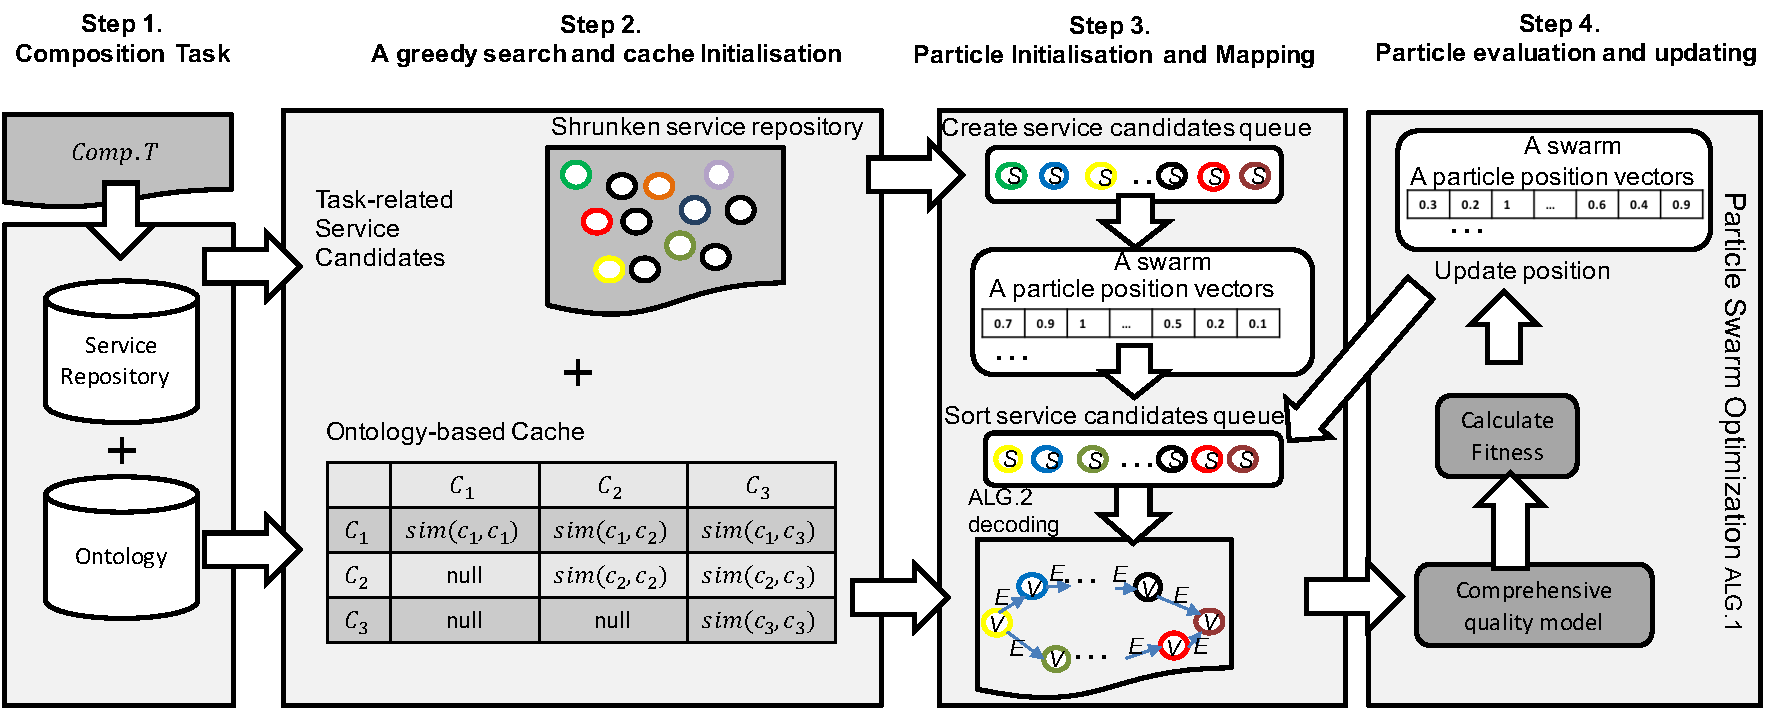
\includegraphics[scale=.5]{overview.pdf}}
 \caption{An overview of our PSO-based approach to comprehensive quality-aware automated semantic Web service composition.}
 \label{overview}
\end{figure}

Step 1: The composition process is triggered by a composition task, which is clearly defined in Section \ref{problemDes}. 

Step 2: The composition task is used to discover all task-related service candidates using a greedy search algorithm adopted from \cite{ma2015hybrid}, which contributes to a shrunken service repository. This greedy search algorithm keeps adding outputs of the invoked services as available outputs (initialised with $I_{T}$) , and these available outputs are used to discover task-related services from a service repository and updated with the outputs of these discovered services. This operation is repeated until no service is satisfied by the available outputs. During the greedy search, an ontology-based cache ($cache$) is initialised, which stores the concept similarities of matched inputs and outputs of task-related candidates. This $cache$ is also used to discover services by checking whether $null$ is returned by given two output-related and input-related concepts.

Step 3 and Step 4: These two steps follow the standard PSO steps \cite{shi2001particle} except for some differences in particles mapping and decoding processes. In particular, these two differences are related to sorting a created service queue using service-to-index mapping for a particle' position vectors and evaluating the fitness of a particle after decoding this service queue into a $\gra$ respectively. Those differences are further addressed in Algorithms \ref{novelSteps} and \ref{graph_building} in Section \ref{PSO-based_algomargin}.
\subsection{The Algorithms for our PSO-based Approach}\label{PSO-based_algomargin}
The overall algorithm investigated here is made up of a PSO-based Web service composition technique (Algorithm \ref{novelSteps}) and a $\gra$ creating technique from a service queue (Algorithm \ref{graph_building}). In Algorithm \ref{novelSteps}, the  steps $4$, $5$, $6$ and $7$ are different from those of standard PSO: In step 4, the size of task-related service candidates generated by a greedy search determines the size of each particle's position. Each service candidate in a created service candidates queue is mapped to an index of a particle’s position vectors, where each vector has a weight value between 0.0 and 1.0. In step 5, service candidates in the queue are sorted according to their corresponding weight values in descending order. In step 6, this sorted queue is used as one of the inputs of the forward decoding Algorithm \ref{graph_building} to create a $\gra$. In step 7, the fitness value of the created $\gra$ is the fitness value of the particle calculated by the comprehensive model discussed in Section \ref{problemDes}.
\begin{algorithm}
 %\LinesNumbered
 \SetKwInOut{Input}{Input}\SetKwInOut{Output}{Output}
 \SetKwFunction{generateWeightedGraph}{generateWeightedGraph}
 \SetKwProg{Procedure}{Procedure}{}{}
 \SetNlSty{}{}{:}
 Randomly initialise each particle in the swarm\;
  \While {max. iterations not met}{
     \ForEach{particle in the swarm}{
     Create a service candidates queue and map service candidates to a particle's position vectors\;
     Sort the service queue by position vectors' weights\;
     Use Algorithm \ref{graph_building} to create a $\gra$ from the service queue\;
     Calculate the $\gra$ fitness value\;
     
      \eIf{fitness value better than pBest}{    
        Assign current fitness as new \emph{pBest}\;
       }{
        Keep previous \emph{pBest}\;
       }	
     }
    Assign best particle's \emph{pBest} value to \emph{gBest}, if better than \emph{gBest}\;
 	Calculate the velocity of each particle\;
  	Update the position of each particle\;
  }
\caption{Steps of PSO-based service composition technique \cite{da2016particle}.}
\label{novelSteps}
\end{algorithm} 

Algorithm  \ref{graph_building} is a forward graph building algorithm extended from \cite{blum1997fast}. This algorithm takes one input, a sorted service queue from step 5 of Algorithm \ref{novelSteps}. Note that different service queues may lead to different $\gra$s. In addition. $I_{T}$, $O_{T}$ and $cache$ are also taken as the inputs. Firstly, $Start$ and $End$ are added to $V$ of $\gra$ as an initialisation, and $OutputSet$ is also created with $I_{T}$. The following steps are repeated until $O_{T}$ can be satisfied by $Outputset$ or the service queue is $null$. If all the inputs $I_{S}$ of the first popped  $S$ from $queue$ can be satisfied by provided outputs from $OutputSet$, this $S$ is added to $V$ and its outputs are added to $OutputSet$, and $S$ is removed from $queue$. Otherwise, the second popped  $S$ from $queue$ is considered for these operations. Meanwhile, $link$ is created with $type_{link}$ and $sim_{link}$ if $S$ is added, and calculated using information provided from $cache$. This forward graph building technique could lead to more services and edges connected to the $\gra$, these redundancies should be removed before $\gra$ is returned.

\begin{algorithm}
 \SetKwInOut{Input}{Input}\SetKwInOut{Output}{Output}
 \SetKwFunction{createWeightedDAG}{createWeightedDAG}
 \SetKwProg{Procedure}{Procedure}{}{}
 %\LinesNumbered
 \SetNlSty{}{}{:}
 % \Procedure{}{
 \Input{ $I_T$, $O_T$, $queue$, $cache$}
 \Output{$\gra$}
 $\gra = (V, E)$\;
 $V \leftarrow$ \{$Start$, $End$ \}\;
 $OutputSet \leftarrow$ \{$I_{T}$\}\;
  \While { $O_{T}$ not satisfied by $OutputSet$}{
     \ForEach{$S$ in $queue$}{
      \uIf{$I_{S}$ satisfied by $OutputSet$}{  
        insert $S$ into $V$\;  
        adjoin $O_{S}$ to $OutputSet$\;
        $queue$.remove $S$\;   
        $link \leftarrow$ calculate $type_{link}$, $sim_{link}$ using $cache$\;
        insert $link$ into $E$\;
       }	
     }
  }
 remove $dangling$ $nodes$ and $edges$ from $\gra$\; 
 \KwRet $\gra$\;
 %}
 \caption{Create a $\gra$ from a sorted service queue.}
\label{graph_building}
\end{algorithm} 

\section{Experiment Study for PSO-based Approach}\label{experiment_design}
In this section, we employ a quantitative evaluation approach with a benchmark dataset used in \cite{ma2015hybrid,da2016genetic}, which is an augmented version of Web service Challenge 2009 (WSC09) including QoS attributes. Two objectives of this evaluation are to: $(1)$ evaluate the effectiveness of our PSO-based approach, see comparison test in Section \ref{comparisonTestWithGP}. $(2)$ evaluate the effectiveness of our proposed comprehensive quality model to achieve a desirable balance on semantic matchmaking quality and QoS, see comparison test in Section \ref{comparisonTest}.

The parameters for the PSO are chosen from the settings from \cite{shi2001particle}, In particular, PSO population size is 30 with 100 generations. We run 30 times independently for each dataset. We configure the weights of fitness function to properly balance semantic matchmaking quality and QoS. Therefore, $w_{1}$ and $w_{2}$ are set equally to 0.25, and $w_{3}$, $w_{4}$, $w_{5}$, $w_{6}$ are all set to 0.125. The $p$ of $type_{link}$ is set to 0.75 ($plugin$ match) according to \cite{lecue2009optimizing}. In general, weight settings and parameter $p$ are decided according to users' preferences.

\subsection{GP-based vs. PSO-based approach}\label{comparisonTestWithGP}
To evaluate the effectiveness of our proposed PSO-based approach, we compare our PSO-based method with one recent GP-based approach \cite{ma2015hybrid} using our proposed comprehensive quality model. We extend this GP-based approach by measuring the semantic matchmaking quality between parent nodes and children nodes. To make a fair comparison, we use the same number of evaluations (3000 times) for these two approach. We set the parameters of that GP-based approach as 30 individuals and 100 generations, which is considered to be proper settings referring to \cite{da2015gp}.

The first column of Table \ref{meanFitness} shows five tasks from WSC09. The second and third column of Table \ref{meanFitness} show the original service repository size and the shrunk service repository size after the greedy search respectively regarding the five tasks. This greedy search helps reducing the original repository size significantly, which contributes to a reduced searching space. The fourth and fifth column of Table \ref{meanFitness} show the mean fitness values of 30 independent runs accomplished by two methods. We employ independent-samples T tests to test the significant differences in mean fitness value. The results show that the PSO-based approach outperforms the existing GP-based approach in most cases except Task 3. Note that all $p$-values are consistently smaller than 0.01. Using our PSO-based approach, small changes to sorted queues (particles in PSO) could lead to big changes to the composition solutions. This enables the PSO-based approach to escape from local optima more easily than the GP-based approach. 
%the PSO-based approach performs significantly better than the GP-based approach in finding optimal solutions. It may be that the GP-based approach is stuck in local optima in a very large search space due to its evolutionary operators. On the other hand, the decoding process used by the PSO-based approach allows for small changes that more effectively prevent this from happening.
\begin{table}[]
\centering
\caption{Mean fitness values for comparing GP-based approach}
\label{meanFitness}
\begin{tabular}{c|c|c|l|l}
\hline
\multicolumn{1}{c|}{WSC09} &Original $\mathcal{SR}$  &Shrunken $\mathcal{SR}$   &PSO-based approach & GP-based approach  \\ \hline
Task 1                     &572            &80    &0.5592 $\pm$ 0.0128  $\uparrow$  &0.5207 $\pm$ 0.0208           \\ \hline
Task 2                     &4129           &140   &0.4701 $\pm$ 0.0011  $\uparrow$  &0.4597 $\pm$ 0.0029          \\ \hline
Task 3                     &8138           &153   &0.5504 $\pm$ 0.0128              &0.5679 $\pm$ 0.0234 $\uparrow$   \\ \hline
Task 4                     &8301           &330   &0.4690 $\pm$ 0.0017  $\uparrow$  &0.4317 $\pm$ 0.0097            \\ \hline
Task 5                     &15211          &237   &0.4694 $\pm$ 0.0008  $\uparrow$  &0.2452 $\pm$ 0.0369            \\ \hline
\end{tabular}
\end{table}

\subsection{Comprehensive Quality Model vs. QoS Model}\label{comparisonTest}

Recently, a QoS Model, $Fitness = w_1 \hat{A} + w_2 \hat{R} + w_3(1 - \hat{T}) + w_4(1 - \hat{C})$, where $\sum_{i=1}^{4} w_i = 1$, is widely used for QoS-aware Web service composition \cite{ma2015hybrid,da2016particle,da2015graphevol}. To show the effectiveness of our proposed comprehensive quality model, we compare the best solutions found by this QoS model and our comprehensive model using our PSO-based approach. We record and compare the mean values of both $SM$ ($SM = 0.5 \hat{MT} + 0.5 \hat{SIM}$) and $QoS$($QoS = 0.25 \hat{A} + 0.25 \hat{R} + 0.25(1 - \hat{T}) + 0.25(1 - \hat{C})$) of best solutions over 30 independent runs. To make the comparison informative, all these recorded values have been normalised from 0 to 1, and compared using independent-samples T tests, see Table \ref{decisionTable}. Note that p-values are consistently smaller than 0.001 in the results indicating significant differences in performance. 

In Table \ref{decisionTable}, the mean values of $QoS$ using QoS model are significantly higher than those using comprehensive quality model for Tasks 2, 3, 4 and 5. However, the mean value of $SM$ using the comprehensive quality model are significantly higher than those using the QoS model, while a slight trade-off in $QoS$ are observed in all tasks. In addition, our comprehensive model achieves a consistently higher comprehensive quality in terms of a combination of $SM$ and $QoS$, which is significantly better in Tasks 1, 2, 3 and 4. 
\begin{table}[]
\footnotesize
\centering
\caption{Mean values of $SM$, $QoS$ and sum of $SM$ and $QoS$ for QoS model and comprehensive quality model using PSO-based approach}
\label{decisionTable}
\begin{tabular}{c|c|l|l}
\hline
\multicolumn{2}{c|}{WSC09}              & \shortstack{QoS \\ Model}         &\shortstack{Comprehensive Quality \\ Model} \\ \hline
\multirow{3}{*}{Task1}  &$SM$      &0.5373 $\pm$ 0.0267               &0.5580 $\pm$ 0.0094 $\uparrow$ \\ \cline{2-4}
                        &$QoS$     &0.5574 $\pm$ 0.0156               &0.5604 $\pm$ 0.0164            \\ \cline{2-4}
                        &$SM+QoS$  &1.0947 $\pm$ 0.0423               &1.1184 $\pm$ 0.0258 $\uparrow$ \\ \hline
\multirow{3}{*}{Task2}  &$SM$      &0.4549 $\pm$ 0.0033               &0.4630 $\pm$ 0.0042 $\uparrow$ \\ \cline{2-4} 
                        &$QoS$     &0.4800 $\pm$ 0.0012 $\uparrow$    &0.4772 $\pm$ 0.0025            \\ \cline{2-4}
                        &$SM+QoS$  &0.9349 $\pm$ 0.0045               &0.9402 $\pm$ 0.0067 $\uparrow$           \\ \hline
\multirow{3}{*}{Task3}  &$SM$      &0.5538 $\pm$ 0.0082               &0.6093 $\pm$ 0.0054 $\uparrow$ \\ \cline{2-4} 
                        &$QoS$     &0.4940 $\pm$ 0.0013 $\uparrow$    &0.4913 $\pm$ 0.0009            \\ \cline{2-4}
                        &$SM+QoS$  &1.0478 $\pm$ 0.0095               &1.1006 $\pm$ 0.0063 $\uparrow$           \\ \hline
\multirow{3}{*}{Task4}  &$SM$      &0.4398 $\pm$ 0.0037               &0.4604 $\pm$ 0.0000 $\uparrow$ \\ \cline{2-4} 
                        &$QoS$     &0.4845 $\pm$ 0.0010 $\uparrow$    &0.4734 $\pm$ 0.0044            \\ \cline{2-4}
                        &$SM+QoS$  &0.9243 $\pm$ 0.0047               &0.9338 $\pm$ 0.0044 $\uparrow$           \\ \hline
\multirow{3}{*}{Task5}  &$SM$      &0.4580 $\pm$ 0.0065               &0.4639 $\pm$ 0.0013 $\uparrow$ \\ \cline{2-4} 
                        &$QoS$     &0.4764 $\pm$ 0.0005 $\uparrow$    &0.4750 $\pm$ 0.0007            \\ \cline{2-4}
                        &$SM+QoS$  &0.9344 $\pm$ 0.0070               &0.9389 $\pm$ 0.0020           \\ \hline
\end{tabular}
\end{table}
\subsection{Further Discussion}\label{discuss1}
To analyse the effectiveness of achieving a good comprehensive quality at the expense of slightly reduced QoS, we demonstrate two best solutions produced using Task 3 as an example. Fig. \ref{comparisontest} $(1)$ and $(2)$ show two weighted DAGs, $\gra_1$ and $\gra_2$, which have been obtained as the best service compositions solutions based on the QoS model and on the comprehensive quality model, respectively. Both $\gra$s have exactly the same service workflow structure, but some service vertices and edges denoted in red are different. To better understand these differences, we list the overall semantic matchmaking quality $SM$,  overall $QoS$ and semantic matchmaking quality $sm_{link_n}$ associated to these different edges in $\gra_1$ and $\gra_2$. (Note: $sm_{link_n} = 0.5type_{link_n} + 0.5 sim_{e_n}$), where $\Delta Q$ reveals the gain (positive $\Delta Q$) or a loss (negative $\Delta Q$) of the listed qualities for our comprehensive quality model. Therefore, we achieve a comprehensive quality gain (+0.1433), a result of a gain in semantic matchmaking quality (+0.1467) and a loss in $QoS$ (-0.0034). To understand the improvement of semantic matchmaking quality from these numbers, we pick up $link_4$ that is associated with the smallest $\Delta Q$. The $link_4$ of $\gra_1$ and $\gra_2$ has two different source nodes, $Ser1640238160$ and $Ser947554374$, and two the same $End$ nodes. $Ser1640238160$ and $Ser947554374$ are services with output parameters $Inst582785907$ and  $Inst795998200$ corresponds to two concepts $Con2037585750$ and $Con103314376$ respectively in the given ontology shown in Fig. \ref{comparisontest} $(4)$. As $Inst658772240$ is a required parameter of $End$, and related to concept $Con2113572083$, $Inst795998200$ is closer to the required output $Inst658772240$ than $Inst582785907$. Therefore,  $Ser947554374$ is selected with a better semantic matchmaking quality compared to $Ser1640238160$.
\begin{figure}[h]
\centering{
\fbox{
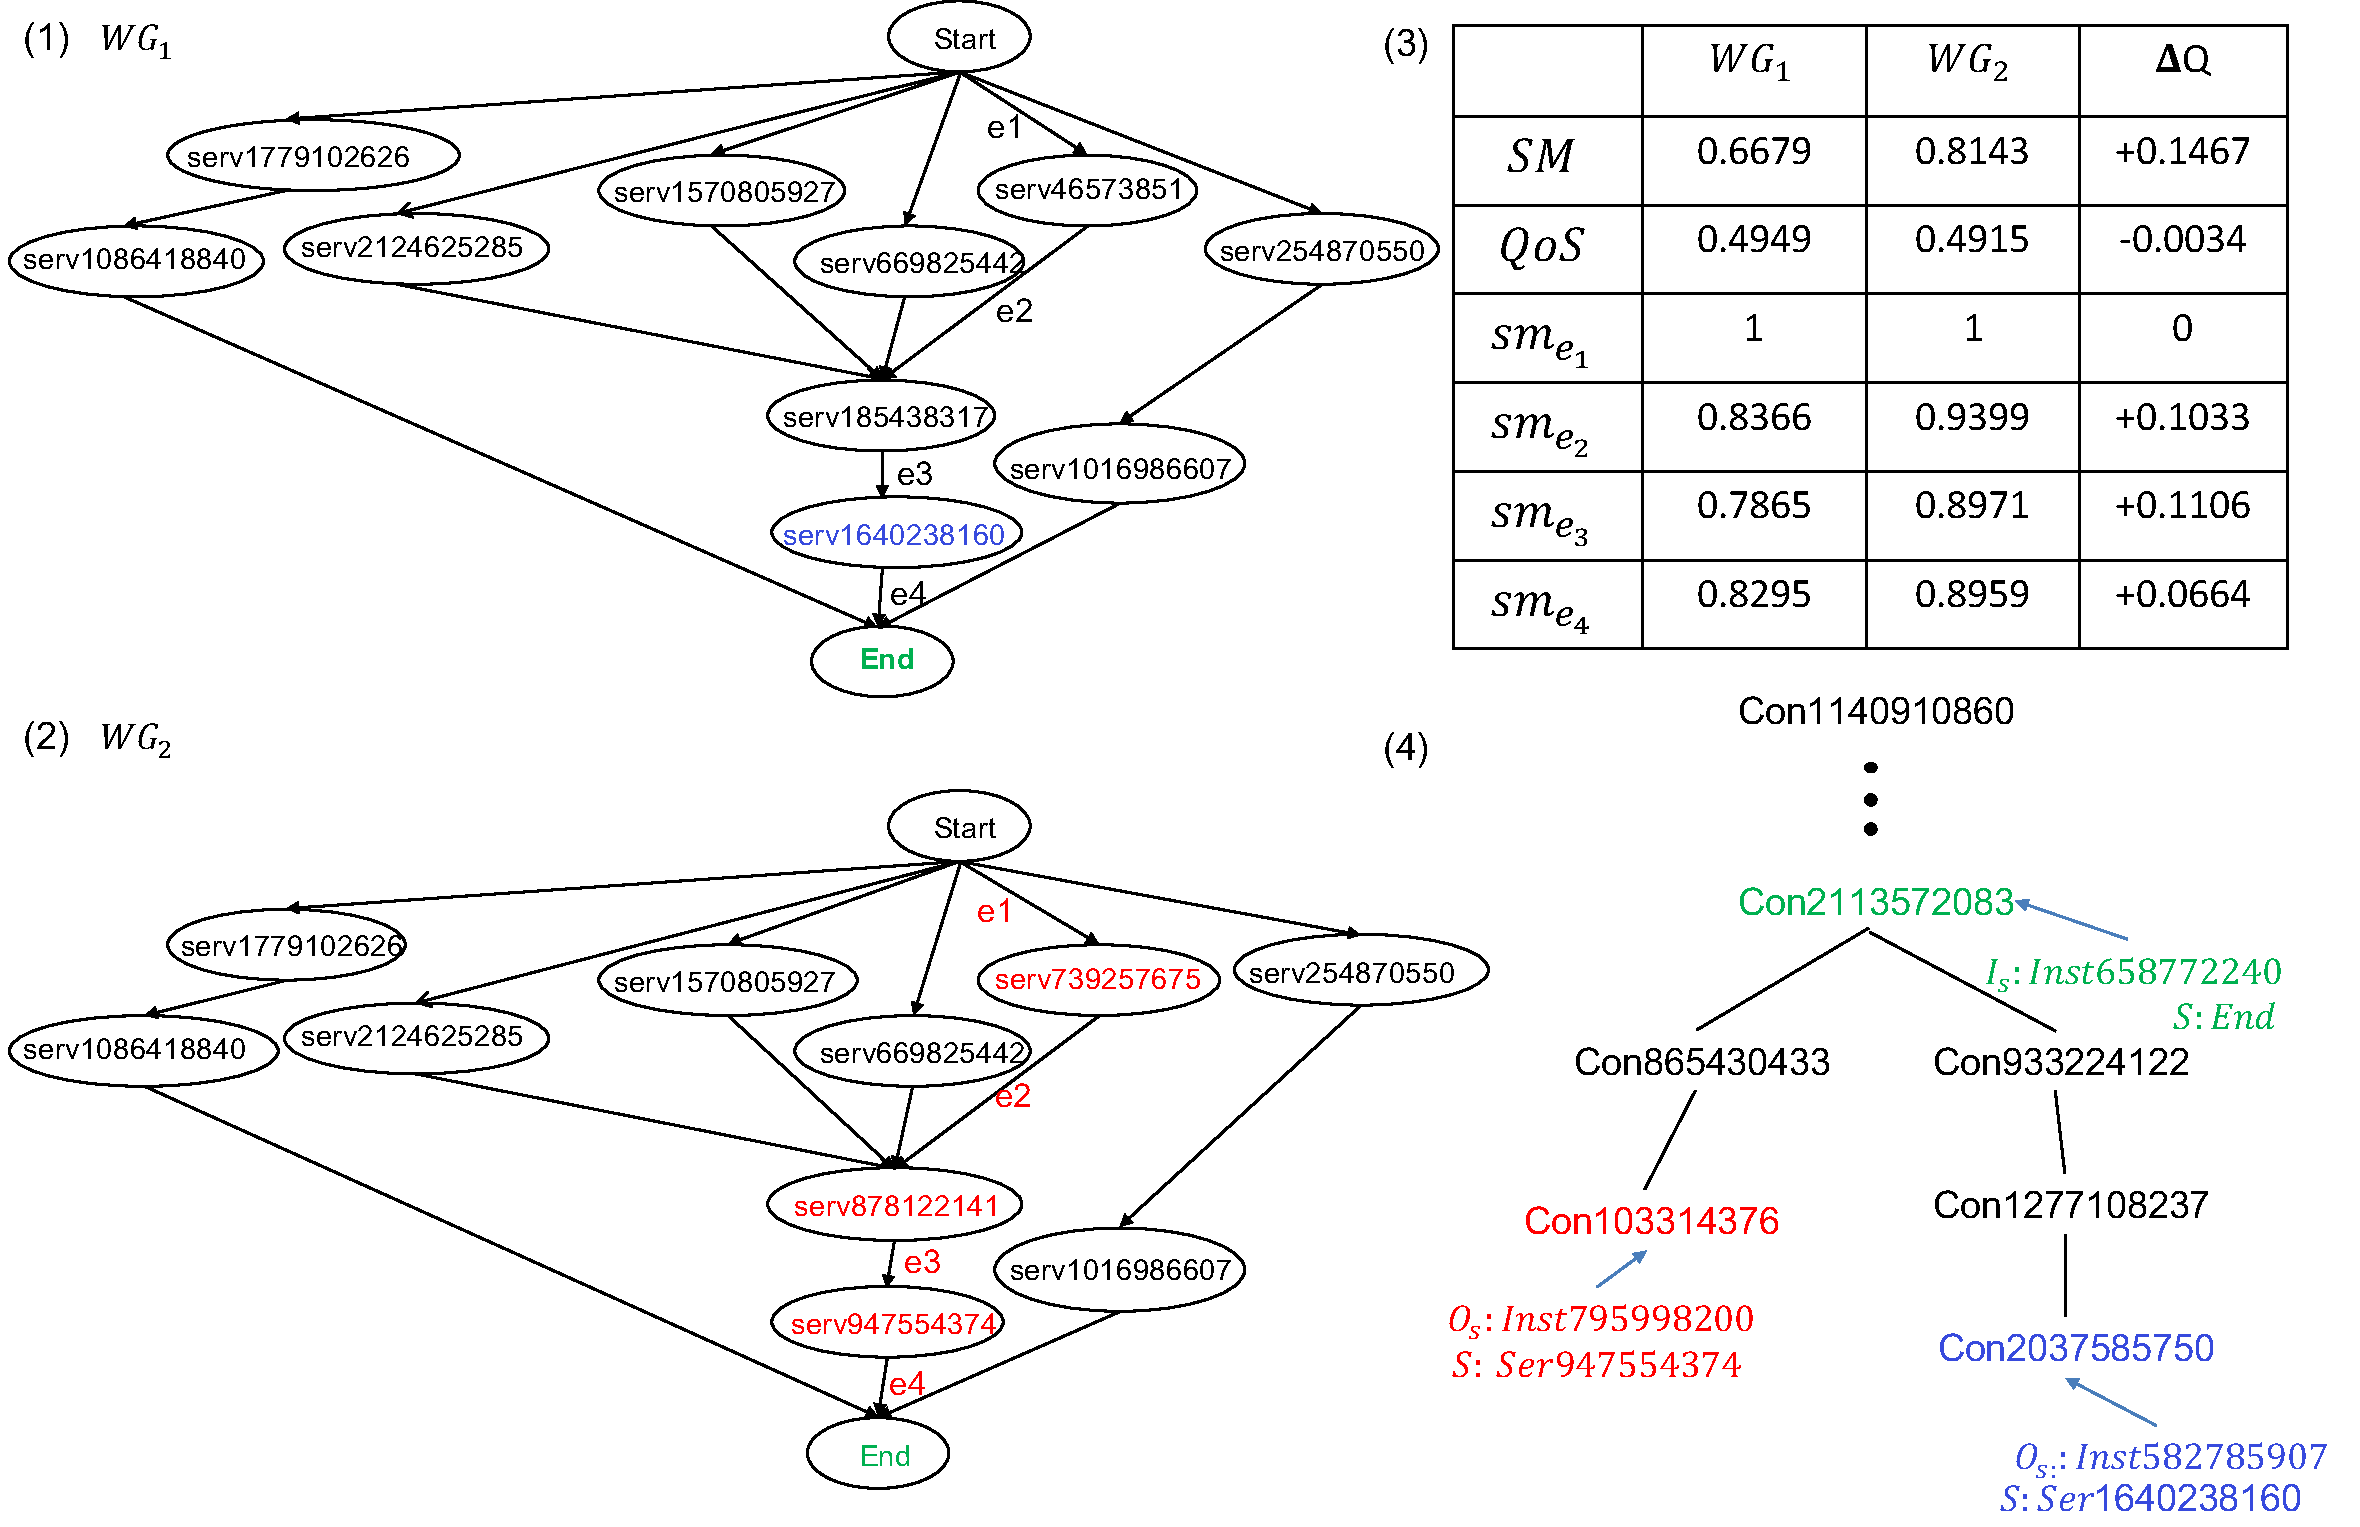
\includegraphics[scale=.29]{comparisontest.pdf}}}
 \caption{An example for the comparison of the best solutions obtained based on the QoS model and on the comprehensive quality model for Task 3.}
 \label{comparisontest}
\end{figure}

\section{Summary for our PSO-based Approach}\label{summary1}

In PSO-based approach, we propose an effective PSO-based approach to comprehensive quality-aware semantic Web service composition, which also has shown promise in achieving a better comprehensive quality in terms of a combination of semantic matchmaking quality and QoS compared to existing works.
%=================================================================================================== GP Approach
\section{GP-based Approach to Comprehensive Quality-Aware Automated Semantic Web service Composition}\label{GPApproach}

In this section, we first introduce the tree-like representation that will be used in our approach, and then discuss the differences to the most widely used tree-based representations for GP-based service composition in the literature \cite{gupta2015optimization,da2016genetic,yu2013adaptive}. Finally, we present our GP-based approach with newly designed genetic operation methods.
%========================================================================================= Representation
\subsection{A New Tree-like Representation for Web service Composition}\label{representation} 

Let $\gra=(V,E)$ be a weighted DAG representation of a service composition. Let $S$ be a service in $\gra$, and let $S_1,\ldots,S_d$ be its successors in $\gra$. We define the composite service expression relative to $S$ as follows: 
\begin{equation}
\label{eq_s_expression}
    \cse_S=
    \begin{cases}
      \bullet(S,\parallel(\cse_{S_1},\ldots,\cse_{S_d})), & \text{if $d\ge 2$}, \\
      \bullet(S,\cse_{S_1}), & \text{if $d=1$}, \\
      S, & \text{if $d=0$},
    \end{cases}
\end{equation}
which can be evaluated inductively starting with $Start$ which has no incoming edges in $\gra$. The resulting expression $C_{Start}$ is a composite service expression that is equivalent to $\gra$.
%Note: This needs to be modified slightly if there can be more nodes without incoming edges (other than Start). 

\begin{example}
Consider the composition task $T=(\{a, b, e\},\{ i\})$. Fig.~\ref{fig:ExampleOfRepresentation} shows an example of a composition solution. It involves four atomic services $S_1=(\{a, b \}, \{c, d, j \}, QoS_{S_1})$, $S_2=(\{c \}, \{f, g \}, QoS_{S_2})$, $S_3=(\{d \}, \{h \}, QoS_{S_3})$, and $S_4=(\{f, g, h \}, \{ i \}, QoS_{S_4})$. The two special services $Start=(\emptyset,\{a,b,e\},\emptyset)$ and $End=(\{i\},\emptyset,\emptyset)$ are defined by the given composition task $T$. The corresponding service composition expression is:

\noindent $\cse_{Start}=\bullet(Start,\bullet( S_1,\parallel(\bullet(S_2,\bullet(S_4,End)),\bullet(S_3,\bullet(S_4,End))))).$
\end{example}

Formal expressions can be visualized by expressions trees. For a composite service expression $\cse$ let $\tree$ denote the corresponding expression tree. 
%Let $V_t$ and $V_f$ denote the leaf nodes (also called \emph{terminal nodes}) and the internal nodes (also called \emph{functional nodes}) of $\tree$. 
Every leaf node in $\tree$ is labelled by the corresponding atomic service, while every internal node in $\tree$ is labelled by the corresponding composition constructor. For the sake of brevity we only consider $\bullet$ and $\parallel$ here, but our approach can easily be extended to $+$ and $\ast$, too. If a subtree of $\tree$ (except for $End$) has an isomorphic copy in $\tree$ then we remove it, label its root with a special symbol $q$, and insert an edge to the root of the copy. As a result we obtain a tree-like representation of a service composition. An example is shown in Fig.~\ref{fig:ExampleOfRepresentation}.

\begin{figure}[h!tb]
\centering
%\fbox{\includegraphics[scale=.30]{synthesisRules.pdf}}
\fbox{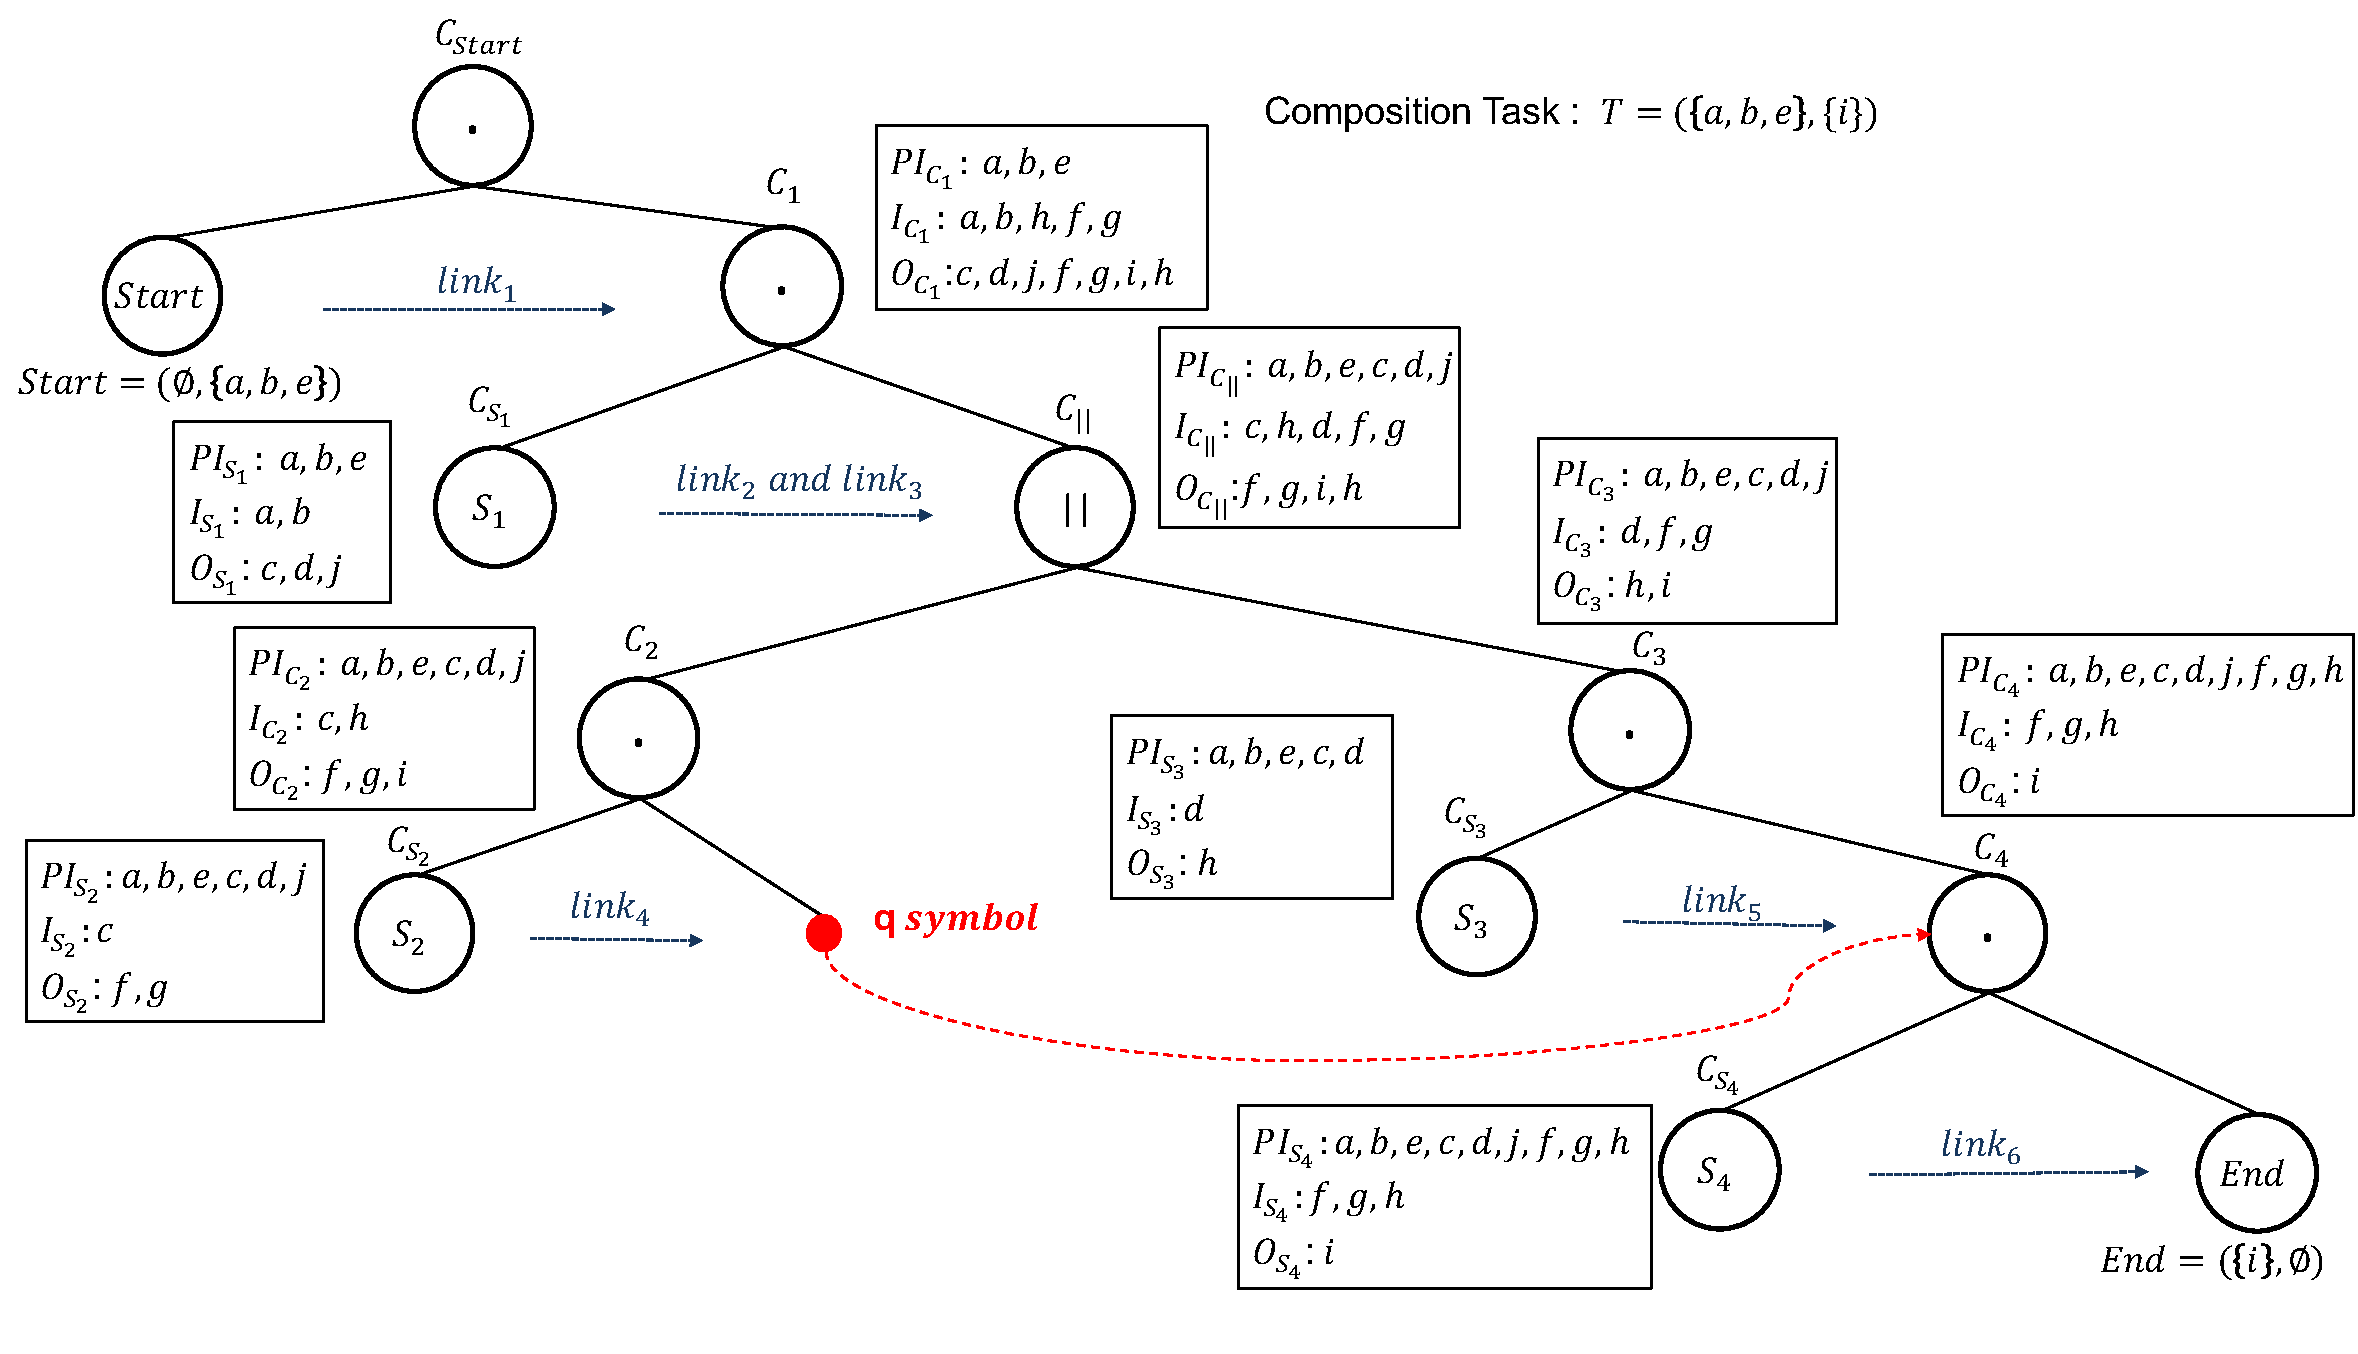
\includegraphics[width=1.0\textwidth]{Tree(p-symbol).pdf}}
 \caption{Example of a tree-like representation}
 \label{fig:ExampleOfRepresentation}
\end{figure}

%------------------- synthesis rules
Fig.~\ref{fig:ExampleOfRepresentation} shows for every atomic service $S$ its sets of (least required) inputs $\rin_S$ and outputs $\rout_S$. Moreover, the set of available inputs $\prin_S$ is shown which is just the union of the input sets of all (direct and indirect) predecessors of $S$ in the DAG.
%needs to be explained better
This can be easily generalized to composite service expressions. For a parallel composition $\cse=\parallel(\cse_1,\ldots,\cse_d)$ we define $\rin_\cse=\cup_{k=1}^d\rin_{\cse_k}$, and $\rout_\cse=\cup_{k=1}^d\rout_{\cse_k}$, and $\prin_\cse=\cup_{k=1}^d\prin_{\cse_k}$.
%we actually only need binary sequential compositions with a service in the first position
%not sure if this corresponds to what has been computed !!!
For a sequential composition $\cse=\bullet(S,\cse^\prime)$ we define $\rin_\cse=\rin_S\cup(\rin_{\cse^\prime}-\rout_S)$, and $\rout_\cse=\rout_S\cup\rout_{\cse^\prime}$, and $\prin_\cse=\prin_S$.
%more general we have:
%$\cse=\bullet(\cse_1,\ldots,\cse_d)$ we define $\rin_\cse=\rin_{\cse_1}\cup(\rin_{\cse_2}-\rout_{\cse_1})\cup\cdots\cup(\rin_{\cse_d}-\rout_{\cse_{d-1}})$ and $\rout_\cse=\rout_{\cse_1}\cup\cdots\cup \rout_{\cse_d}$, and $\prin_\cse=\prin_{\cse_1}\cup\cdots\cup \prin_{\cse_d}$. 

%------------------- new example
\begin{example}
%\cse here is actually \cse_{S_4}
Consider the sequential composition $\cse_4=\bullet(S_4, End)$ which is shown in the rightmost position in Fig.~\ref{fig:ExampleOfRepresentation}. We obtain $\rin_{\cse_4}=\{f, g, h\}$ which represents the (least required) inputs for this composition, and $\rout_{\cse_4}=\{i\}$ which represents the outputs produced by this composition, and $\prin_{\cse_4}=\{a, b, e, c, d, j, f, g, h\}$ which represents the union of the input sets of all (direct or indirect) predecessors of $S_4$ in the DAG (i.e., $S_1$, $S_2$ and $S_3$).
\end{example}

%\begin{example}
%Consider two atomic services $S_1$ with inputs $I_{S_1}=\{a,b\}$ and outputs $O_{S_1}=\{c,d\}$, and $S_2$ with inputs $I_{S_2}=\{c,d,e\}$ and outputs $O_{S_2}=\{f,g,h\}$. For their sequential composition $\cse=\bullet(S_1,S_2)$ we obtain $\rin_\cse=\{a,b,e\}$ which represents the least required inputs for this composition, $\rout_\cse=\{c,d,f,g,h\}$ which represents the outputs produced by this composition, and $\prin_\cse=\{a,b,e\}$ which represents the inputs that are provided by the predecessors of.
%this is not yet well described
%\end{example}

%\begin{figure}[h!tb]
%\centering
%%\fbox{\includegraphics[scale=.30]{synthesisRules.pdf}}
%\fbox{\includegraphics[width=.8\textwidth]{synthesisRules.pdf}}
% \caption{Example of representation and synthesis rules}
% \label{fig:ExampleOfSynthesisRules}
%\end{figure}

%Note that $\rin$, $\rout$ and $\prin$ can be computed recursively by tree traversal. For computing $\rin$ and $\rout$ we use pre-order depth-first traversal starting with the left-most leaf node of $Tree$, while for $\prin$ we use level-order breath-first traversal starting with the root node of $Tree$. 

%The representation used by our GP-based approach is a tree, $Tree = \{ V | \mathcal{R} \}$ with a set of nodes $V$ stored in a parent-child relationship $\mathcal{R}$ satisfying the following:
%\begin{enumerate}
%\item The node set $V = \{V_f,V_t\}$ consists of a set of functional nodes (internal nodes), $V_f = \{ \bullet, \parallel \}$, and a set of terminal nodes (leaf nodes), $V_t$=$\{Start, S_1, $ $S_2, \ldots, S_n, $ $End\}$. In $V_t$, $Start$ and $End$ are two special services defined as $Start = (\emptyset, I_T, \emptyset )$ and $End  = (O_T, \emptyset, \emptyset)$ that account for the input and output requirements given by the request $T$. 
 
%\item Each node $v \in V$ in $Tree$ is defined as a tuple $(I_{r}, O_{r}, I_{p}, QoS)$. The attributes $QoS$ are aforementioned in Sect. \ref{Problem Description}, while required inputs $I_r$, required outputs $O_r$ and provided inputs $I_p$ of $v$ are discussed here. $I_r$ is a set of inputs that is needed for executing the service composition represented in the subtree for which $v$ is the root node, and $O_r$ is obtained from the execution. $I_p$ of each $v \in V$ is a set of inputs available for $v$, which are obtained from two resources. One is from the task inputs $I_T$, and the other is from the outputs of $v$'s predecessor services in $Tree$, noted as $I_{pre}$.

%\item Some constrains are on $v \in V$ in $Tree$. The sequence node is always $\bullet(v_1 \in V_t, v_2 \in V)$ including two special cases for $Tree$'s $root$ and sequence constructs at the terminal level: $\bullet(Start, v_2 \in V_f)$ and $\bullet(v_1 \in V_t, End)$. The parallel node is always $\parallel(v_1\in V_f,..,v_n \in V_f)$, where $n\geq 2$.
%\end{enumerate}

Our representation supports composition constructs that are available in commonly used composition languages, such as BPEL4WS or OWL-S. Note that our representation is different from the most widely used tree-based representations in \cite{gupta2015optimization,da2016genetic,yu2013adaptive}. These differences are as follows.
\begin{enumerate}
\item $Start$ and $End$ are included in $\tree$, as they are related to measuring the semantic matchmaking qualities regarding $I_T$ and $O_T$.
\item $\rin_\cse$, $\rout_\cse$, $\prin_\cse$, $QoS_\cse$ are attributes, defined as a tuple $(\rin_\cse, \rout_\cse, \prin_\cse, QoS_\cse )$ for  any  $\cse_S$ in $\tree$. These attributes must be updated after population initialisation and genetic operations described in Sect. \ref{GP-Based Algorithm}.
\item $\tree$ preserves all the semantic matchmaking information, which can be easily used for computing robust casual links.
\end{enumerate}

%Based on and by extending the synthesis rules in \cite{fanjiang2014semantic}, we define a set of rules for computing $I_r$, $O_r$, $I_p$ of any $v \in V$ on $Tree$. The overall rules contain bottom-up and top-down methods to traverse $Tree$ recursively as follow: The bottom-up method for computing $I_r$, $O_r$ starts with the leftmost $v \in V_t$ in $Tree$ and continues to the right, then traverses the parent. On the other hand, the top-down method for calculating $I_p$ starts with the root of $Tree$, continues to traverse the children from the leftmost to the rightmost, then traverses the subtrees where each child is a root. During the traversal, $I_{r}$, $O_{r}$ and $I_{p}$ are updated in different ways according to each type of $v \in V_f$ as demonstrated in Fig. \ref{fig:ExampleOfSynthesisRules} $(b)$ and $(c)$. Note, for any $S(I_S, O_S) \in V_t$, $I_{r_{s}} = I_s$ and $O_{r_{s}} = O_s$.

%\begin{enumerate}
%\item If $v$ is $\bullet$, i.e.  $\bullet (S_1,S_2)$, when $S_1(\{a, b\}, \{c, d\}, QoS_1)$ and $S_2(\{c, d, e\}, \{f, g, h\}, $ $QoS_2)$, for $\bullet$, its $I_r = \{a, b, e \}$ is calculated by $I_{r_{1}} \cup (I_{r_{2}} \setminus  O_{r_{1}}) $, which presents the least required inputs for $\bullet$. Meanwhile, for $\bullet$, its $O_r = \{c, d, f, g, h \}$ is calculated by $O_{r_{1}} \cup O_{r_{2}}$, which presents all the output produced by $\bullet$. Suppose, for $\bullet$, its $I_{p}= \{a, b, e\}$ is inherited from the two resources ($I_T \cup I_{pre}$). For $S_1$, its $I_{p_{1}}= \{a, b, e\}$ as $I_{p}$ is passed to $S_1$. For $S_2$, its $I_{p_{2}} = \{a, b, e, c, d \}$ is calculated by $O_{r_{1}} \cup I_{p}$ as the both the inherited inputs produced $I_{p_{1}}$ and $O_{r_{1}}$ are included.

%\item If $v$ is $\parallel$, i.e. $\parallel(S_1,S_2)$, when $S_1(\{a, b\}, \{c, d\}, QoS_1)$ and $S_2(\{c, d, e\}, \{f,$ $ g, h\}, QoS_2)$, for $\parallel$, its $I_r = \{a, b, c, d, e \}$ is calculated by $ I_{r_{1}} \cup I_{r_{2}}$, which presents all the required inputs for $\parallel$. Meanwhile, for $\parallel$, its $O_r = \{c, d, f, g, h \}$ is calculated by $O_{r_{1}} \cup O_{r_{2}}$, which presents all the output produced by $\parallel$. Same as discussed above, for $\parallel$, its $I_{p} = \{a, b, e\}$ is inherited from the two resources ($I_T \cup I_{pre}$), For $S_1$ and $S_2$, $I_{p_{1}} = I_{p_{2}} = \{a, b, e\}$ as $I_{p}$ is passed to its children.
%\end{enumerate}


To compute semantic matchmaking quality, we need to retrieve all the robust causal links on $\tree$. This is performed by retrieving robust  causal links for every  sequential composition $\cse=\bullet(S,\cse^\prime)$. For example,  in Fig \ref{fig:ExampleOfRepresentation}, two robust causal links ($link_2: S_1 \rightarrow S_2$ and $link_3: S_1 \rightarrow S_3$ ) are retrieved from $\cse_1 = \bullet (S_1, \cse_{\parallel})$, because outputs $O_{S_1}=\{ c, d, j \}$ match inputs $I_{\cse_{\parallel}}=\{c, h, d, f, g\}$.


%\begin{algorithm}
% \setlength\hsize{0.9\linewidth}
% \SetKwInOut{Input}{Input}\SetKwInOut{Output}{Output}
% \SetKwFunction{evaluateSemanticLink}{evaluateSemanticLink}
% \SetKwProg{Procedure}{Procedure}{}{}
% \LinesNumbered
% \SetNlSty{}{}{:}
%  \Procedure{evaluateSemanticLink( ){}}{
% \Input{Tree $T$, IndexCache $cache$}
% \Output{Match type quality $MT$, Concept similarity $S$}
% \{ $ServNode \} \leftarrow  T.getAllServNode$\;
%     \ForEach{$ServNode$ in  \{ $ServNode$ \} }{
%      $NeighbourNode \leftarrow  ServNode.getNeighbourNode$\;
%    	 \ForEach{$O$ in $ServNode.outputs$ and $I$ in $NeighbourNode.requiredInputs$}{
%	  $mt_{P}, s_{P} \leftarrow$ query $cache(O,I)$\;
%	  $mt_{L} \leftarrow$ aggregation( $mt_{p}$ )\;
%	  $s_{L} \leftarrow$ aggregation( $s_{p}$ )\;
%	  \{$mt_{L}$ \} add $mt_{L}$\;
%	  \{$s_{L}$ \} add $s_{L}$\;
%        }
%       $MT \leftarrow$ aggregation( \{ $mt_{L}$\} )\;
%       $S \leftarrow$ aggregation( \{ $s_{L}$ \} )\;
%       }
% \KwRet $MT, S$\;
% }
% \caption{Evaluate semantic link in the tree.}
%\label{evaluateSemanticLink}
%\end{algorithm} 

%========================================================================================= Algorithm
\subsection{GP-Based Algorithm}\label{GP-Based Algorithm}

Now we present our GP-based approach for service composition, see Algorithm~\ref{GP-based algorithm}. To begin with the algorithm, we generate the initial population $P_0$, which is then evaluated using our comprehensive quality model. The iterative part of the algorithm comprises lines 3 to 7,  which will be repeated until the maximum number of generations is reached or the best solution is found. During each iteration, we use tournament selection to select individuals, on which crossover and/or mutation are performed to evolve the polulation. These steps correspond to the standard GP steps \cite{koza1992genetic} except for some particularities that will be discussed below.

%How do we know that we have found the best solution? In the algorithm below: where do we get max.fitness from?

\begin{algorithm}[h!tb]
 %\LinesNumbered
 \SetKwInOut{Input}{Input}\SetKwInOut{Output}{Output}
 \SetKwFunction{generateWeightedGraph}{generateWeightedGraph}
 \SetKwProg{Procedure}{Procedure}{}{}
 \SetNlSty{}{}{:}
 \Input{ $T$, $\mathcal{SR}$, $\mathcal{O}$}
 \Output{an optimal composition solution}
 Initialise population $P_0$ (using a 3-step method)\;
 Evaluate each individual in population $P_0$ (using our comprehensive quality model)\;
  \While {max.populations or max.fitness not yet met}{
     Select the fittest individuals for evolution\;
     Apply crossover and mutation to the selected individuals\;
%     Generate new individuals\;
     Evaluate each new individual\;
     Replace the individuals with the smallest fitness in the population by the new individuals\;
  }
 Find the individual with the highest fitness in the final population\;
\caption{GP-based algorithm for service composition.}
\label{GP-based algorithm}
\end{algorithm} 

\textbf{Population initialisation.}
The initial population is created by generating a set of service compositions in form of DAGs, and then transforming them into their tree-like representations (\emph{the individuals}). The initialisation is performed as follows: 

%Should we explain when a DAG is valid service composition solution?
\textsc{Step 1}. Greedy search is performed to randomly generate a set of DAGs, each representing a (valid) service composition for the given composition task $T$. For this, a simple forward graph building algorithm is applied starting with the node $Start$ and the inputs $I_T$ of the composition task $T$. Details of this algorithm can be found in \cite{ma2015hybrid}. An example of a generated DAG is shown in Fig.~\ref{fig:DAG} with seven robust casual links marked on.

\textsc{Step 2}. The DAGs can be simplified by removing some redundant edges and service nodes. 
%We formalise the criteria for identifying such edges: The outgoing edges from an atomic service $S$ to its direct successors are considered for removal if the direct successors overlap with their successors. This criterion is checked from $Start$ to $End$. 
While this step is not compulsory, it can help to notably reduce the size of the DAG and, consequently, the corresponding tree-like representation. 

\textsc{Step 3}. 
%For each DAG we initialize an auxiliary data structure to record the available inputs for every service node in the DAG. 
We transform each DAG into its tree-like representation using an algorithm modified from \cite{da2016genetic} to satisfy the particular requirements of our proposed approach. For example, Fig.~\ref{fig:ExampleOfRepresentation} shows an example of a tree-like individual corresponding to the DAG shown in Fig.~\ref{fig:DAG}.

%\begin{example}
%Fig.~\ref{DAG} illustrates the generation and simplification of a DAG.  The  corresponding tree shown in Fig.~\ref{fig:ExampleOfRepresentation} is transferred from this DAG. In the initial DAG, service $S_4$ requires the inputs produced by $S_1$, $S_2$ and $S_3$. However, $S_4$ can not be invoked until both $S_2$ and $S_3$ are executed. Therefore, we can simplify the DAG by removing the edge between $S_1$ and $S_4$ (noted as $link_7$) without impacting the execution of a service composition. To transform the DAG into a tree, we traverse the DAG from $Start$ to $End$ with a cursor to mark the current position while creating a node in the tree according to the cursor's position and the number of outgoing edges. In addition, seven robust casual links marked in this DAG could be retrieved from transferred tree in Fig.~\ref{fig:ExampleOfRepresentation} .
%\end{example}

\begin{figure}[htb]
\centering
%\fbox{\includegraphics[scale=.30]{transformationExample.pdf}}
\fbox{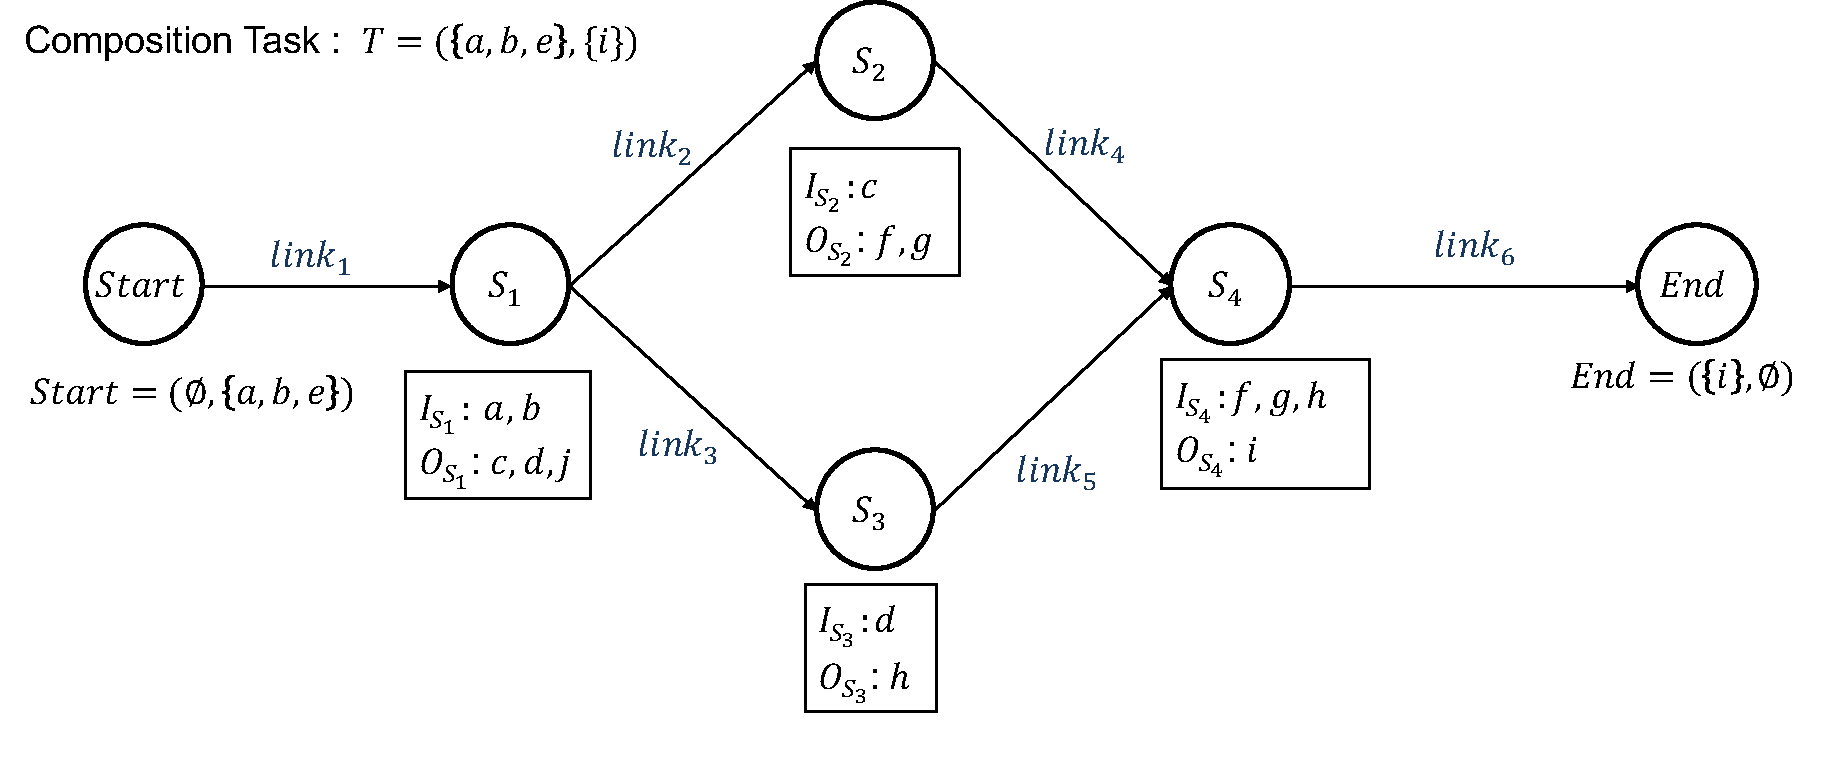
\includegraphics[width=.7\textwidth]{DAG(p-symbol).pdf}}
 \caption{Example of a weighted DAG used for transferring it into tree-like representation}
 \label{fig:DAG}
\end{figure}


%\begin{figure}[htb]
%\centering
%%\fbox{\includegraphics[scale=.30]{transformationExample.pdf}}
%\fbox{\includegraphics[width=.8\textwidth]{transformationExample.pdf}}
% \caption{Example for the transformation of the DAG for a service composition into its tree-like representation}
% \label{transformationExample}
%\end{figure}

%This section still needs to be modified. I can describe crossover and mutation similar to the GraphEvol approach (though these are a bit more restrictive than the crossover and mutation considered so far in this paper). Or I can describe it a bit more general or even leave it somewhat open.
%Later we need an example. The solution of Dataset 3 is a possible example, but a bit small. I would like to see the solution of Dataset 4 before I can say what a good example would be.
\textbf{Crossover and Mutation.} 
During the evolutionary process, the correctness of the representation is maintained by crossover and mutation. 

A crossover operation exchanges a subtree of a selected individual (its attributes noted as $\cse_1 (\rin_{\cse_1}, \rout_{\cse_1}, \prin_{\cse_1}, QoS_{\cse_1})$) with the subtree of another selected individual (its attributes noted as $\cse_2 (\rin_{\cse_2}, \rout_{\cse_2}, \prin_{\cse_2}, QoS_{\cse_2})$) 
if they represent the same functionality (i.e. $\rin_{\cse_1} = \rin_{\cse_2}$ and $\rout_{\cse_1} = \rout_{\cse_2}$). That is, at the root nodes of both subtrees, we have identical inputs and identical outputs. A crossover operation is performed in two cases: crossover on two functional nodes or on two terminal nodes. We never exchange a functional node with an terminal node, since the two associated subtrees cannot be equivalent in this case. For example, $End$ must appear in the subtree associated with any functional node, but not for any selected terminal node (atomic services). 
%\begin{figure}[h]
%\centering
%\fbox{\includegraphics[scale=.26]{crossoverExample.pdf}}
% \caption{Example of a crossover}
% \label{crossoverExample}
%\end{figure}

A mutation operation replaces a subtree of the selected individual (its attributes noted as $\cse_1 (\rin_{\cse_1}, \rout_{\cse_1}, \prin_{\cse_1}, QoS_{\cse_1})$) with a newly generated subtree satisfying the least required functionality. To do this, a subtree $\cse_1$ must be selected from the selected individual, and a new composition task $T=(\{\prin_{\cse_1}\},\{\rout_{\cse_1} \cap O_T\})$ or $T'=(\{\prin_{\cse_1}\},\{\rout_{\cse_1}\})$ is used to generate a tree in the same way as the 3-step method performed during the population initialisation. We utilise the available inputs and least required outputs for mutation, because it potentially bring more possibilities in generating more varieties of subtrees. The mutation is performed in two cases: mutation on a functional node with $T$ or on a service node with $T'$, two examples shown in Fig \ref{mutationExample} $(a)$ and $(b)$. In Fig \ref{mutationExample} $(a)$, a functional node $\cse_{\parallel}$ is selected for mutation, the whole subtree is replaced with the generated subtree excluding its head (i.e., $Start$ and its parent node $\bullet$). In Fig \ref{mutationExample} $(b)$, a atomic service $S_1$ is selected for mutation, the branch of the selected node (i.e., $S_1$ and its parent node $\bullet$) is replaced with the generated subtree excluding both its head (i.e., $Start$ and its parent node $\bullet$) and its tail (i.e., $End$).

\begin{figure}[h!tb]
\centering
%\fbox{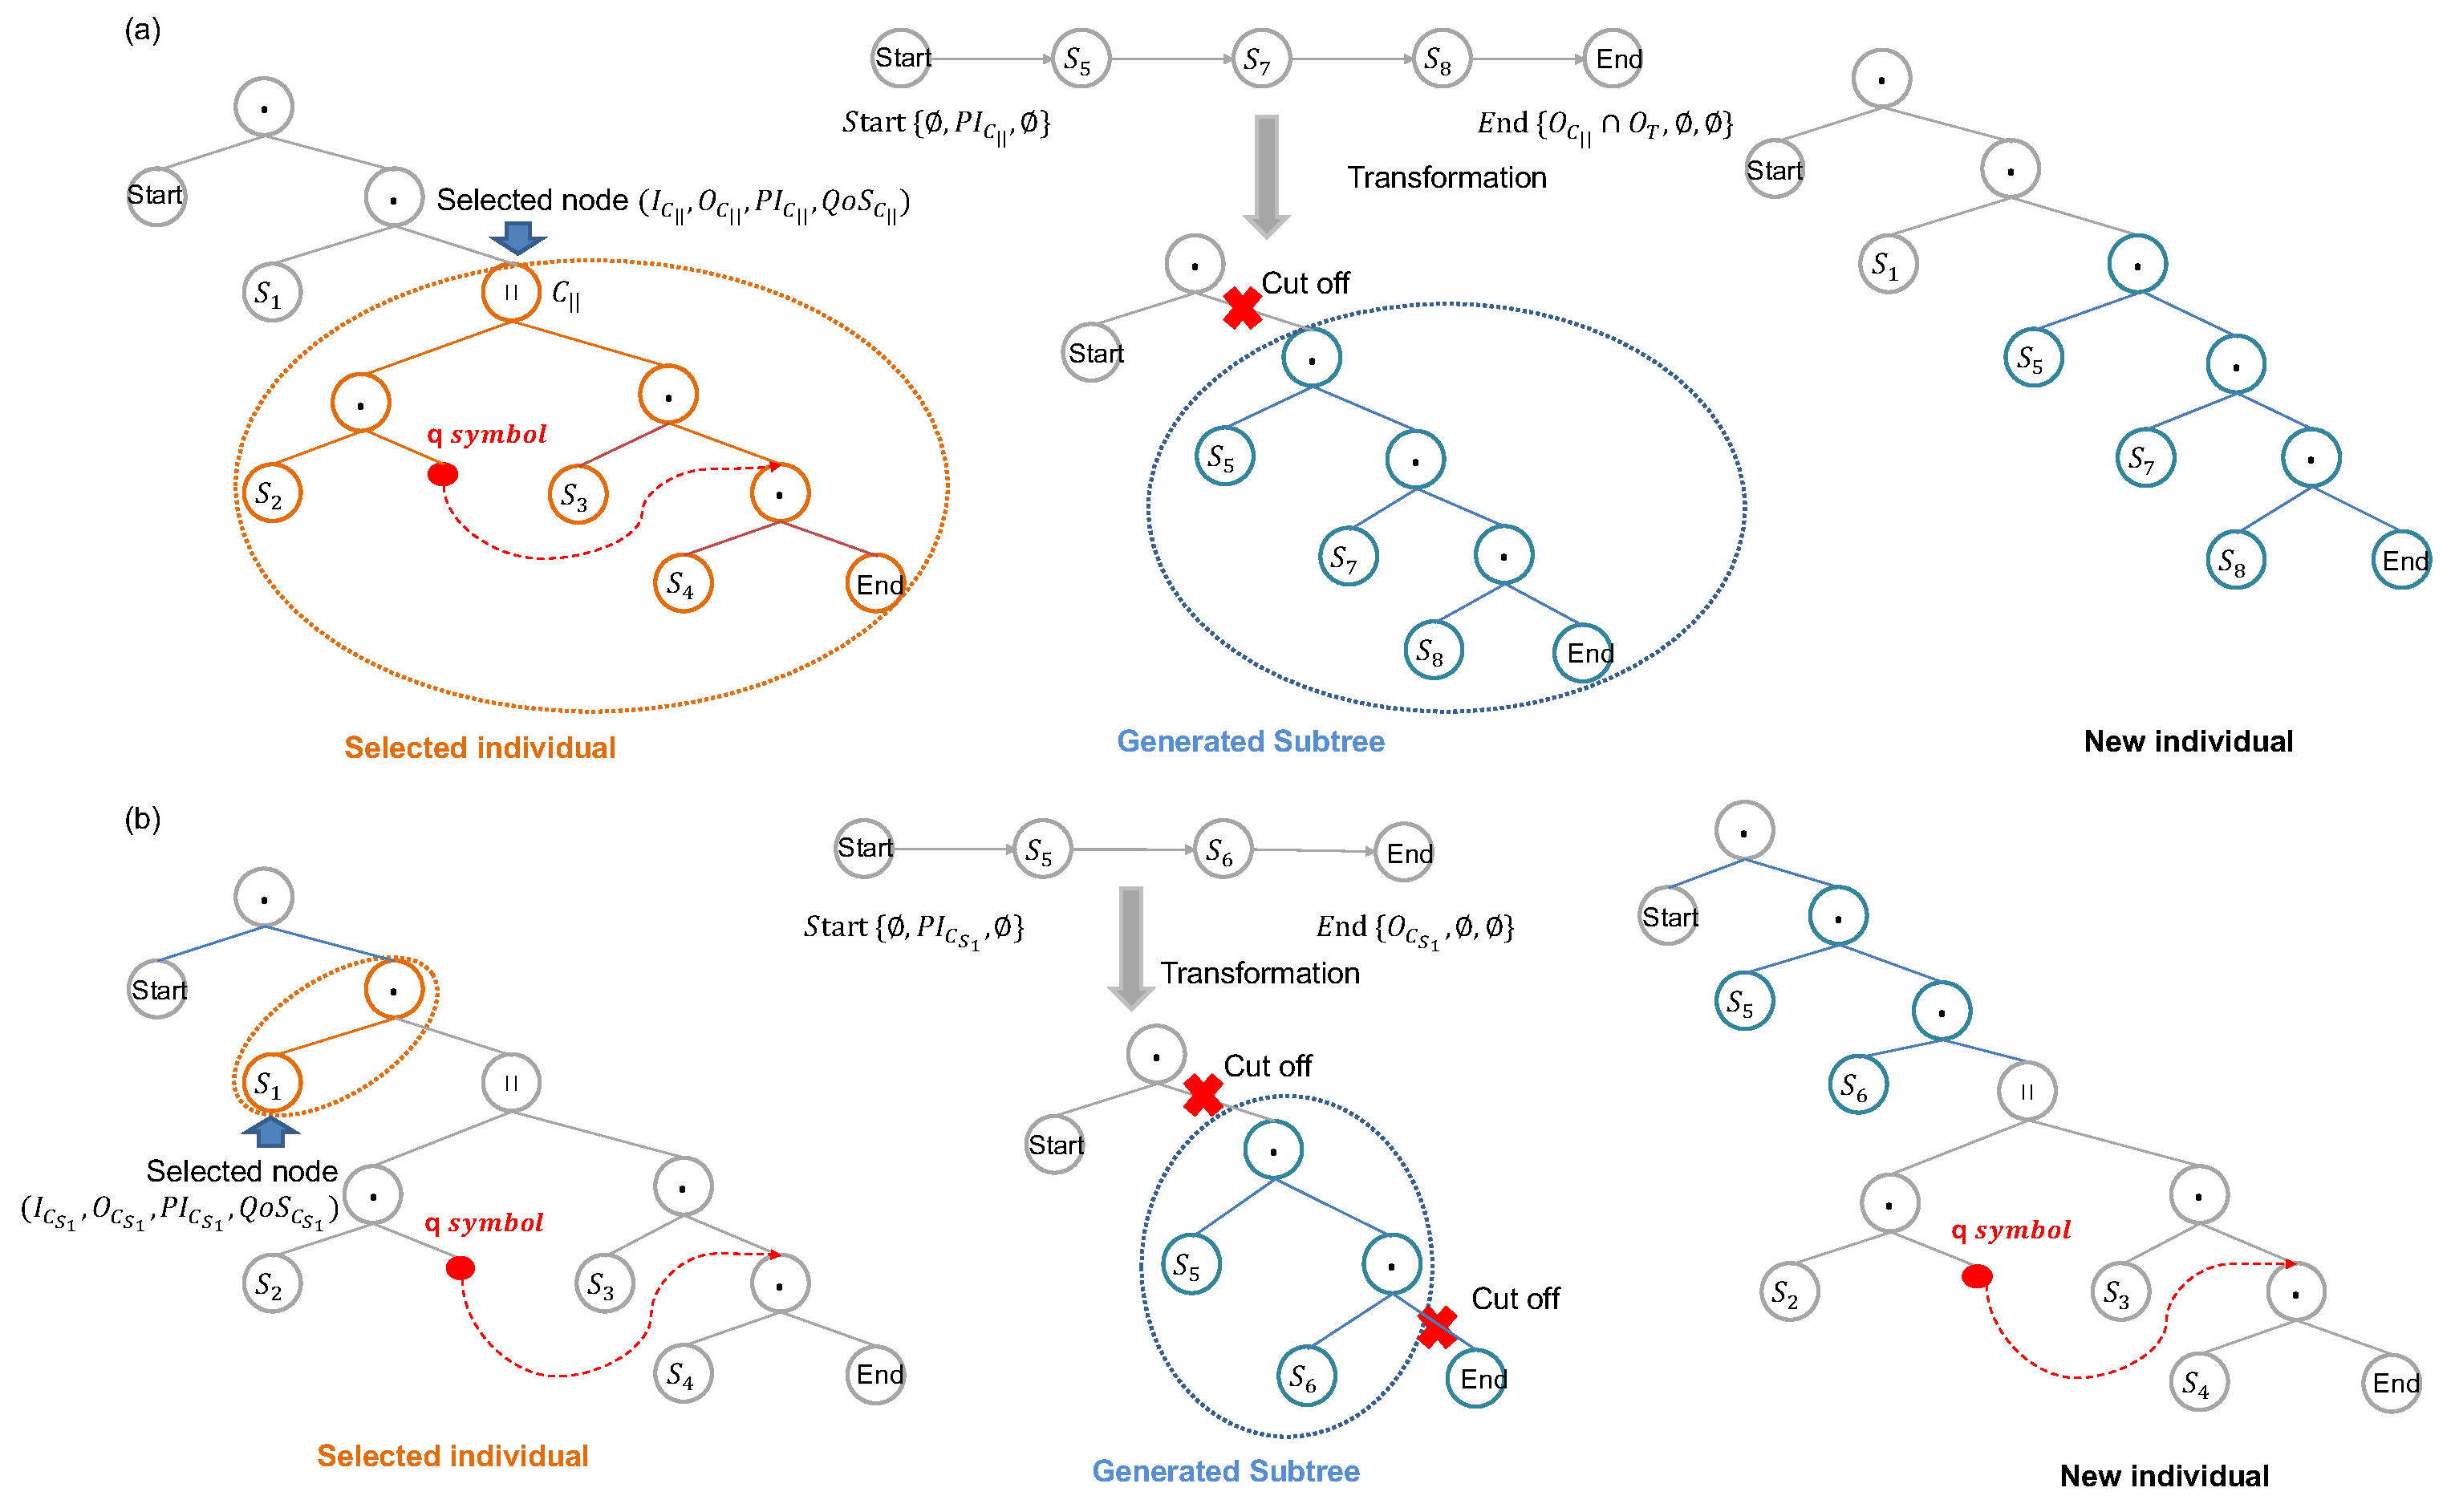
\includegraphics[scale=.23]{mutationExample.pdf}}
\fbox{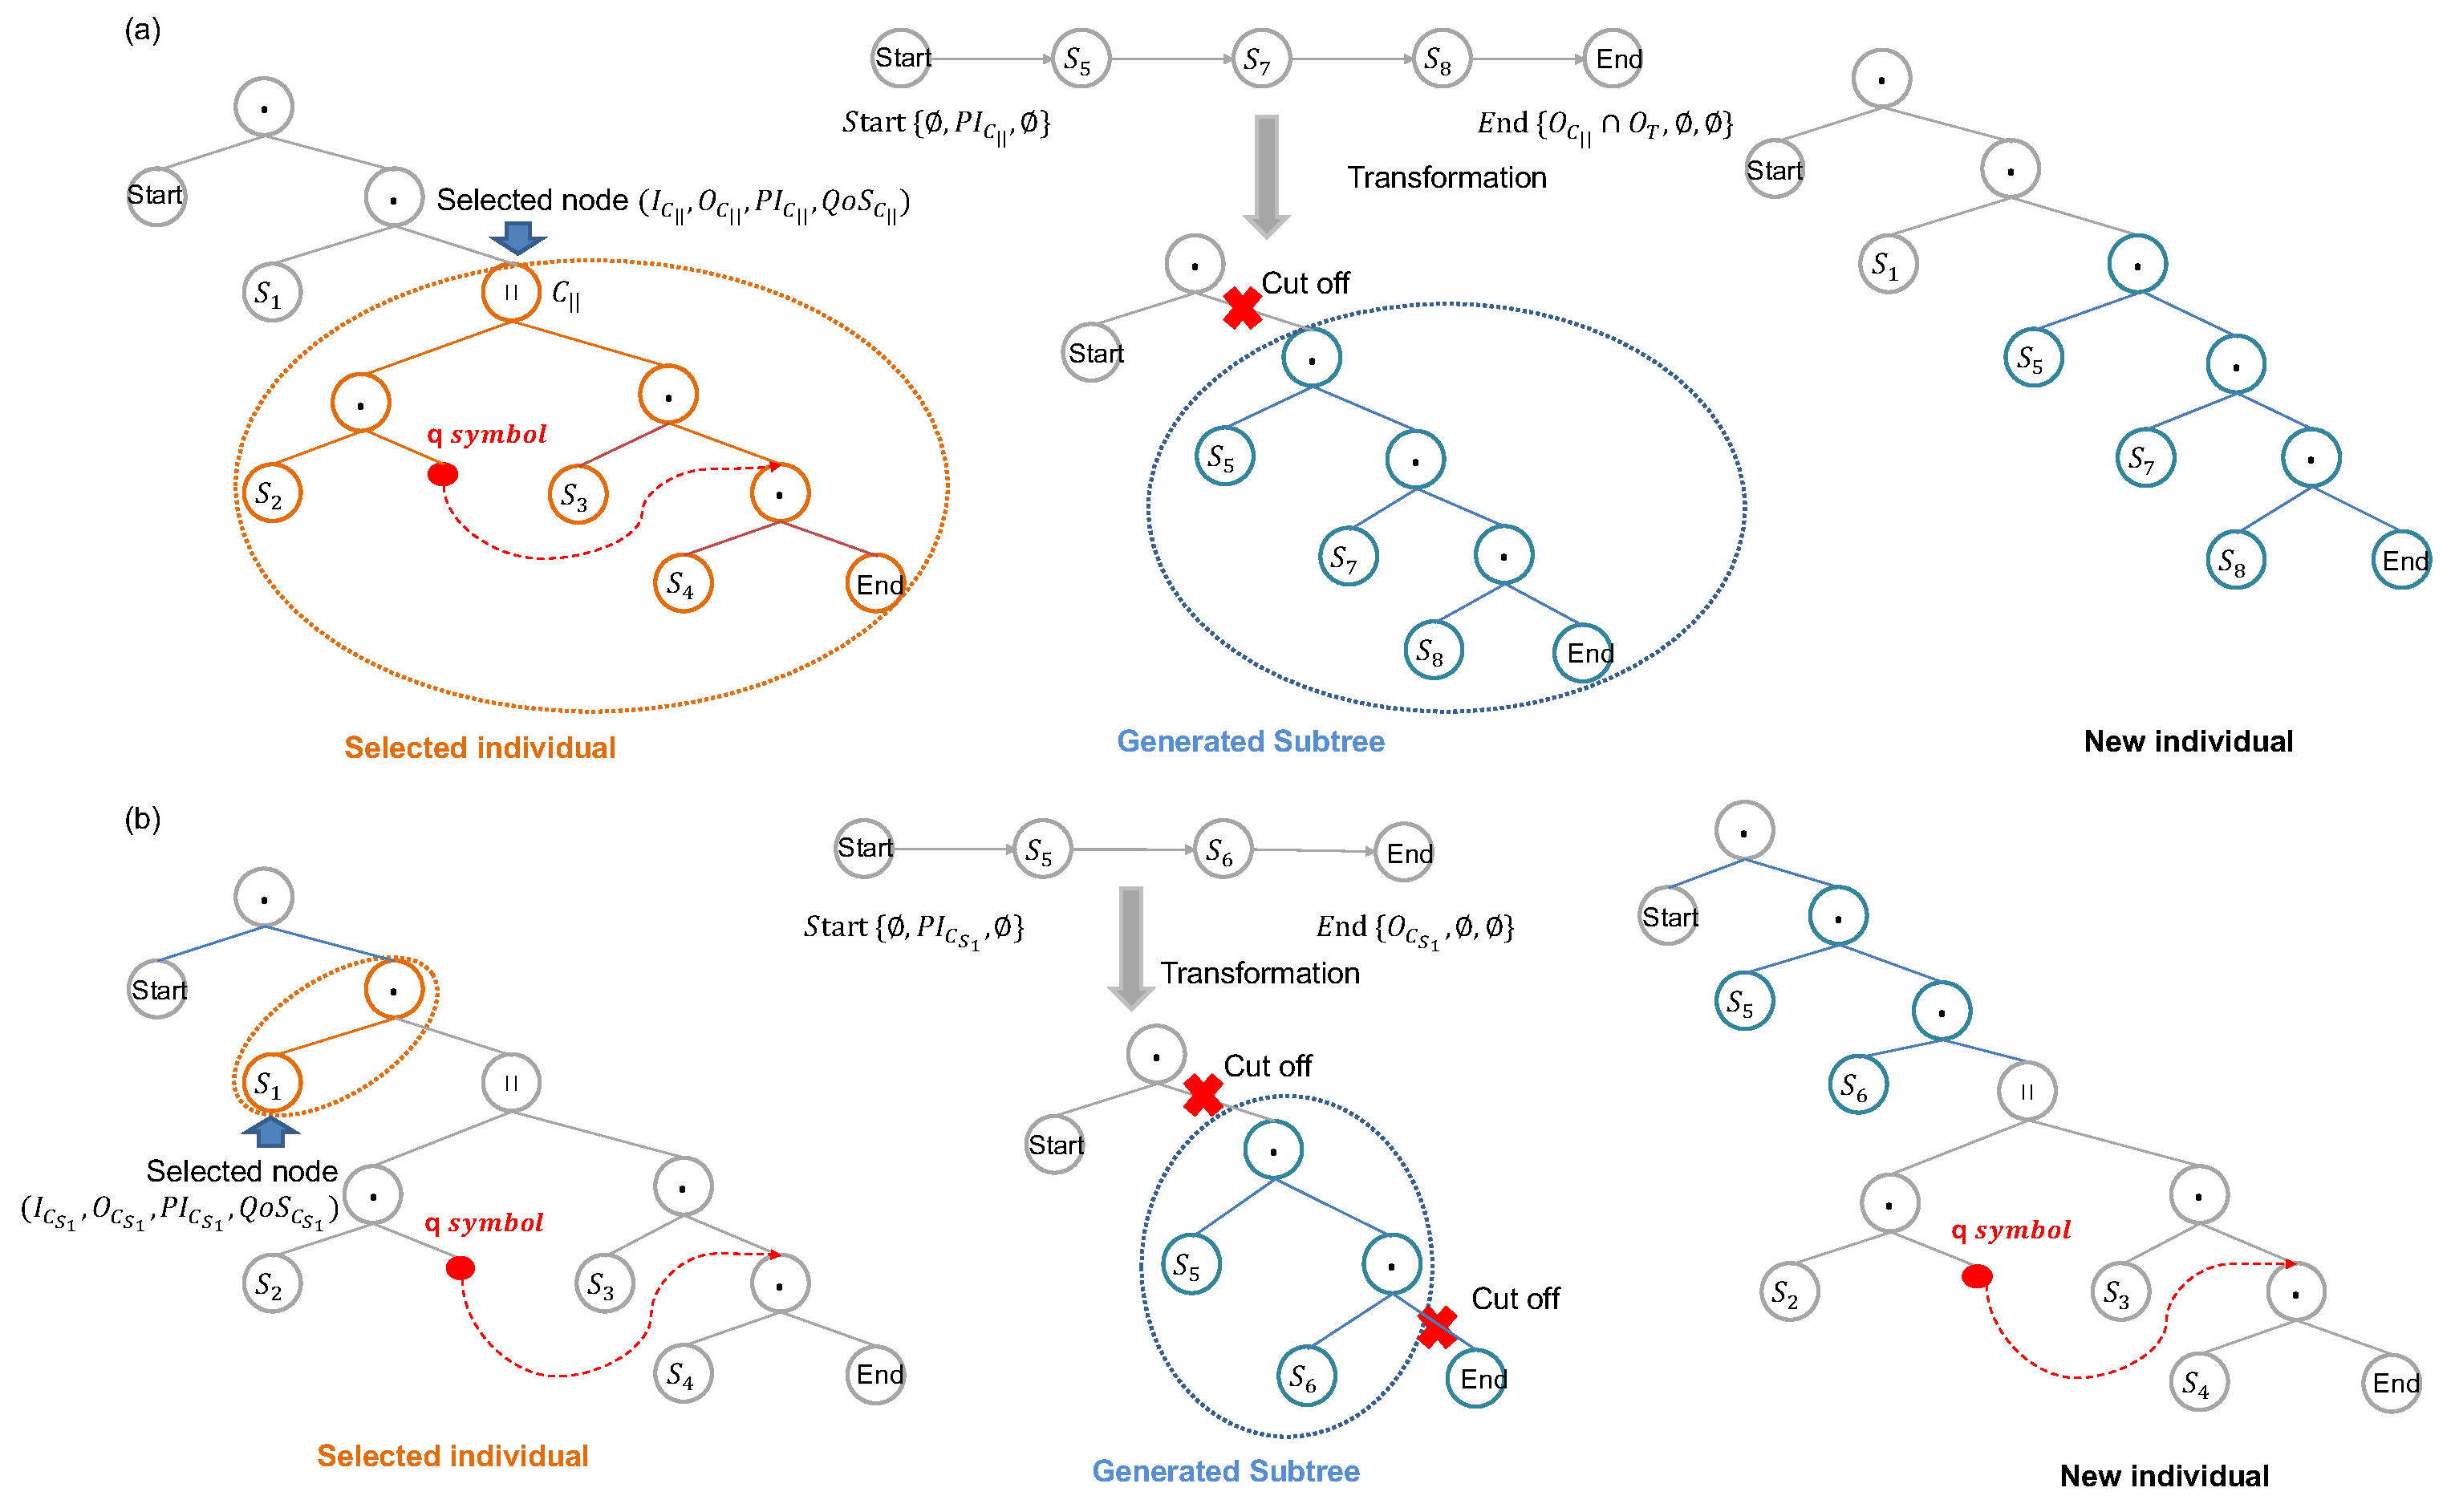
\includegraphics[width=\textwidth]{mutationExample.pdf}}
 \caption{Examples of two mutations on terminal and functional nodes}
 \label{mutationExample}
\end{figure}

Note: The set of available nodes considered for crossover  and mutation do not include $Start$ and $End$, and their parent nodes, because these nodes remain the same for all individuals.  In addition, the nodes selected for crossover and mutation must not break the functionality of $q$ symbols. For example, in Fig. \ref{fig:ExampleOfRepresentation}, both sequential composition $\cse_2$ and $\cse_3 $ are not considered for crossover and mutation as they break the edge of $q$ symbol, but the parallel composition $\cse_{\parallel}$ can be considered for genetic operations, as it may bring a new fully functional $q$ symbol or a subtree without $q$ symbol involved. The pointed subtree $\cse_4$ could also be selected for genetic operations. 
%=================================================================================================== Experiments
\section{Experiment Study for GP-based Approach}\label{experiment_study}

We have conducted experiments to evaluate our proposed approach. 
For our experiments we have used the benchmark datasets originating from OWLS-TC \cite{kuster2008opossum} , which have been extended with real-world QoS attributes and five composition tasks \cite{ma2015hybrid}. To explore the effectiveness and efficiency of our proposed GP-based approach, we compare it against one recent GP-based approach \cite{ma2015hybrid}. For that we have extended the later approach by our proposed comprehensive quality model, so that semantic matchmaking quality can be computed based on the parent-child relationship in the underlying tree representations. 

%Describe the computer environment that you have used for your experiments!

To assure a fair comparison we have used exactly the same parameter settings as in \cite{ma2015hybrid}. In particular, the GP population size has been set to 200, the number of generations to 30, the reproduction rate to 0.1, the crossover rate to 0.8, and the mutation rate to 0.1. We have run every experiment with 30 independent repetitions. Without considering any users' true service composition preferences, the weights in fitness function in Eq. (\ref{eq_fitness}) have been are configured simply to balance semantic matchmaking quality and QoS. Particularly, $w_{1}$ and $w_{2}$ are both set to 0.25, while $w_{3}$, $w_{4}$, $w_{5}$, and $w_{6}$ are all set to 0.125. The parameter $p$ of $type_{link}$ is set to 0.75 ($plugin$ match) in accordance with the recommendation in \cite{lecue2009optimizing}. 

%Why is it fair to use the same parameter settings as in \cite{ma2015hybrid}? Wouldn't it be fair to choose parameter settings that we like and then run experiments with both approaches using the same parameter settings?

Our experiments indicate that our method can work consistently well under valid weight settings and parameter $p$ to be decided by users' preferences in practice.

%========================================================================================= Comparison
\subsection{Comparison against a previous GP-based approach}\label{comparisonTest2}

Table~\ref{meanFitness_GP} shows the fitness values obtained by the two GP-based approaches. To compare the results, an independent-samples T-test over 30 runs has been conducted. The results show that our GP-based approach outperforms the previous GP-based approach \cite{ma2015hybrid} in finding more optimized composition solutions for Tasks 3 and 4. (Note: the P-values are lower than 0.0001). For Tasks 1, 2 and 5, both approaches achieve the same fitness. Therefore, the overall effectiveness of our proposed approach is considered to be better. 

%Why have we conducted a independent-samples T-test rather than a Wilcoxon test?
%We should explain better what we want to emphasize by saying "note: the P-values are lower than 0.0001"
\begin{table}[h!tb]
\footnotesize
\centering
\caption{Mean fitness values for our approach in comparison to \cite{ma2015hybrid}\\ (Note: the higher the fitness the better)}
\label{meanFitness_GP}
\begin{tabular}{l|l|l}
\hline
\multicolumn{1}{c|}{Task} & Our GP-based approach                  & Ma et al. approach \cite{ma2015hybrid}  \\ \hline
OWL-S TC1                     & 0.923793 $\pm$ 0.000000                & 0.923793 $\pm$ 0.000000                   \\ \hline
OWL-S TC2                     & 0.933026 $\pm$ 0.000000                & 0.933026 $\pm$ 0.000000                   \\ \hline
OWL-S TC3                     & 0.870251 $\pm$ 0.000000 $\uparrow$     & 0.832306 $\pm$ 0.008241                   \\ \hline
OWL-S TC4                     & 0.798137 $\pm$ 0.007412 $\uparrow$     & 0.760146 $\pm$ 0.005044                   \\ \hline
OWL-S TC5                     & 0.832998 $\pm$ 0.000000                & 0.832998 $\pm$ 0.000000                   \\ \hline
\end{tabular}
\end{table}

Table~\ref{meanTime} shows the execution times observed for the two GP-based approaches. Again an independent-samples T-test over 30 runs has been conducted. For Tasks 1 and 2 both approaches need about the same time, while for Tasks 3,4, and 5 our approach needs slightly more time. (Note: the P-values are lower than 0.0001). However, even in the worst case it exceeds \cite{ma2015hybrid} by no more than 1 second, which is acceptable for most real-word scenarios. Hence, in terms of efficiency our approach is comparable to \cite{ma2015hybrid}.
\begin{table}[h!tb]
\footnotesize
\centering
\caption{Mean execution time (in ms) for our approach in comparison to \cite{ma2015hybrid}\\ (Note: the shorter the time the better)}
\label{meanTime}
\begin{tabular}{l|l|l}
\hline
\multicolumn{1}{c|}{Task} & Our GP-based approach            & Ma et al. approach \cite{ma2015hybrid}     \\ \hline
OWL-S TC1                     & 7396.366667 $\pm$  772.408168    &  7310.866667  $\pm$952.701775                       \\ \hline
OWL-S TC2                     & 2956.133333  $\pm$ 761.350965    &  3036.966667 $\pm$ 777.121101                       \\ \hline
OWL-S TC3                     & 1057.266667  $\pm$ 174.405183    &  763.800000 $\pm$ 221.241232  $\downarrow$          \\ \hline
OWL-S TC4                     & 4479.466667  $\pm$ 519.767172    &  3068.800000 $\pm$ 472.013106  $\downarrow$        \\ \hline
OWL-S TC5                     & 6276.533333  $\pm$ 1075.102328   &  5030.200000 $\pm$ 991.863812 $\downarrow$         \\ \hline
\end{tabular}
\end{table}

The experiments confirm that there is a trade-off between fitness and execution time in GP-based service composition. It can be argued that our proposed approach achieves a better balance as the computed solutions observe a significantly higher fitness while there is a moderate increase in execution time compared to \cite{ma2015hybrid}. 

%========================================================================================= Discussion
\subsection{Further Discussion}
For Tasks 3 and 4, the optimized composition solutions obtained by the two approaches are shown in Fig.~\ref{example1and2}(a) and Fig.~\ref{example1and2}(b), respectively. The functional and nonfunctional descriptions of all services involved in these solutions are listed in Fig.~\ref{example1and2}(c). 

%For Datasets 3 and 5, the optimized composition solutions obtained by the two approaches are shown in Fig.~\ref{example1and2}(a) and Fig.~\ref{example1and2}(b), respectively. The functional descriptions of all services involved in these solutions are listed in Fig.~\ref{example1and2}(c). For Dataset 5 the composition task is $T=( \{ duration, city, country \}, \{ weatherseason, map, hotel\})$. The optimized composition solutions obtained by the two approaches are identical, even though different representations have been used during GP.  

%change "Task" to "Dataset" in the figure,
% there is only one dataset with 5 different tasks
%Should we move the composition task into the figure so that readers don't need to look for it in the text?

\begin{figure}[h!tb]
\centering
%\fbox{\includegraphics[scale=.30]{example1and2.pdf}}
\fbox{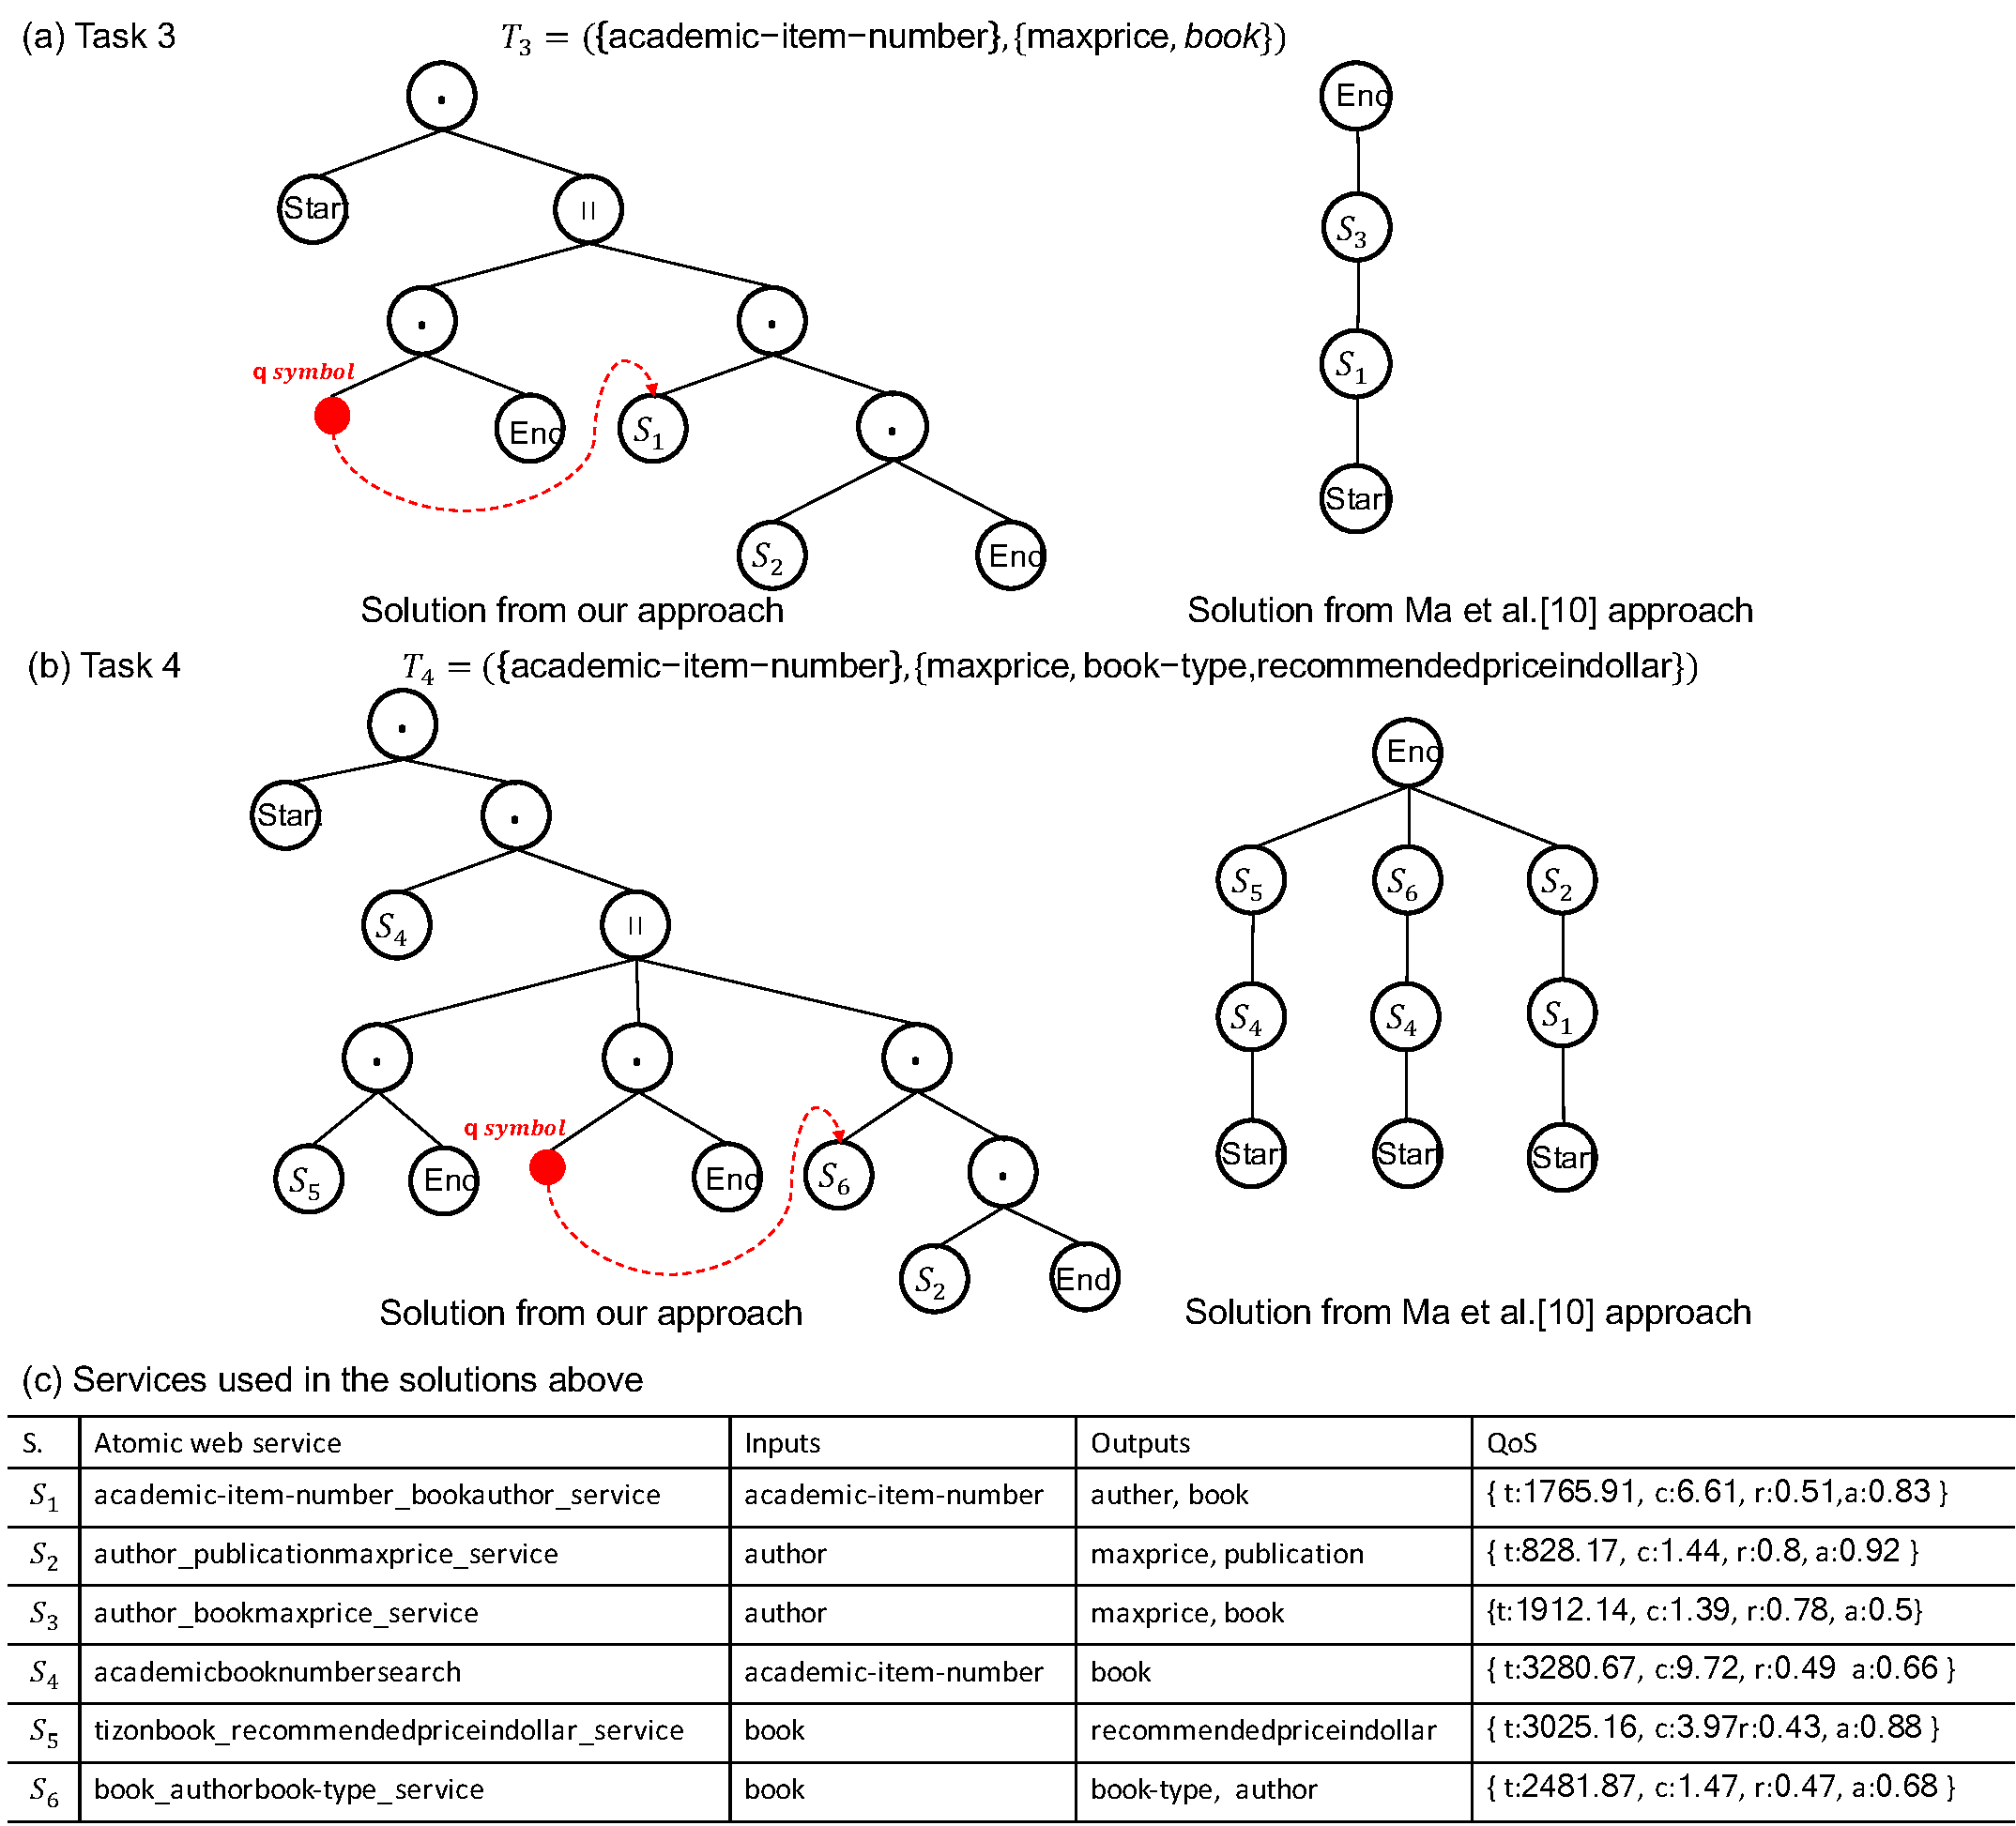
\includegraphics[width=.9\textwidth]{experimentExample(p-symbol).pdf}}
 \caption{Example of best solutions using the two GP-based approaches}
 \label{example1and2}
\end{figure}
\noindent For Task 3 the composition task is $T_3=(\{academic$-$item$-$number\},\{ book, maxprice\})$. The best composition solutions obtained by the two approaches are different, see Fig.~\ref{example1and2}. Both solutions have the same semantic matchmaking quality as the matchmaking type of all links is $exact$ match. However, both solutions differ in their QoS. This is due to the different services that are involved: $S_2$ versus $S_3$. The QoS of $S_2$ is much better that of $S_3$. Consequently, the best composition solution obtained by our approach has higher fitness according to our quality model.  It is interesting to observe that the best composition solution obtained by our approach for Task 3 can be evolved from the best composition solution in  \cite{ma2015hybrid} just by a single mutation on $S_3$ using available inputs.


For Task 4 the composition task is $T_4=(\{academic$-$item$-$number\},\{ maxprice, book-type,recommendedpriceindollar\})$. The best solutions obtained by the two approaches are also different, see Fig.~\ref{example1and2}. Note that solution generated by our approach is composed of four atomic services ($S_4$, $S_5$, $S_6$ and $S_2$) while the solution generated by approach \cite{ma2015hybrid} is composed of  five atomic services ($S_4$, $S_5$, $S_6$, $S_1$ and $S_2$). Both solutions have the same semantic matchmaking quality as the matchmaking type of all links is $exact$ match. However, the overall QoS of our approach is better. This is due to the additional $S_1$ in their approach, which has a significant negative impact on QoS.

We observe from above examples that our approach is able to produce better solutions because our proposed representation keeps available inputs and least required outputs of each node on the tree which unlocks more opportunities for 
mutation and crossover rather than restricting them to the previously used inputs and outputs only.

%\begin{figure}[h!tb]
%\centering
%\fbox{\includegraphics[scale=.30]{example1and2.pdf}}
%\fbox{\includegraphics[width=.9\textwidth]{example1and2.pdf}}
% \caption{Example of best solutions using the two GP-based approaches}
% \label{example1and2}
%\end{figure}

%It may due to the structure of the introduced representation that brings more possibilities of different combined functionality via functional nodes and more flexible mutation operator that utilises available inputs to generate more varieties of subtrees.

%How about the best solutions obtained with both approaches for Dataset 4? Can we look at them?
%=================================================================================================== Conclusion
\section{Summary for our GP-based Approach}\label{summary2}

In this work, we introduces a novel GP-based approach to comprehensive quality-aware semantic Web service composition. In particular, a tree-like representation is proposed to direct cope with the evaluation of semantic matchmaking quality. Meanwhile, crossover and mutation methods are proposed to maintain the correctness of individuals. The experiment  shows that our proposed approach could effectively produce better solutions in both semantic matchmaking quality and QoS than the existing approach.

\section{Conclusion}\label{summary2}
In the preliminary work, we propose and formalize a novel and effective comprehensive quality model for simultaneously optimize QoS and quality of semantic matchmaking. Apart from that, two novel and effective EC-based methods are proposed for comprehensive quality-aware semantic Web service composition. In particular, indirect and direct representations are designed for studying their effectiveness and efficiency along with newly developed evolutionary operators. Overall experimental studies show both two methods reach good performances comparing to existing works. We also find that our PSO-based approach utilizing an indirect representation outperforms our GP-based approach utilizing a direct representation for finding more effective solutions. These findings motivate us to work on a more effective indirect presentation along with PSO-based memetic method.
%=================================================================================================== Bibliography
%The bibliography can be improved. Remove unnecessary bibliographic information from some of the items. Make sure that QoS is not shown as qos.

%\chapter{Proposed Contributions and Project Plan}\label{C:plan}

\section{Proposed Contributions}

In the previous chapter, some preliminary work has been done to the investigation the performances of direct representation and indirect representation on the proposed PSO-based approach and GP-based approach respectively. We have shown that those two approaches outperform some recent existing EC-based approaches using our proposed comprehensive quality model for evaluation. In addition to carrying a further research on the first objective, the rest three objectives outlined in the proposal will be investigated. This chapter presents the proposed contribution and project plan to guide the research direction for the thesis.

\begin{enumerate}
 \item This thesis will develop a new fully automated semantic web service composition approach for simultaneously optimising the quality of semantic matchmaking and QoS. This is expected to be more effective and efficient at handling combinatorial optimisation problem in service composition, which is done by relying on a most effective representation, a comprehensive quality model and a motivated EC-based method with local search or AI planning techniques.

\item This thesis will extend on previous many-objective web service composition approach to effective and efficient explore the Pareto front of comprehensive quality-aware service composition. Apart from that, conditional constraints in SLA and customised matchmaking level is expected to handle conditional constraints on each independent objectives in comprehensive quality mode. Simutenaneouly taking all these necessary requirements is not considered in any past research. 

\item This thesis will develop an effective and efficient EC-based hybrid approach for dynamic web service composition problem. This approach is expected to better handle composition environment changes. In particular, the changes of QoS, Ontology and service repository (i.e., service failure and new service registration). These changes are not fully studied in the past and solved using the EC-based approach in the research area.

\item This thesis will develop EC-based hybrid approaches to a more complex and realistic semantic web service composition based on not only inputs and outputs, but precondition and postcondition. This is expected to develop a general mechanism for supporting all the service composition constructs. Those occasionally considered precondition and postconditions are not fully studied for supporting all the composition constructs and not employed in a fully automated approach either.
\end{enumerate}

\section{Overview of Project Plan}

Six milestones for PhD project are defined in the initial research plan shown in Table \ref{tab:projectOverview}. The first phase of this plan has been completed, which comprising of literature view, an initial work on comprehensive quality-aware semantic web service composition and a research proposal writing.  The second phase is related to the first objective of this proposal and is currently in progress, which is covered in Chapter \ref{C:preliminary} of the proposal. The remaining phases are expected to be completed as planned.

\begin{table}
\small
\centering
\caption{The milestones of PhD project plan.}
\vspace{0.2cm}
\begin{tabular}{|c|p{100mm}|l|}
\hline
Phase & Description & Duration (months) \\ \hline
1 & Reviewing literature, developing initial EC-based composition approach, and writing the proposal & 9 (Complete)  \\
2 & Develop Hybrid approaches to comprehensive quality-aware automated web service composition & 6 (In progress) \\
3 & Develop multi-objective approaches to optimise the comprehensive quality for fully automated service composition & 7 \\
4 & Develop hybrid techniques to support dynamic semantic web service composition effectively & 8 \\
5 & Develop hybrid approaches for semantic web service compositions based on preconditions and effects & 3 \\
6 & Writing the thesis & 6 \\ \hline
\end{tabular}
\label{tab:projectOverview}
\end{table}

\section{Project Timeline}

Table \ref{tab:projectTimeline} provide an estimated timeline comprising of the minor goals and milestones, which is expected to serve as a guide and be completed through the PhD project.

\begin{table}
\small
\centering
\caption{Project timeline for the remaining 24 months.}
\vspace{0.2cm}
\begin{tabular}{|c|p{50mm}||ccc|ccc|ccc|ccc|}
\hline
& & \multicolumn{12}{c|}{Time in Months} \\ \hline
Phase & Task                                                & 2 & 4 & 6  & 8 & 10 & 12  & 14 & 16 & 18  & 20 & 22 & 24 \\ \hline
n/a & Updating the literature review
                                                            & x & x & x & x & x & x & x & x & x & x & x & x \\ 
2 & Developing indirect representation utilise in a hyper-heuristics methods
                                                            & x & x &    &   &   &    &   &   &    &   &   &   \\
3 & Investigating unconstrained MO optimisation for semantic quality-aware service composition
                                                            &   & x & x  &   &   &    &   &   &    &   &   &   \\
3 & Improving performance of MO approach by integrating other techniques  
                                                            &   &   &  x & x &   &    &   &   &    &   &   &   \\
3 & Extending MO approach to handle constraints on SLA and semantic matchmaking level
                                                            &   &   &    &   & x & x   &   &   &    &   &   &   \\
4 & Develop EC-based hybrid approach to handle changes in QoS and Ontology
                                                            &   &   &    &   &   & x  & x &   &    &   &   &   \\
4 & Develop EC-based hybrid approach to handle service failure and new service registration
                                                            &   &   &    &   &   &    & x & x &    &   &   &   \\
5 & Develop EC-based hybrid approach to handle preconditions and effects.
                                                            &   &   &    &   &   &    &   & x & x  &   &   &   \\
6 & Writing the first thesis draft  
                                                            &   &   &    &   &   &    &   &   &    & x & x &   \\
6 & Editing the final draft
                                                            &   &   &    &   &   &    &   &   &    &   & x & x \\
\hline
\end{tabular}
\label{tab:projectTimeline}
\end{table}

\section{Thesis Outline}

The following is an outline of the PhD thesis,  in which Chapter 6 may be replaced by Chapter 7 since it is an optimal objective.

\begin{itemize}
 \item \textit{Chapter 1: Introduction}\\
 This chapter will introduce the thesis, providing a problem statement and motivations, defining research goals and contributions, and outlining the structure of this dissertation.
 \item \textit{Chapter 2: Literature Review}\\
 The literature review will examine the existing work on Web service composition, discussing the fundamental concepts in this field in order to provide the reader with the necessary background. Multiple sections will then follow, each of them analysing the problem from a different angle, considering issues such as QoS-aware composition, semantic selection, and composition methods for dynamic environments. The focus of this review is on investigating composition techniques that are based on Evolutionary Computation and on AI planning.
 \item \textit{Chapter 3: A Hybrid Planning/EC Approach to Web Service Composition}\\
 This chapter will introduce a new approach to Web service composition that combines elements of AI planning with Evolutionary Computation techniques. One of the critical aspects of this new approach is the representation of composition candidates, therefore multiple representation possibilities will be analysed and compared to identify the most suitable model. 
 \item \textit{Chapter 4: Many-Objective Optimisation of Compositions with Multiple Paths}\\
 In this chapter, many-objective optimisation techniques will be employed to allow each quality dimension of compositions to be improved independently. After investigating these techniques in an unconstrained manner, SLA constraints will also be considered. While these constraints add to the complexity of the problem, they may also prove useful when filtering potential solutions, thus experiments comparing the constrained and unconstrained approaches will be conducted.
 \item \textit{Chapter 5: Semantic Web Service Selection in a Planning-Based Composition Technique}\\
 A novel semantic approach for selecting which services are to be included in the composition will be proposed in this chapter. This approach focuses on selecting candidate services to be used in a planning-based composition technique without relying on precalculated semantic distances, as existing approaches have done. A comparison will be performed between this novel approach and the those that rely on precalculations.
 \item \textit{Chapter 6: EC-Based Compositions in a Dynamic Environment}\\
 This chapter will extend the composition technique discussed throughout this thesis to work in dynamic environments. Firstly, a way of re-optimising solutions as quality values fluctuate will be proposed, and then an approach for responding to service faults will be discussed. The extended technique will be compared against the existing dynamic composition approaches, which do not use EC techniques, to establish whether there are quality gains in the solutions produced.
 \item \textit{Chapter 7: Conclusions and Future Work}\\
 In this chapter, conclusions will be drawn from the analysis and experiments conducted in the different phases of this research, and the main findings for each one of them will be summarised. Additionally, future research directions will be discussed.
\end{itemize}


\section{Resources Required}

\subsection{Computing Resources}
An experimental approach will be adopted in this research, entailing the execution of experiments that are likely to be computationally expensive. The ECS Grid computing facilities can be used to complete these experiments within reasonable time frames, thus meeting this requirement.

\subsection{Library Resources}
The majority of the material relevant to this research can be found online, using the university's electronic resources. Other works may either be acquired at the university's library, or by soliciting assistance from the Subject Librarian for the fields of engineering and computer science.

\subsection{Conference Travel Grants}
Publications to relevant venues in this field are expected throughout this project, therefore travel grants from the university are required for key conferences.


%%%%%%%%%%%%%%%%%%%%%%%%%%%%%%%%%%%%%%%%%%%%%%%%%%%%%%%

\backmatter

%%%%%%%%%%%%%%%%%%%%%%%%%%%%%%%%%%%%%%%%%%%%%%%%%%%%%%%


%\bibliographystyle{ieeetr}
\bibliographystyle{acm}
\bibliography{bibliography}


\end{document}
